%!TEX program = xelatex
\documentclass[a4paper,12pt]{article}
\usepackage{fontspec}
\setmainfont{Times New Roman}
\setsansfont{Arial}
\setmonofont[Scale=0.85]{Consolas}
\usepackage{xurl}
\emergencystretch=3em
\tolerance=1500
\hbadness=1500

\usepackage{geometry}
\geometry{
    left=2.5cm,
    right=2cm,
    top=2.5cm,
    bottom=2.5cm
}

\usepackage{graphicx}
\usepackage{float}
\usepackage{longtable}
\usepackage{booktabs}
\usepackage{array}
\usepackage{tabularx}
\usepackage{multirow}
\usepackage{multicol}
\usepackage{caption}
\usepackage{subcaption}
\usepackage{setspace}
\usepackage{indentfirst}
\usepackage{amsmath, amssymb, amsfonts}
\usepackage{lastpage}
\usepackage{fancyhdr}
\usepackage{xcolor}
\usepackage{tcolorbox}
\usepackage{listings}
\usepackage{tikz}
\usepackage{pdflscape}
\usepackage{hyperref}

\hypersetup{
    urlcolor=blue,
    linkcolor=black,
    citecolor=black,
    colorlinks=true,
    pdftitle={Báo cáo đồ án chuyên ngành - Phát triển game Convergence Chess},
    pdfauthor={Nhóm thực hiện Convergence Chess}
}

% Việt hóa các nhãn mặc định theo chuẩn Sentence case
\renewcommand{\contentsname}{Mục lục}
\renewcommand{\listfigurename}{Danh mục hình ảnh}
\renewcommand{\listtablename}{Danh mục bảng biểu}
\renewcommand{\figurename}{Hình}
\renewcommand{\tablename}{Bảng}
\renewcommand{\refname}{Tài liệu tham khảo}

% Khung hộp ghi chú và khung chừa chỗ ảnh chụp màn hình in-game
\newtcolorbox{notebox}[1]{
    colback=blue!4!white,
    colframe=blue!55!black,
    fonttitle=\bfseries,
    title=#1,
    boxrule=0.6pt,
    arc=3pt
}

\newcommand{\screenshotplaceholder}[2]{%
    \begin{tcolorbox}[
        colback=gray!8!white,
        colframe=gray!60!black,
        boxrule=0.8pt,
        arc=3pt,
        width=0.92\textwidth,
        halign=center,
        top=1.2cm,
        bottom=1.2cm
    ]
        \textbf{[Khung chờ ảnh chụp màn hình thực tế trong Unity]} \\[0.3cm]
        \texttt{#1} \\[0.25cm]
        \small \textit{Hướng dẫn chụp bổ sung: #2}
    \end{tcolorbox}
}

% Style mã nguồn C# và Python
\definecolor{codebg}{rgb}{0.96, 0.98, 0.96}
\definecolor{keywordcolor}{rgb}{0.45, 0.0, 0.65}
\definecolor{stringcolor}{rgb}{0.0, 0.45, 0.0}
\definecolor{commentcolor}{rgb}{0.25, 0.45, 0.45}
\definecolor{frameborder}{rgb}{0.3, 0.3, 0.3}

\lstdefinelanguage{CSharp}{
    language=[Sharp]C,
    morekeywords={async,await,var,dynamic,yield,get,set,readonly,ushort,ulong,record,init}
}

\lstdefinestyle{csharpstyle}{
    language=CSharp,
    backgroundcolor=\color{codebg},
    basicstyle=\ttfamily\footnotesize,
    keywordstyle=\color{keywordcolor}\bfseries,
    stringstyle=\color{stringcolor},
    commentstyle=\color{commentcolor}\itshape,
    frame=single,
    rulecolor=\color{frameborder},
    framerule=0.5pt,
    framesep=6pt,
    tabsize=4,
    showspaces=false,
    showstringspaces=false,
    breaklines=true
}

\newcolumntype{C}[1]{>{\centering\arraybackslash}p{#1}}
\newcolumntype{L}[1]{>{\raggedright\arraybackslash}p{#1}}
\newcolumntype{Y}{>{\raggedright\arraybackslash}X}

% Cấu hình Header & Footer
\setlength{\headheight}{42pt}
\pagestyle{fancy}
\fancyhead{}
\fancyhead[L]{
    \begin{tabular}{rl}
        \begin{picture}(25,15)(0,0)
            \put(-5,-15){
\includegraphics[width=16mm, height=11.5mm]{hcmut.png}}
        \end{picture} &
        \begin{tabular}{l}
            \textbf{\small Trường Đại học Bách khoa Tp. Hồ Chí Minh} \\
            \textbf{\small Khoa Khoa học và Kỹ thuật Máy tính}
        \end{tabular}
    \end{tabular}
}
\fancyhead[R]{\small \textit{Convergence Chess}}
\fancyfoot{}
\fancyfoot[L]{\scriptsize \ttfamily Đồ án chuyên ngành - CO4029 - HK261}
\fancyfoot[R]{\scriptsize \ttfamily Trang {\thepage}/\pageref{LastPage}}
\renewcommand{\headrulewidth}{0.4pt}
\renewcommand{\footrulewidth}{0.4pt}

% Cấu hình chiều sâu mục lục và đánh số mục
\setcounter{secnumdepth}{4}
\setcounter{tocdepth}{3}
\makeatletter
\newcounter{subsubsubsection}[subsubsection]
\renewcommand\thesubsubsubsection{\thesubsubsection.\@alph\c@subsubsubsection}
\newcommand\subsubsubsection{\@startsection{subsubsubsection}{4}{\z@}%
    {-3.0ex\@plus -1ex \@minus -.2ex}%
    {1.2ex \@plus .2ex}%
    {\normalfont\normalsize\bfseries}}
\newcommand*\l@subsubsubsection{\@dottedtocline{4}{10.0em}{4.1em}}
\newcommand*{\subsubsubsectionmark}[1]{}
\makeatother

\begin{document}
\onehalfspacing

% ======================== TRANG BÌA ========================
\begin{titlepage}
\begin{tikzpicture}[remember picture, overlay]
    % Khung ngoài
    \draw[line width=4pt]
      ([xshift=1.8cm,yshift=-1.8cm]current page.north west)
      rectangle
      ([xshift=-1.8cm,yshift=1.8cm]current page.south east);
    % Khung trong
    \draw[line width=1.5pt]
      ([xshift=2.05cm,yshift=-2.05cm]current page.north west)
      rectangle
      ([xshift=-2.05cm,yshift=2.05cm]current page.south east);
\end{tikzpicture}

\vspace*{-0.8cm}
\begin{center}
    {\large \textbf{ĐẠI HỌC QUỐC GIA THÀNH PHỐ HỒ CHÍ MINH}} \\
    {\large \textbf{TRƯỜNG ĐẠI HỌC BÁCH KHOA}} \\
    {\large \textbf{KHOA KHOA HỌC VÀ KỸ THUẬT MÁY TÍNH}}
\end{center}

\vspace{0.3cm}
\begin{figure}[h!]
    \centering
    
\includegraphics[width=5.2cm]{hcmut.png}
\end{figure}

\vspace{0.1cm}
\begin{center}
    {\LARGE \textbf{BÁO CÁO ĐỒ ÁN CHUYÊN NGÀNH}} \\[0.25cm]
    {\large \textit{(Giai đoạn 1: Khảo sát, thiết kế kiến trúc và thử nghiệm nguyên mẫu)}} \\[0.8cm]

    {\fontsize{21pt}{28pt}\selectfont \textbf{PHÁT TRIỂN GAME}} \\[0.2cm]
    {\fontsize{23pt}{30pt}\selectfont \textbf{CONVERGENCE CHESS}} \\[0.6cm]

    {\large NGÀNH: KHOA HỌC MÁY TÍNH}
\end{center}

\vspace{0.6cm}
\begin{center}
    % Ghi chú: Sinh viên tự cập nhật lại tên Hội đồng, GVHD và Họ tên/MSSV chính xác trước khi nộp
    \begin{tabular}{lll}
        \large \textbf{Hội đồng:} & \large [Cập nhật tên Hội đồng] & \\[0.2cm]
        \large \textbf{GVHD:} & \large [Cập nhật Họ tên GVHD] & \\[0.2cm]
        \large \textbf{SVTH 1:} & \large [Cập nhật Họ tên SV1 - Core, AI, SC] & \large [MSSV 1] \\[0.18cm]
        \large \textbf{SVTH 2:} & \large [Cập nhật Họ tên SV2 - Multiplayer, View] & \large [MSSV 2] \\
    \end{tabular}
\end{center}

\vfill
\begin{center}
    {\large Thành phố Hồ Chí Minh, tháng 12/2026}
\end{center}
\vspace{0.7cm}
\end{titlepage}

% ======================== MỤC LỤC & DANH MỤC ========================
\clearpage
\pagenumbering{roman}
\tableofcontents
\newpage
\listoffigures
\newpage
\listoftables

% ======================== NỘI DUNG CHÍNH ========================
\clearpage
\pagenumbering{arabic}
\setcounter{page}{1}

\section{Giới thiệu đề tài}

\subsection{Bối cảnh và vấn đề đặt ra}
Trong lĩnh vực trò chơi điện tử chiến thuật theo lượt, cờ vua truyền thống từ lâu đã được xem là chuẩn mực kinh điển về chiều sâu tư duy logic và tính cân bằng. Tuy nhiên, đối với nhóm người chơi hiện đại, cờ vua cổ điển tồn tại hai rào cản đáng kể: (i) thời lượng ván đấu kéo dài với nhiều khai cuộc mang tính học thuộc, làm giảm yếu tố bất ngờ; và (ii) cấu trúc luật cố định, thiếu các cơ chế tùy biến đội hình trước trận hoặc nâng cấp sức mạnh quân cờ trong trận như các trò chơi chiến thuật hiện đại.

Ở chiều ngược lại, các biến thể cờ chiến thuật mới nổi thường thiên về yếu tố may rủi hoặc đồ họa bắt mắt mà ít chú trọng đến thiết kế kiến trúc tách biệt giữa luật chơi và phần hiển thị. Điều này gây khó khăn khi vừa cần vận hành mượt mà ở chế độ nhiều người chơi trực tuyến (Online Multiplayer), vừa cần mô phỏng tốc độ cao để huấn luyện Trí tuệ nhân tạo (AI). Bên cạnh đó, nhu cầu cá nhân hóa danh tính người chơi trong không gian 3D (như tạo hình đại diện từ ảnh chân dung thực tế) ngày càng được quan tâm nhưng vẫn còn nhiều thách thức về thời gian xử lý, độ chính xác hình học khuôn mặt 3D và xử lý ánh sáng bề mặt da.

Xuất phát từ các nhận định trên, nhóm thực hiện đề tài \textbf{Phát triển game ``Convergence Chess''} -- một trò chơi cờ chiến thuật 3D trên nền tảng Unity 6 \cite{unity6}, kết hợp cấu trúc di chuyển của cờ vua với cơ chế kinh tế điểm hành động tích lũy (AP), vật cản sinh ngẫu nhiên và đặc biệt là cơ chế \textbf{hợp thể quân cờ} kèm trạng thái đòn bồi (\textbf{Surge}). Dự án đồng thời xây dựng hai hướng tác nhân AI chính là \textbf{Hybrid Bot} (kết hợp tìm kiếm Minimax, học tăng cường PPO \cite{mlagents} và mạng đánh giá nhanh NNUE \cite{nnue}) và \textbf{LLM Bot} (tiến hóa luật đánh giá bằng Mô hình Ngôn ngữ Lớn theo hướng FunSearch \cite{funsearch}), tích hợp chế độ đối kháng trực tuyến qua Photon Fusion 2 \cite{photon_fusion} cùng phân hệ mở rộng tùy biến nhân vật 3D từ ảnh chân dung (Smart Customization).

\subsection{Tổng quan luật chơi và cơ chế cốt lõi của Convergence Chess}
Khác với bàn cờ $8 \times 8$ truyền thống, \textit{Convergence Chess} được thiết kế tinh gọn trên bàn cờ $6 \times 6$ nhằm đẩy nhanh nhịp độ giao tranh và tăng mật độ tính toán chiến thuật trong từng lượt đi (minh họa không gian chiến thuật và tạo hình quân cờ tại Hình \ref{fig:intro_concept}).

\begin{figure}[H]
    \centering
    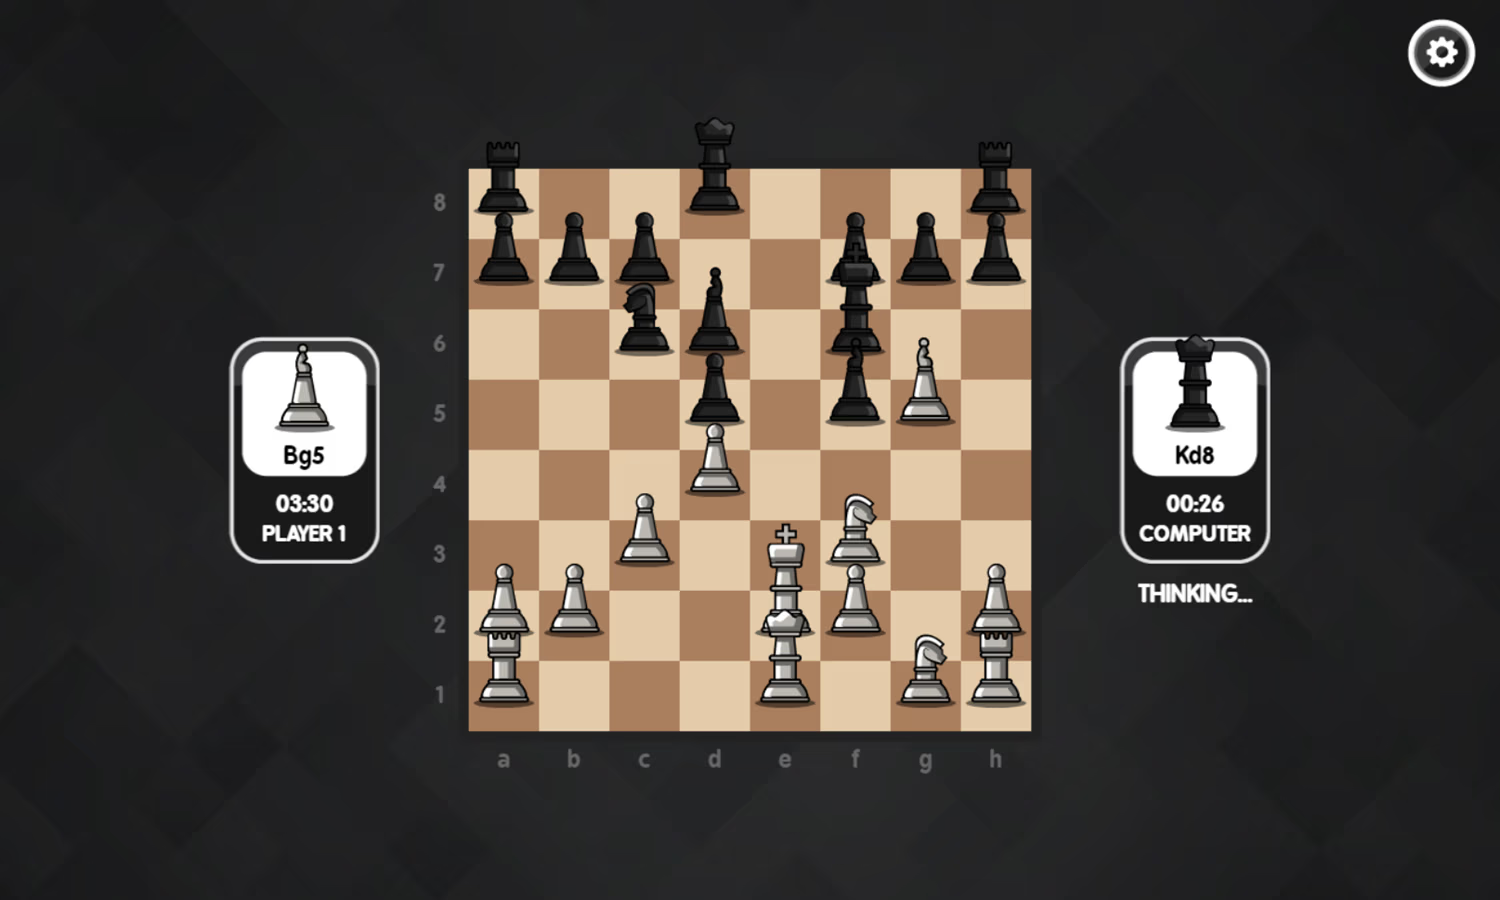
\includegraphics[width=0.68\textwidth]{Content/Giới thiệu/images/chess.png}
    \caption{Minh họa ý tưởng không gian chiến thuật và tạo hình quân cờ của Convergence Chess}
    \label{fig:intro_concept}
\end{figure}

\subsubsection{Không gian bàn cờ, đội hình và vật cản ngẫu nhiên}
Bàn cờ gồm $36$ ô được đánh chỉ số từ $0$ đến $35$ theo công thức $\text{chỉ số} = y \times 6 + x$:
\begin{itemize}
    \item \textbf{Sân nhà Người chơi 1:} Hàng 0 và hàng 1 (từ ô $0$ đến ô $11$), quân Vua đứng cố định tại ô $(3,0)$ (tương ứng ô d1).
    \item \textbf{Sân nhà Người chơi 2:} Hàng 4 và hàng 5 (từ ô $24$ đến ô $35$), quân Vua đứng cố định tại ô $(3,5)$ (tương ứng ô d6).
    \item \textbf{Vùng trung tuyến:} Hàng 2 và hàng 3 (từ ô $12$ đến ô $23$). Khi khởi tạo ván đấu, hệ thống sinh ngẫu nhiên $1$ đến $2$ ô vật cản chỉ trong vùng trung tuyến này dựa trên một hạt giống ngẫu nhiên xác định. Các quân di chuyển theo đường trượt (Xe, Tượng, Hậu) bị chặn đường bởi vật cản, trong khi quân có kỹ năng nhảy chữ L (Mã) được phép nhảy vượt qua.
    \item \textbf{Thiết lập đội hình trước trận:} Trước khi vào trận, mỗi người chơi có ngân sách hiện hành là \textbf{12 điểm đội hình} để mua và tự do sắp xếp quân cờ trong sân nhà của mình ngoài quân Vua mặc định (chi tiết chi phí và kỹ năng từng loại quân được tổng hợp tại Bảng \ref{tab:piece_roster}).
\end{itemize}

\begin{table}[H]
    \centering
    \caption{Bảng chi phí điểm đội hình, kỹ năng di chuyển gốc và kỹ năng thức tỉnh khi hợp thể}
    \label{tab:piece_roster}
    \begin{tabularx}{\textwidth}{L{2.2cm} C{1.6cm} L{2.8cm} L{2.7cm} Y}
        \toprule
        \textbf{Quân cờ} & \textbf{Chi phí (điểm)} & \textbf{Chi phí AP di chuyển} & \textbf{Kỹ năng di chuyển gốc} & \textbf{Kỹ năng thức tỉnh khi làm quân nguồn hợp thể} \\
        \midrule
        Tốt & 1 & 1 AP mỗi bước tiến hoặc ăn chéo & Không có & Cộng thêm AP: tự động hồi thêm $+1$ AP ở đầu mỗi lượt chơi. \\
        Mã & 3 & 2 AP cố định mỗi nước nhảy & Nhảy chữ L vượt vật cản và quân chắn & Phá khiên: xuyên thủng và phá hủy trực tiếp lớp khiên hộ mệnh. \\
        Tượng & 4 & 1 AP mỗi ô trượt chéo & Trượt tự do theo 4 đường chéo & Hút năng lượng chiến đấu: hoàn trả $+1$ AP ngay khi tiêu diệt 1 quân địch. \\
        Xe & 5 & 1 AP mỗi ô trượt ngang/dọc & Trượt tự do theo hàng ngang và cột dọc & Khiên hộ mệnh: tạo 1 lớp khiên chặn đòn tiêu diệt đầu tiên và đẩy lùi kẻ tấn công. \\
        Hậu & 6 (khóa mua trước trận) & 1 AP mỗi ô trượt 8 hướng & Trượt tự do theo cả 8 hướng & Rút điểm hành động: trừ $-1$ AP của đối thủ khi tiêu diệt 1 quân địch. Hiện chỉ đạt được thông qua phong cấp Tốt trong trận. \\
        Vua & Cố định & 1 AP (di chuyển 1 ô theo 8 hướng) & Không có & Không được phép tham gia hợp thể; mất Vua là thua trận. \\
        \bottomrule
    \end{tabularx}
\end{table}

\subsubsection{Kinh tế điểm hành động (AP) và cơ chế chống kéo dài trận đấu}
Thay vì cho phép mọi quân cờ di chuyển miễn phí với cự ly bất kỳ như cờ vua cổ điển, mỗi hành động trong \textit{Convergence Chess} đều tiêu hao Điểm hành động (AP) theo quy tắc cân bằng linh hoạt:
\begin{itemize}
    \item Hai bên khởi đầu với lượng AP bằng nhau ($3$ AP). Ở đầu mỗi lượt, người chơi được hồi $+2$ AP (cộng thêm $+1$ AP cho mỗi quân đang sở hữu kỹ năng cộng thêm AP), tích lũy tối đa đến ngưỡng \textbf{5 AP} và không bao giờ giảm xuống dưới $0$.
    \item Người chơi có quyền chủ động bỏ lượt để tích lũy AP cho các nước đi tầm xa hoặc hợp thể ở lượt sau, nhưng bị giới hạn tối đa $3$ lần bỏ lượt mỗi trận nhằm ngăn chặn hành vi câu giờ. Nếu tới lượt một phe không còn bất kỳ hành động hợp lệ nào (đã hết lượt bỏ lượt và không có nước đi đủ AP), hệ thống sẽ xử thua cho phe đó.
    \item Toàn bộ ván đấu bị giới hạn tối đa $60$ lượt đi lẻ; nếu đạt đến giới hạn này mà chưa có bên nào tiêu diệt được Vua đối phương, ván đấu được xử hòa.
\end{itemize}

\subsubsection{Cơ chế hợp thể quân cờ, khiên hộ mệnh và đòn bồi Surge}
Điểm sáng tạo cốt lõi tạo nên tên gọi \textit{Convergence Chess} là hệ thống hợp thể quân cờ:
\begin{enumerate}
    \item \textbf{Điều kiện và chi phí hợp thể:} Một quân đồng minh A (quân nguồn, không phải Vua) di chuyển hợp lệ vào ô của quân đồng minh B (quân đích, không phải Vua) sẽ tiêu tốn tổng AP bằng chi phí di chuyển cộng với phụ phí hợp thể (hiện được thiết lập bằng $0$ để khuyến khích nhịp độ hợp thể sớm và có thể tinh chỉnh linh hoạt khi cân bằng trò chơi). Sau khi hợp thể, quân A rời khỏi bàn cờ; quân B giữ nguyên vị trí, kế thừa kỹ năng di chuyển gốc của A và đồng thời \textbf{thức tỉnh} kỹ năng đặc biệt của A. Để bảo đảm tính cân bằng, luật áp dụng hai giới hạn cứng: không cho phép hợp thể hai quân cùng loại cơ bản ban đầu và mỗi quân cờ chỉ được tham gia hợp thể tối đa một lần trong suốt ván đấu.
    \item \textbf{Cơ chế đòn bồi (Surge):} Ngay sau khi quân B hoàn tất hợp thể, nếu người chơi vẫn còn đủ AP cho ít nhất một nước đi hoặc đòn tấn công hợp lệ từ chính quân B, hệ thống sẽ mở giai đoạn \textbf{đòn bồi (Surge)} ngay trong lượt đó. Người chơi có thể chọn tung thêm một nước đi bồi bằng quân vừa hợp thể hoặc kết thúc lượt để giữ lại AP mà \textbf{không bị trừ} số lần bỏ lượt.
    \item \textbf{Tương tác giữa Khiên hộ mệnh và Phá khiên:} Khi một quân địch không có kỹ năng Phá khiên tấn công mục tiêu đang mang Khiên hộ mệnh, lớp khiên sẽ vỡ, mục tiêu sống sót tại chỗ còn kẻ tấn công bị đẩy ngược về ô xuất phát và vẫn mất AP. Ngược lại, kẻ tấn công có kỹ năng Phá khiên sẽ xuyên qua lớp khiên và tiêu diệt mục tiêu ngay lập tức.
    \item \textbf{Phong cấp Tốt:} Khi quân Tốt tiến tới hàng cuối cùng bên sân đối phương (hàng 5 với Người chơi 1, hàng 0 với Người chơi 2), quân này lập tức tiến hóa thành Hậu, nhận thêm kỹ năng trượt 8 hướng và kỹ năng rút AP đối thủ trong khi vẫn bảo lưu các kỹ năng sẵn có.
\end{enumerate}

\subsection{Mục tiêu và phạm vi thực hiện của giai đoạn 1 (DACN)}
Đề tài được triển khai xuyên suốt hai học kỳ gồm \textbf{Giai đoạn 1 -- Đồ án chuyên ngành (DACN)} và \textbf{Giai đoạn 2 -- Đồ án tốt nghiệp (DATN)}. Trong phạm vi \textbf{DACN (Giai đoạn 1)}, mục tiêu không phải phát hành ngay bản thương mại hoàn chỉnh, mà tập trung chứng minh tính khả thi kiến trúc, khảo sát công nghệ, xây dựng nguyên mẫu chơi thử thực tế và thu thập số liệu thực nghiệm làm nền tảng cho DATN:
\begin{itemize}
    \item \textbf{Kiến trúc phần mềm:} Xây dựng phần lõi xử lý luật chơi tách rời hoàn toàn khỏi đồ họa 3D, cho phép tái sử dụng nguyên vẹn trên cả 3 chế độ chơi (đấu với máy, đấu 2 người trên cùng máy, đấu trực tuyến) và chạy mô phỏng không hiển thị đồ họa ở tốc độ cao để phục vụ huấn luyện AI.
    \item \textbf{Khảo sát và thực nghiệm AI:} Tập trung xây dựng và đánh giá định lượng hai hướng tác nhân AI chủ lực là \textbf{Hybrid Bot} (phát triển qua chuỗi thành phần nền tảng gồm tìm kiếm Minimax Alpha-Beta, học bắt chước, học tăng cường PPO \cite{mlagents} và mạng đánh giá nhanh NNUE \cite{nnue}) và \textbf{LLM Bot} (tiến hóa hàm đánh giá biểu tượng bằng Mô hình Ngôn ngữ Lớn theo hướng FunSearch \cite{funsearch}).
    \item \textbf{Khảo sát và nguyên mẫu Multiplayer:} Đánh giá các giải pháp mạng, đo đạc thực nghiệm giữa cơ chế đồng bộ đối tượng (\texttt{Fusion Network Object}) và luồng dữ liệu tin cậy (\texttt{Fusion Reliable Data Stream}), hoàn thiện nguyên mẫu phòng chơi Lobby trên \texttt{GameMode.Shared} (tạo/vào phòng, chọn region, phân vai Trắng/Đen/Khán giả, đồng bộ đội hình và nước đi 4 bytes).
    \item \textbf{Khảo sát và nguyên mẫu tùy biến nhân vật 3D (Smart Customization):} Khảo sát các phương pháp tái tạo khuôn mặt 3D từ ảnh chân dung hiện có và tự xây dựng trọn vẹn quy trình sẵn sàng thương mại hóa (loại bỏ các mô hình phi thương mại), gồm nhánh tái tạo hình học khuôn mặt 25 thông số độc lập và nhánh xử lý bề mặt da, khử bóng đối xứng, vật liệu mắt cùng 6 kiểu tóc 3D tích hợp trực tiếp vào Unity 6.
    \item \textbf{Hoàn thiện bản chơi thử:} Kết nối toàn bộ luồng trải nghiệm từ màn hình chính, màn hình xây dựng đội hình, chọn chế độ chơi đến bàn cờ 3D $6 \times 6$ với bộ quân cờ phong cách Trung cổ, hoạt họa, hiệu ứng hình ảnh và âm thanh cơ bản.
\end{itemize}

Các hạng mục mang tính sản phẩm hóa và vận hành công khai như hệ thống đăng nhập tài khoản (Google/Facebook), lưu trữ đám mây, tự động ghép trận theo điểm xếp hạng Elo, hệ thống bạn bè, xử lý khôi phục kết nối nâng cao, hoàn thiện xử lý hết giờ/đầu hàng/cài đặt âm thanh và thử nghiệm người dùng quy mô lớn được quy hoạch rõ ràng sang \textbf{Giai đoạn 2 (DATN)}.

\subsection{So sánh với các sản phẩm tương tự và đánh giá ưu, nhược điểm của thiết kế lối chơi}
Bảng \ref{tab:market_comparison} đối chiếu \textit{Convergence Chess} với ba đại diện tiêu biểu trên thị trường nhằm làm rõ giá trị khác biệt của đề tài.

\begin{table}[H]
    \centering
    \caption{So sánh Convergence Chess với các trò chơi chiến thuật cờ tương tự}
    \label{tab:market_comparison}
    \begin{tabularx}{\textwidth}{L{2.8cm} Y Y Y Y}
        \toprule
        \textbf{Tiêu chí} & \textbf{Cờ vua truyền thống (Chess.com / Lichess)} & \textbf{Shotgun King / Pawnbarian} & \textbf{Teamfight Tactics} & \textbf{Convergence Chess} \\
        \midrule
        Kích thước và địa hình & Bàn $8 \times 8$ phẳng, cố định & Bàn $8 \times 8$ hoặc lưới nhỏ biến đổi theo màn & Bàn lưới lục giác, không vật cản địa hình & Bàn $6 \times 6$ kèm $1$--$2$ ô vật cản sinh ngẫu nhiên ở trung tuyến \\
        Cơ chế tài nguyên & Không có điểm hành động; mỗi lượt đi 1 quân & Tài nguyên đạn hoặc thẻ bài theo lượt & Kinh tế vàng mua tướng & Kinh tế điểm hành động tích lũy ($+2$/lượt, tối đa $5$), giới hạn số lần bỏ lượt \\
        Tùy biến đội hình và nâng cấp & Đội hình 16 quân cố định, chỉ phong Tốt & Nâng cấp ngẫu nhiên giữa các màn & Ghép 3 tướng giống nhau tăng cấp & Tự xây dựng đội hình (12 điểm) và hợp thể quân khác loại để thức tỉnh kỹ năng kèm đòn bồi Surge \\
        Chế độ chơi và AI & Đấu trực tuyến kèm máy đánh cờ Stockfish/Leela & Chủ yếu chơi đơn với máy & Đấu trực tuyến 8 người & Đấu với máy (Hybrid Bot và LLM Bot), đấu 2 người cùng máy và đấu trực tuyến \\
        Cá nhân hóa 3D & Bộ cờ 2D/3D có sẵn & Đồ họa điểm ảnh 2D & Linh thú bán sẵn & Thử nghiệm tạo nhân vật 3D từ ảnh chân dung (Smart Customization) \\
        \bottomrule
    \end{tabularx}
\end{table}

Bên cạnh giá trị khác biệt, thiết kế lối chơi của \textit{Convergence Chess} cũng đi kèm những ưu điểm và đánh đổi rõ rệt:
\begin{itemize}
    \item \textbf{Ưu điểm:} Bàn cờ $6 \times 6$ rút ngắn thời gian mỗi ván đấu và đẩy nhanh nhịp độ giao tranh ngay từ các lượt đầu; cơ chế tự chọn đội hình kết hợp hợp thể khác loại và đòn bồi Surge tạo ra không gian chiến thuật phong phú, hạn chế tình trạng học thuộc khai cuộc; vật cản sinh ngẫu nhiên ở trung tuyến giúp mỗi ván đấu mang tính biến hóa cao.
    \item \textbf{Nhược điểm và thách thức:} Nhiều cơ chế mới chồng lên nhau (kinh tế điểm hành động, $9$ kỹ năng nội tại gồm di chuyển và thức tỉnh, khóa hợp thể, đòn bồi Surge) tạo rào cản tiếp cận ban đầu cao hơn cờ vua truyền thống đối với người chơi mới; không gian $6 \times 6$ hẹp hơn nên dễ xảy ra tình trạng mất cân bằng lợi thế đi trước/đi sau nếu bộ tham số điểm hành động và chi phí đội hình chưa được hiệu chỉnh qua mô phỏng số lượng lớn.
\end{itemize}

\subsection{Phân công trách nhiệm trong nhóm thực hiện}
Dự án được thực hiện bởi 2 thành viên với ranh giới phân hệ rõ ràng, kết nối với nhau qua các giao diện trao đổi dữ liệu thống nhất:
\begin{itemize}
    \item \textbf{Thành viên 1 (Chủ trì Lõi luật chơi, AI và Smart Customization):} Thiết kế kiến trúc tổng thể tách biệt lõi và giao diện; xây dựng toàn bộ lõi luật chơi $6 \times 6$ (trạng thái bàn cờ, kiểm định nước đi, điều phối vòng lặp trận đấu và cấu hình cân bằng); xây dựng hai dòng tác nhân AI chính là \textbf{Hybrid Bot} (cùng chuỗi thành phần Minimax, học bắt chước, học tăng cường PPO, mạng đánh giá NNUE) và \textbf{LLM Bot}; phát triển quy trình tạo nhân vật 3D từ ảnh chân dung (Smart Customization) và cơ chế đồng bộ sự kiện hoạt họa quân cờ.
    \item \textbf{Thành viên 2 -- Đăng (Chủ trì Multiplayer và View Layer):} Khảo sát và hiện thực hệ thống Multiplayer trên nền tảng Photon Fusion (\texttt{OnlineSessionManager}, \texttt{OnlineDataBroadcastNetwork}, \texttt{NetworkController}, \texttt{PvPOnlModeBootstrapper}, đo benchmark mạng), chế độ PvP Offline (\texttt{BoardRotator}), tầng hiển thị bàn cờ và quân cờ 3D, toàn bộ hệ thống giao diện người dùng (màn hình chính, xây dựng đội hình, sảnh chờ trực tuyến, bảng thông số trong trận) và tích hợp hiệu ứng hình ảnh, âm thanh, bối cảnh 3D.
\end{itemize}

\newpage
\section{Yêu cầu của đề tài}

\subsection{Các bên liên quan và câu chuyện người dùng}
Để bảo đảm hệ thống đáp ứng đúng cả góc độ trải nghiệm người chơi lẫn yêu cầu nghiên cứu AI và Multiplayer của một đồ án chuyên ngành, nhóm xác định bốn nhóm đối tượng liên quan chính:
\begin{itemize}
    \item \textbf{Người chơi:} Đối tượng trực tiếp xây dựng đội hình, trải nghiệm các chế độ đấu với máy, đấu hai người trên cùng máy, đấu trực tuyến và tùy biến nhân vật 3D.
    \item \textbf{Khán giả:} Người tham gia phòng trực tuyến ở vai trò quan sát trực tiếp diễn biến ván đấu của hai người chơi chính mà không can thiệp vào luồng điều khiển.
    \item \textbf{Nhóm phát triển và nghiên cứu AI:} Sử dụng chính lõi trò chơi ở chế độ mô phỏng không hiển thị đồ họa để chạy hàng nghìn ván đấu tự động, huấn luyện các thành phần của Hybrid Bot và LLM Bot cũng như thu thập số liệu đánh giá.
    \item \textbf{Giảng viên hướng dẫn và Hội đồng đánh giá:} Đánh giá tính đúng đắn của kiến trúc, mức độ hoàn thiện của nguyên mẫu giai đoạn 1 và độ tin cậy của các kết quả thực nghiệm.
\end{itemize}

Bảng \ref{tab:user_stories} tổng hợp các câu chuyện người dùng cốt lõi làm đầu vào cho việc đặc tả yêu cầu chức năng và lược đồ ca sử dụng (Use-case) ở Chương 4.

\begin{table}[H]
    \centering
    \caption{Danh sách câu chuyện người dùng cốt lõi của hệ thống Convergence Chess}
    \label{tab:user_stories}
    \begin{tabularx}{\textwidth}{C{1.3cm} L{2.4cm} Y C{2.0cm}}
        \toprule
        \textbf{Mã} & \textbf{Vai trò} & \textbf{Nội dung nhu cầu người dùng} & \textbf{Ưu tiên} \\
        \midrule
        US-01 & Người chơi & Tôi muốn tự chọn và sắp xếp quân cờ trong ngân sách 12 điểm đội hình tại màn hình chính và lưu lại để sử dụng ngay khi vào trận. & Cao \\
        US-02 & Người chơi & Tôi muốn khi chọn một quân cờ trên bàn $6 \times 6$, hệ thống tự động tô sáng rõ các ô di chuyển, tấn công và hợp thể hợp lệ kèm bảng thông tin quân cờ. & Cao \\
        US-03 & Người chơi & Tôi muốn thực hiện hợp thể hai quân cờ khác loại để thức tỉnh kỹ năng đặc biệt mới và tung đòn bồi trong giai đoạn Surge nếu còn đủ điểm hành động. & Cao \\
        US-04 & Người chơi & Tôi muốn đấu với máy thông qua các tác nhân AI có chiều sâu chiến thuật (Hybrid Bot và LLM Bot) để luyện tập. & Cao \\
        US-05 & Người chơi & Tôi muốn đấu PvP Offline với bạn bè trên cùng một máy và bàn cờ tự xoay góc nhìn sau mỗi lượt chơi. & Trung bình \\
        US-06 & Người chơi & Tôi muốn chọn khu vực máy chủ (Region), tạo phòng Online bằng mã phòng, đồng bộ đội hình với đối thủ và thi đấu trực tuyến ổn định. & Cao \\
        US-07 & Khán giả & Tôi muốn tham gia phòng Online ở vị trí Spectator để theo dõi diễn biến từng nước đi theo thời gian thực mà không làm ảnh hưởng đến trận đấu. & Trung bình \\
        US-08 & Người chơi & Tôi muốn tải lên ảnh chân dung 2D để hệ thống tự tái tạo hình học khuôn mặt, màu da, màu mắt và cho phép thay đổi kiểu tóc 3D trong trò chơi. & Trung bình \\
        US-09 & Nhà nghiên cứu & Tôi muốn khởi chạy nhiều bàn cờ song song ở chế độ không hiển thị đồ họa và tự động ghi nhận tỷ lệ thắng cùng thời gian suy nghĩ của các mô hình AI để phân tích. & Cao \\
        \bottomrule
    \end{tabularx}
\end{table}

\subsection{Yêu cầu chức năng}
Các yêu cầu chức năng được phân tách thành năm nhóm lớn tương ứng với các phân hệ chính của dự án:

\subsubsection{Nhóm chức năng thiết lập đội hình và vòng lặp lối chơi cốt lõi}
\begin{itemize}
    \item \textbf{FR-01 (Quản lý đội hình):} Cung cấp màn hình xây dựng đội hình cho phép kéo thả hoặc đặt quân cờ vào 12 ô sân nhà (ngoại trừ ô Vua đứng cố định), tự động kiểm tra ràng buộc ngân sách 12 điểm đội hình và danh sách quân cờ được phép sử dụng, đồng thời lưu trữ cấu hình đội hình trên máy để tái sử dụng cho các trận sau.
    \item \textbf{FR-02 (Khởi tạo bàn cờ và vật cản):} Tự động nạp đội hình hai bên, đặt hai quân Vua tại vị trí cố định và sinh ngẫu nhiên $1$--$2$ ô vật cản tại vùng trung tuyến (hàng 2 và hàng 3) theo hạt giống ngẫu nhiên xác định.
    \item \textbf{FR-03 (Thẩm định và thực thi nước đi):} Kiểm tra chính xác tính hợp lệ của nước di chuyển, tấn công, vượt vật cản, hợp thể (áp dụng khóa cấm hợp thể cùng loại và khóa mỗi quân chỉ hợp thể một lần), phong cấp Tốt, tương tác Khiên hộ mệnh với Phá khiên, cộng trừ điểm hành động và kích hoạt giai đoạn đòn bồi Surge.
    \item \textbf{FR-04 (Điều kiện kết thúc và bỏ lượt):} Hỗ trợ hành động bỏ lượt có giới hạn tối đa $3$ lần mỗi trận, tự động kết thúc trận khi Vua bị tiêu diệt, xử thua khi phe tới lượt không còn hành động hợp lệ nào hoặc xử hòa khi vượt quá giới hạn $60$ lượt đi lẻ. Tính năng đầu hàng đã được chuẩn bị ở tầng giao thức mạng và sẽ nối hoàn chỉnh lên giao diện ở Giai đoạn 2.
\end{itemize}

\subsubsection{Nhóm chức năng trí tuệ nhân tạo và đánh giá đối kháng}
\begin{itemize}
    \item \textbf{FR-05 (Hỗ trợ hai dòng tác nhân AI chính):} Cho phép gắn linh hoạt hai dòng tác nhân AI chính là \textbf{Hybrid Bot} (kết hợp tìm kiếm cây trò chơi, học tăng cường PPO và mạng đánh giá nhanh NNUE) và \textbf{LLM Bot} (đánh giá thế cờ bằng tập luật biểu tượng tiến hóa từ Mô hình Ngôn ngữ Lớn) vào vị trí Người chơi 1 hoặc Người chơi 2 thông qua cùng một giao diện nhận nước đi thống nhất.
    \item \textbf{FR-06 (Hạ tầng huấn luyện và đối kháng tự động):} Cung cấp môi trường mô phỏng chuyên biệt phục vụ thu thập dữ liệu chuyên gia, huấn luyện tự đấu đa bàn cờ song song và tự động ghi nhận kết quả đối kháng (tỷ lệ thắng, thua, hòa và thời gian trung bình mỗi nước đi).
\end{itemize}

\subsubsection{Nhóm chức năng nhiều người chơi (PvP Offline và PvP Online)}
\begin{itemize}
    \item \textbf{FR-07 (Chế độ PvP Offline):} Hai người chơi thao tác luân phiên trên cùng thiết bị, hỗ trợ nạp đội hình độc lập cho từng bên và tự động xoay bàn cờ $180^\circ$ sau mỗi lượt bằng \texttt{BoardRotator}.
    \item \textbf{FR-08 (Quản lý phòng Online và phân vai):} Cho phép chọn khu vực máy chủ Photon, nhập mã phòng để tạo hoặc tham gia phiên chơi (\texttt{GameMode.Shared}), đổi vị trí giữa 3 vai trò (Trắng, Đen, Khán giả), đồng bộ tên người chơi, trạng thái sẵn sàng và đội hình hai bên.
    \item \textbf{FR-09 (Đồng bộ trận đấu Online):} Khi trận bắt đầu, máy chủ phòng (Host -- Shared Mode Master Client) phát tán đồng bộ hạt giống vật cản và đội hình (\texttt{MSG\_MATCH\_INIT}); trong trận, mọi lệnh di chuyển và bỏ lượt được truyền tin cậy dưới dạng gói nhị phân cố định 4 bytes (\texttt{MSG\_MOVE}) kèm bộ đếm thời gian lượt đi \texttt{OnlineTurnTimer} (60 giây/lượt; luồng tự động xử lý khi hết giờ \texttt{OnTimerExpired} và nút đầu hàng sẽ nối mạch hoàn chỉnh ở Giai đoạn 2).
\end{itemize}

\subsubsection{Nhóm chức năng tầng hiển thị, giao diện và âm thanh}
\begin{itemize}
    \item \textbf{FR-10 (Diễn hoạt tách rời logic):} Toàn bộ các sự kiện thay đổi trạng thái trong một nước đi được gom thành từng đợt và đưa vào hàng đợi trực quan để phát tuần tự hoạt họa 3D, hiệu ứng rung hoặc phóng cận cảnh góc quay, hiệu ứng va chạm và âm thanh mà không làm gián đoạn luồng xử lý luật chơi.
    \item \textbf{FR-11 (Bảng thông số trong trận và cài đặt):} Hiển thị trực quan lượng điểm hành động hiện có, lượng điểm dự kiến hồi ở lượt sau, số lượt bỏ lượt còn lại, lượt đi hiện tại, danh sách quân cờ đã bị tiêu diệt và hộp thoại cài đặt (Giai đoạn 1 đã hoàn thiện mục cài đặt chung lưu tên người chơi; các mục âm thanh, đồ họa và phím điều khiển đã dựng sẵn khung giao diện để mở rộng ở Giai đoạn 2).
\end{itemize}

\subsubsection{Nhóm chức năng mở rộng tùy biến nhân vật 3D (Smart Customization)}
\begin{itemize}
    \item \textbf{FR-12 (Tái tạo khuôn mặt và tóc 3D từ ảnh 2D):} Cho phép người dùng chọn ảnh chân dung 2D và giới tính (Nam/Nữ) trực tiếp trên giao diện trong game; hệ thống gọi mô-đun suy luận AI cục bộ để phân tích ảnh, sau đó tự động áp $25$ thông số hình thái khuôn mặt, kết cấu da đã khử bóng, bản đồ chi tiết bề mặt, màu mắt và màu tóc lên nhân vật 3D; đồng thời hỗ trợ người chơi tinh chỉnh thủ công bằng thanh trượt và chuyển đổi giữa 7 lựa chọn kiểu tóc 3D (6 mẫu tóc 3D và chế độ không tóc).
\end{itemize}

\subsection{Yêu cầu phi chức năng}
\begin{itemize}
    \item \textbf{Tính tách biệt và khả năng bảo trì:} Phần lõi quy tắc và trạng thái bàn cờ phải tách hoàn toàn khỏi đồ họa 3D, chỉ đọc tham số cân bằng từ nguồn cấu hình tập trung, bảo đảm cùng một trạng thái bàn cờ và cùng một nước đi luôn cho ra kết quả giống hệt nhau trên mọi máy người chơi cũng như trong môi trường huấn luyện AI.
    \item \textbf{Hiệu năng tính toán:}
    \begin{itemize}
        \item Chế độ chơi thực tế duy trì tốc độ khung hình ổn định từ $60$ khung hình/giây trở lên trên máy tính cá nhân tầm trung (cạc đồ họa RTX 4050 Laptop).
        \item Thời gian phản hồi trung bình của tác nhân AI trong trận đấu thực tế dưới $0.5$ giây mỗi nước đi (mục tiêu dưới $100$ mili-giây đối với thành phần đánh giá nhanh ở độ sâu 4).
        \item Chế độ mô phỏng không hiển thị đồ họa cho phép chạy hàng trăm ván đấu trong vài chục giây mà không gây rò rỉ bộ nhớ.
    \end{itemize}
    \item \textbf{Hiệu quả băng thông mạng (Network Efficiency):} Tối ưu kích thước gói tin đồng bộ nước đi xuống mức tối thiểu (dưới $100$ bytes cho chuỗi 10 lần thăm dò) để bảo đảm tính ổn định kể cả trên đường truyền mạng thông thường.
    \item \textbf{Thời gian xử lý tùy biến nhân vật 3D:} Toàn bộ quy trình phân tích ảnh chân dung 2D, giải hình học khuôn mặt, chiếu kết cấu và khử bóng da trên máy tính cục bộ cần hoàn tất trong vài giây (thực tế đo được khoảng $5.9$ giây mỗi ảnh) để người chơi xem trước thuận tiện ngay trong game.
\end{itemize}

\subsection{Yêu cầu kỹ thuật và trải nghiệm người dùng}
\begin{itemize}
    \item \textbf{Nền tảng mục tiêu:} Hệ điều hành Windows (ứng dụng PC 64-bit), xây dựng trên nền tảng Unity 6 \cite{unity6} với ngôn ngữ C\# kết hợp môi trường Python (PyTorch, PyTorch3D \cite{pytorch3d}, ONNX Runtime, MediaPipe \cite{mediapipe}) phục vụ huấn luyện AI và quy trình tái tạo nhân vật 3D cục bộ.
    \item \textbf{Trải nghiệm người dùng:} Cung cấp phản hồi hình ảnh và âm thanh tức thời khi di chuột qua ô cờ, chọn quân, di chuyển, va chạm khiên hoặc hợp thể; bố cục giao diện tự co giãn theo độ phân giải màn hình và trình bày rõ ràng trạng thái điểm hành động để giảm bớt độ phức tạp cho người mới làm quen với luật hợp thể.
\end{itemize}

\newpage
\section{Nghiên cứu tổng quan và cơ sở lý thuyết}

\subsection{Quy trình phát triển phần mềm và công cụ quản lý dự án}
Do đặc thù của đề tài kết hợp đồng thời phát triển trò chơi 3D, thử nghiệm mạng trực tuyến và nghiên cứu nhiều kỹ thuật học máy có độ bất định cao, nhóm áp dụng quy trình phát triển lặp tăng trưởng theo tinh thần \textbf{Agile} với chu kỳ kiểm nghiệm theo tuần (15 tuần cho Giai đoạn 1). Khác với mô hình thác nước đòi hỏi khóa cứng toàn bộ đặc tả từ đầu, cách tiếp cận lặp cho phép nhóm nhanh chóng điều chỉnh tham số cân bằng điểm hành động và hợp thể, chuyển đổi giải pháp mạng từ Unity NGO sang Photon Fusion dựa trên số liệu đo đạc thực tế, và cải tiến liên tục hai hướng tác nhân AI là Hybrid Bot và LLM Bot.

Các công cụ hỗ trợ quản lý và triển khai gồm:
\begin{itemize}
    \item \textbf{Git và GitHub:} Quản lý phiên bản mã nguồn phân nhánh độc lập theo vai trò giữa hai thành viên, giúp theo dõi lịch sử thay đổi xuyên suốt giai đoạn 1 và hạn chế xung đột trên các tài nguyên đồ họa Unity.
    \item \textbf{Unity 6:} Được lựa chọn so với Unreal Engine và Godot nhờ cân bằng tốt giữa năng suất lập trình C\# (thuận lợi cho việc tách riêng lõi luật chơi không phụ thuộc đồ họa), hệ sinh thái gói chính chủ \textbf{Unity ML-Agents} \cite{mlagents}, khả năng tích hợp mượt mà với \textbf{Photon Fusion 2} \cite{photon_fusion} và trình kết xuất đồ họa nhẹ phù hợp với phần cứng máy tính tầm trung (bộ nhớ đồ họa 6 GB) \cite{unity6}.
    \item \textbf{Python, PyTorch, ONNX Runtime và Blender 4.2 (MPFB v2):} Hệ sinh thái tiêu chuẩn để huấn luyện các mô hình học máy cho Hybrid Bot, chạy vòng lặp tiến hóa luật cho LLM Bot bằng Gemini API và xây dựng quy trình tái tạo khuôn mặt cùng tóc 3D cho Smart Customization \cite{mpfb2}.
\end{itemize}

\subsection{Các nguyên tắc và mẫu thiết kế kiến trúc áp dụng}
Để giữ cấu trúc phần mềm gọn gàng và dễ mở rộng trong suốt hai giai đoạn thực hiện, hệ thống vận dụng có chọn lọc năm mẫu thiết kế kiến trúc sau:
\begin{itemize}
    \item \textbf{Kiến trúc lục giác tách biệt lõi và giao diện \cite{cockburn}:} Đặt toàn bộ thực thể và quy tắc cờ trong vùng lõi độc lập khỏi đồ họa 3D. Mọi tương tác vào ra của ván đấu đều đi qua hai cổng giao tiếp chuẩn: một cổng tiếp nhận nước đi (từ người chơi, từ mạng hoặc từ AI) và một cổng phát sự kiện diễn biến ván đấu cho phần hiển thị hoặc bộ ghi nhận thực nghiệm.
    \item \textbf{Cô lập dịch vụ theo từng bàn đấu:} Thay vì dùng biến dùng chung toàn cục dễ gây xung đột khi chạy song song nhiều bàn cờ huấn luyện AI, mỗi bàn đấu sở hữu một vùng quản lý dịch vụ riêng được cấu hình độc lập tùy theo chế độ chơi (đấu với máy, đấu hai người hay chạy mô phỏng huấn luyện).
    \item \textbf{Chuẩn hóa lệnh hành động và gom nhóm sự kiện:} Mọi nước đi đều được đóng gói thành một cấu trúc lệnh thống nhất; sau khi lõi luật xử lý xong sẽ phát ra một gói sự kiện theo đúng trình tự xảy ra, giúp tầng hiển thị diễn hoạt tuần tự còn các bộ theo dõi huấn luyện vẫn lắng nghe độc lập.
    \item \textbf{Máy trạng thái hữu hạn cho hoạt họa quân cờ:} Quản lý rõ ràng 5 trạng thái hoạt họa của từng quân cờ 3D (đứng chờ, di chuyển, tấn công, bị đánh trúng và bị tiêu diệt), giúp mã xử lý hoạt họa gọn gàng và dễ mở rộng thêm mẫu quân cờ mới.
    \item \textbf{Mẫu thiết kế khởi tạo theo loại bản tin và bọc bộ điều khiển trong tầng mạng:} Áp dụng cho phân hệ Multiplayer để tự động phân tuyến gói tin nhị phân theo mã định danh và bổ sung tính năng gửi nước đi lên mạng mà không cần sửa đổi bộ điều khiển chuột cục bộ.
\end{itemize}

\subsection{Cơ sở lý thuyết và đánh giá giải pháp Networking}
\subsubsection{So sánh các giải pháp Networking cho Unity}
Trong giai đoạn phác thảo đề cương ban đầu, nhóm từng cân nhắc Unity Netcode for GameObjects (NGO). Tuy nhiên, khi đi vào phân tích kiến trúc cụ thể của \textit{Convergence Chess} (lõi luật tách rời \texttt{GameObject}, lối chơi theo lượt cần độ tin cậy tuyệt đối và không muốn phụ thuộc vào hạ tầng cấu hình Relay/Lobby phức tạp), nhóm đã khảo sát và so sánh ba giải pháp phổ biến trong hệ sinh thái Unity như Bảng \ref{tab:net_solutions}.

\begin{table}[H]
    \centering
    \caption{So sánh các giải pháp Networking cho game chiến thuật theo lượt trên Unity}
    \label{tab:net_solutions}
    \begin{tabularx}{\textwidth}{L{2.5cm} Y Y Y}
        \toprule
        \textbf{Tiêu chí} & \textbf{Unity NGO} & \textbf{Mirror Networking} & \textbf{Photon Fusion 2} \\
        \midrule
        Hạ tầng kết nối & Cần tích hợp thêm Unity Lobby và Unity Relay để vượt NAT & Tự quản lý máy chủ hoặc dùng Transport trung gian (KCP/Telepathy) & Tích hợp sẵn Photon Cloud toàn cầu, chọn Region trực tiếp, không cần dựng server riêng \\
        Mức độ phụ thuộc GameObject & Mạnh (yêu cầu gắn \texttt{NetworkObject} và \texttt{NetworkBehaviour}) & Mạnh (yêu cầu \texttt{NetworkIdentity} trên các đối tượng đồng bộ) & Hỗ trợ cả \texttt{NetworkObject} lẫn truyền luồng byte thuần qua \texttt{SendReliableDataToPlayer} \\
        Phù hợp với Core tách đồ họa & Khó tách rời nếu dùng đồng bộ đối tượng & Cần tự xây lớp cầu nối & Rất cao nhờ cơ chế \texttt{ReliableData} gửi trực tiếp struct/byte payload \\
        Chi phí giai đoạn phát triển & Miễn phí theo hạn mức Unity Gaming Services & Mã nguồn mở miễn phí (tự tốn chi phí thuê VPS/Server) & Miễn phí gói phát triển lên đến 20 CCU trên Photon Cloud \\
        \bottomrule
    \end{tabularx}
\end{table}

\textbf{Kết luận lựa chọn giai đoạn 1:} Nhóm quyết định chuyển từ Unity NGO sang \textbf{Photon Fusion 2} \cite{photon_fusion} (chạy thống nhất ở mô hình \texttt{GameMode.Shared} trên Photon Cloud, trong đó máy chủ phòng là Shared Mode Master Client) và đặc biệt chọn cơ chế truyền luồng dữ liệu tin cậy \textbf{Fusion Reliable Data Stream} thay cho đồng bộ trạng thái quân cờ bằng \texttt{Fusion Network Object}. Lựa chọn này giải quyết đồng thời hai yêu cầu sống còn: (i) cho phép triển khai nhanh chế độ PvP Online đa khu vực mà không phải vận hành máy chủ riêng ở giai đoạn DACN; và (ii) bảo toàn kiến trúc Decoupled Core vì các quân cờ trên bàn không bị biến thành \texttt{NetworkObject}. Số liệu đo đạc thực nghiệm so sánh trực tiếp giữa \texttt{Fusion Network Object} và \texttt{Fusion Reliable Data} sẽ được trình bày chi tiết tại Chương 5 và Chương 6.

\subsection{Cơ sở lý thuyết về trí tuệ nhân tạo trong game chiến thuật}
Bàn cờ $6 \times 6$ của \textit{Convergence Chess} có số ô ít hơn cờ vua $8 \times 8$, nhưng độ phức tạp rẽ nhánh lại mang nét đặc thù do tổ hợp 9 kỹ năng nội tại, kinh tế điểm hành động biến thiên theo khoảng cách di chuyển, cơ chế hợp thể và chuỗi đòn bồi Surge. Vì vậy, để xây dựng hai dòng tác nhân chính là \textbf{Hybrid Bot} và \textbf{LLM Bot}, nhóm nghiên cứu bốn nền tảng lý thuyết bổ trợ cho nhau:

\subsubsection{Tìm kiếm cây trò chơi Minimax với cắt tỉa Alpha-Beta và bảng băm Zobrist}
Thuật toán Minimax tìm nước đi tối ưu trong trò chơi đối kháng hai người theo nguyên lý cực đại hóa lợi thế trong kịch bản đối thủ phản ứng tốt nhất. Để giảm mạnh số trạng thái phải duyệt, nền tảng tìm kiếm của Hybrid Bot kết hợp các kỹ thuật tối ưu kinh điển:
\begin{itemize}
    \item \textbf{Cắt tỉa Alpha-Beta kết hợp sắp xếp nước đi ưu tiên:} Loại bỏ sớm các nhánh chắc chắn không cải thiện kết quả, đồng thời ghi nhớ các nước đi thường gây cắt tỉa tốt và bảng điểm lịch sử cho các nước đi tĩnh để duyệt những nhánh hứa hẹn trước.
    \item \textbf{Bảng hoán vị Zobrist và gia hạn độ sâu khi có đòn bồi Surge:} Mã hóa toàn bộ trạng thái bàn cờ (vị trí quân, vật cản, kỹ năng, trạng thái hợp thể, AP hai bên, số lượt bỏ lượt, trạng thái Surge và lượt đi) thành một mã băm 64-bit để tránh tính lại các thế cờ lặp. Đồng thời, hệ thống gia hạn thêm tối đa $2$ tầng tìm kiếm trên các nhánh kích hoạt đòn bồi Surge nhằm tránh hiện tượng bỏ sót đòn ăn quân liên hoàn ở rìa độ sâu tìm kiếm.
    \item \textbf{Giảm độ sâu thăm dò có kiểm chứng lại theo mạng chính sách:} Khi kết hợp với mạng nơ-ron gợi ý nước đi, bộ tìm kiếm duyệt đủ độ sâu cho nước đi tốt nhất từ bảng hoán vị, nhóm nước đi có xác suất cao và toàn bộ nước ăn quân hoặc hợp thể; với các nước đi tĩnh ít tiềm năng hơn, hệ thống duyệt nông hơn để tiết kiệm thời gian và tự động kiểm chứng lại ở độ sâu đầy đủ nếu phát hiện điểm số vượt trội.
\end{itemize}

\subsubsection{Học bắt chước và Học tăng cường PPO tự đấu (thành phần huấn luyện Hybrid Bot)}
Huấn luyện học tăng cường từ con số không trên trò chơi có tín hiệu thưởng thưa (chỉ phân định thắng thua khi tiêu diệt Vua) thường hội tụ rất chậm. Do đó, mạng chính sách của Hybrid Bot được huấn luyện qua hai bước nối tiếp trên nền tảng \textbf{Unity ML-Agents} \cite{mlagents}:
\begin{itemize}
    \item \textbf{Học bắt chước (Behavioral Cloning và DAgger \cite{dagger}):} Thu thập hàng chục nghìn cặp thế cờ và nước đi mẫu từ bộ tìm kiếm Minimax độ sâu 4 (kết hợp lấy mẫu có độ ngẫu nhiên để đa dạng hóa thế cờ và lấy nhãn tối ưu) nhằm khởi tạo trọng số mạng nơ-ron ban đầu, tránh giai đoạn mò mẫm kém hiệu quả.
    \item \textbf{Học tăng cường tối ưu chính sách cắt ngưỡng (PPO) \cite{ppo}:} Tinh chỉnh chính sách chọn nước đi $\pi_\theta(a|s)$ thông qua quá trình tự đấu bằng hàm mục tiêu cắt ngưỡng, ngăn bước cập nhật quá lớn làm sụp đổ chiến thuật đã học:
    \begin{equation}
        L^{\text{CLIP}}(\theta) = \hat{\mathbb{E}}_t \left[ \min\left( r_t(\theta)\hat{A}_t,\; \text{clip}\left(r_t(\theta), 1-\epsilon, 1+\epsilon\right)\hat{A}_t \right) \right]
    \end{equation}
    trong đó $r_t(\theta) = \frac{\pi_\theta(a_t|s_t)}{\pi_{\theta_{\text{old}}}(a_t|s_t)}$ là tỷ số xác suất giữa chính sách mới và cũ, còn $\hat{A}_t$ là ước lượng mức độ lợi thế của hành động.
    \item \textbf{Định hình phần thưởng theo hàm thế năng \cite{potential_shaping}:} Để cung cấp tín hiệu dẫn hướng đều đặn hơn trong trận mà không làm lệch mục tiêu thắng thua gốc, phần thưởng trung gian được tính từ chênh lệch điểm đánh giá thế cờ của mạng NNUE:
    \begin{equation}
        F(s_t, s_{t+1}) = \lambda \cdot \left( \gamma \Phi_{\text{NNUE}}(s_{t+1}, p) - \Phi_{\text{NNUE}}(s_t, p) \right)
    \end{equation}
\end{itemize}

\subsubsection{Mạng đánh giá nhanh NNUE và biến thể dạng dư (Residual NNUE)}
Lấy cảm hứng từ kiến trúc \textbf{NNUE} trong máy đánh cờ Stockfish \cite{nnue}, thay vì chạy suy luận mạng nơ-ron nặng ở từng nút lá của cây tìm kiếm, nhóm sử dụng một mạng nơ-ron gọn ba tầng ($654 \to 128 \to 64 \to 1$) tận dụng tính thưa của bàn cờ $6 \times 6$: chỉ cộng dồn trọng số tại những ô thực sự có quân cờ hoặc vật cản và bỏ qua toàn bộ ô trống. Ở biến thể \textbf{NNUE dạng dư (Residual NNUE)}, hệ thống giữ lại điểm đánh giá vật chất cơ sở làm mốc neo và chỉ để mạng nơ-ron học phần hiệu chỉnh chiến thuật tinh tế trong biên độ giới hạn $[-3.0, +3.0]$. Cách làm này giúp tránh sai lệch nghiêm trọng về giá trị quân cờ và tăng tốc độ hội tụ rõ rệt.

\subsubsection{Tiến hóa hàm đánh giá biểu tượng bằng Mô hình Ngôn ngữ Lớn (nền tảng LLM Bot)}
Song song với hướng học sâu của Hybrid Bot, nhóm nghiên cứu hướng \textbf{LLM Bot} theo phương pháp \textbf{FunSearch} \cite{funsearch} nhằm tạo ra tri thức chiến thuật có thể đọc hiểu và kiểm chứng được. Hệ thống sử dụng Gemini API để sinh và tiến hóa trực tiếp các đoạn quy tắc đánh giá ngắn gọn, phân loại theo 8 tình huống chiến thuật của ván đấu (khai cuộc chưa hợp thể, trung cuộc đã hợp thể, tàn cuộc ít quân, tranh chấp khiên, Vua bị đe dọa, đua phong cấp Tốt, dự trữ AP cao...). Mỗi quy tắc sinh ra đều trải qua 4 bước sàng lọc tự động về tính hợp lệ, tốc độ, tính đối xứng và tỷ lệ thắng đối kháng trước khi được lưu vào ngân hàng luật của LLM Bot.

\subsection{Cơ sở lý thuyết cho phân hệ tùy biến nhân vật 3D (Smart Customization)}
Bài toán tái tạo nhân vật 3D có sẵn khung xương để hoạt họa từ một bức ảnh chân dung 2D đơn lẻ đòi hỏi giải quyết đồng thời hai bài toán con:
\begin{itemize}
    \item \textbf{Tái tạo hình học khuôn mặt 3D:} Sử dụng \textbf{MediaPipe} \cite{mediapipe} trích xuất 478 điểm mốc giải phẫu trên ảnh 2D, sau đó ánh xạ sang hệ thống thông số biến dạng khuôn mặt của bộ khung chuẩn giải phẫu \textbf{MPFB v2} trên Blender \cite{mpfb2}. Thực nghiệm cho thấy việc dùng trực tiếp chiều sâu ước lượng từ MediaPipe gây sai số lớn (sai số trung bình bình phương đạt $0.1415$ theo khoảng cách hai mắt). Do đó, nhóm áp dụng phương pháp sinh dữ liệu ảnh phối cảnh tổng hợp trực tiếp từ mô hình MPFB v2 bằng \textbf{PyTorch3D} \cite{pytorch3d} để huấn luyện bộ hồi quy gọn trên $25$ thông số hình thái độc lập, kết hợp bước tinh chỉnh tối ưu bình phương tối thiểu có giới hạn.
    \item \textbf{Tái tạo kết cấu bề mặt da, khử bóng và chi tiết nếp nhăn:} Kế thừa ý tưởng từ nghiên cứu \textbf{MeInGame} \cite{meingame}, hệ thống dùng phép chiếu ngược tam giác trên \textbf{PyTorch3D} \cite{pytorch3d} để ánh xạ trực tiếp màu da từ ảnh chân dung sang bản đồ bề mặt của nhân vật 3D. Tiếp đó, hệ thống khử bóng đổ định hướng bằng kỹ thuật đối xứng hai bên khuôn mặt trong không gian màu Lab (tận dụng cấu trúc đối xứng tự nhiên để trung hòa vùng tối lệch hoặc tóc mái che một bên nhưng vẫn giữ được lỗ chân lông, lông mày và râu), kết hợp tách riêng vùng hốc mắt, lọc loại bỏ vệt răng trắng khi ảnh gốc đang cười, hòa trộn biên đa tầng làm mịn vùng chuyển tiếp gò má -- cổ và trích xuất bản đồ chi tiết bề mặt nếp nhăn từ mô hình \textbf{HRN} \cite{hrn}. Hướng khử bóng bằng mô hình khuếch tán \textbf{IC-Light} \cite{iclight} cũng đã được khảo sát thử nghiệm nhưng tạm dừng sử dụng do chi phí tính toán cao và nguy cơ làm biến đổi nét nhận dạng khuôn mặt gốc.
\end{itemize}

\newpage
\section{Đặc tả chi tiết các lược đồ hệ thống}

Khắc phục hạn chế thiếu trực quan hóa kiến trúc thường gặp ở các báo cáo giai đoạn đầu, chương này trình bày đầy đủ hệ thống lược đồ UML và luồng xử lý của \textit{Convergence Chess} ở các mức độ từ nghiệp vụ người dùng (Use-case) đến thiết kế lớp (Class), tương tác tuần tự (Sequence), máy trạng thái (State) và quy trình dữ liệu (Pipeline). Toàn bộ lược đồ nguồn dạng \texttt{.drawio} và \texttt{.puml} được lưu đồng bộ tại thư mục \texttt{Diagrams/} của kho mã nguồn báo cáo để thuận tiện bảo trì sang Giai đoạn 2 (DATN).

\subsection{Lược đồ Use-case tổng thể và đặc tả kịch bản chính}
Hình \ref{fig:usecase_overview} mô tả tổng thể các tác nhân (Người chơi chính, Đối thủ Online/Offline, Khán giả và Bot AI) cùng 12 ca sử dụng (Use-case) trải dài từ khâu chuẩn bị đội hình, quản lý phòng chơi trực tuyến đến vòng lặp thi đấu $6 \times 6$.

\begin{figure}[H]
    \centering
    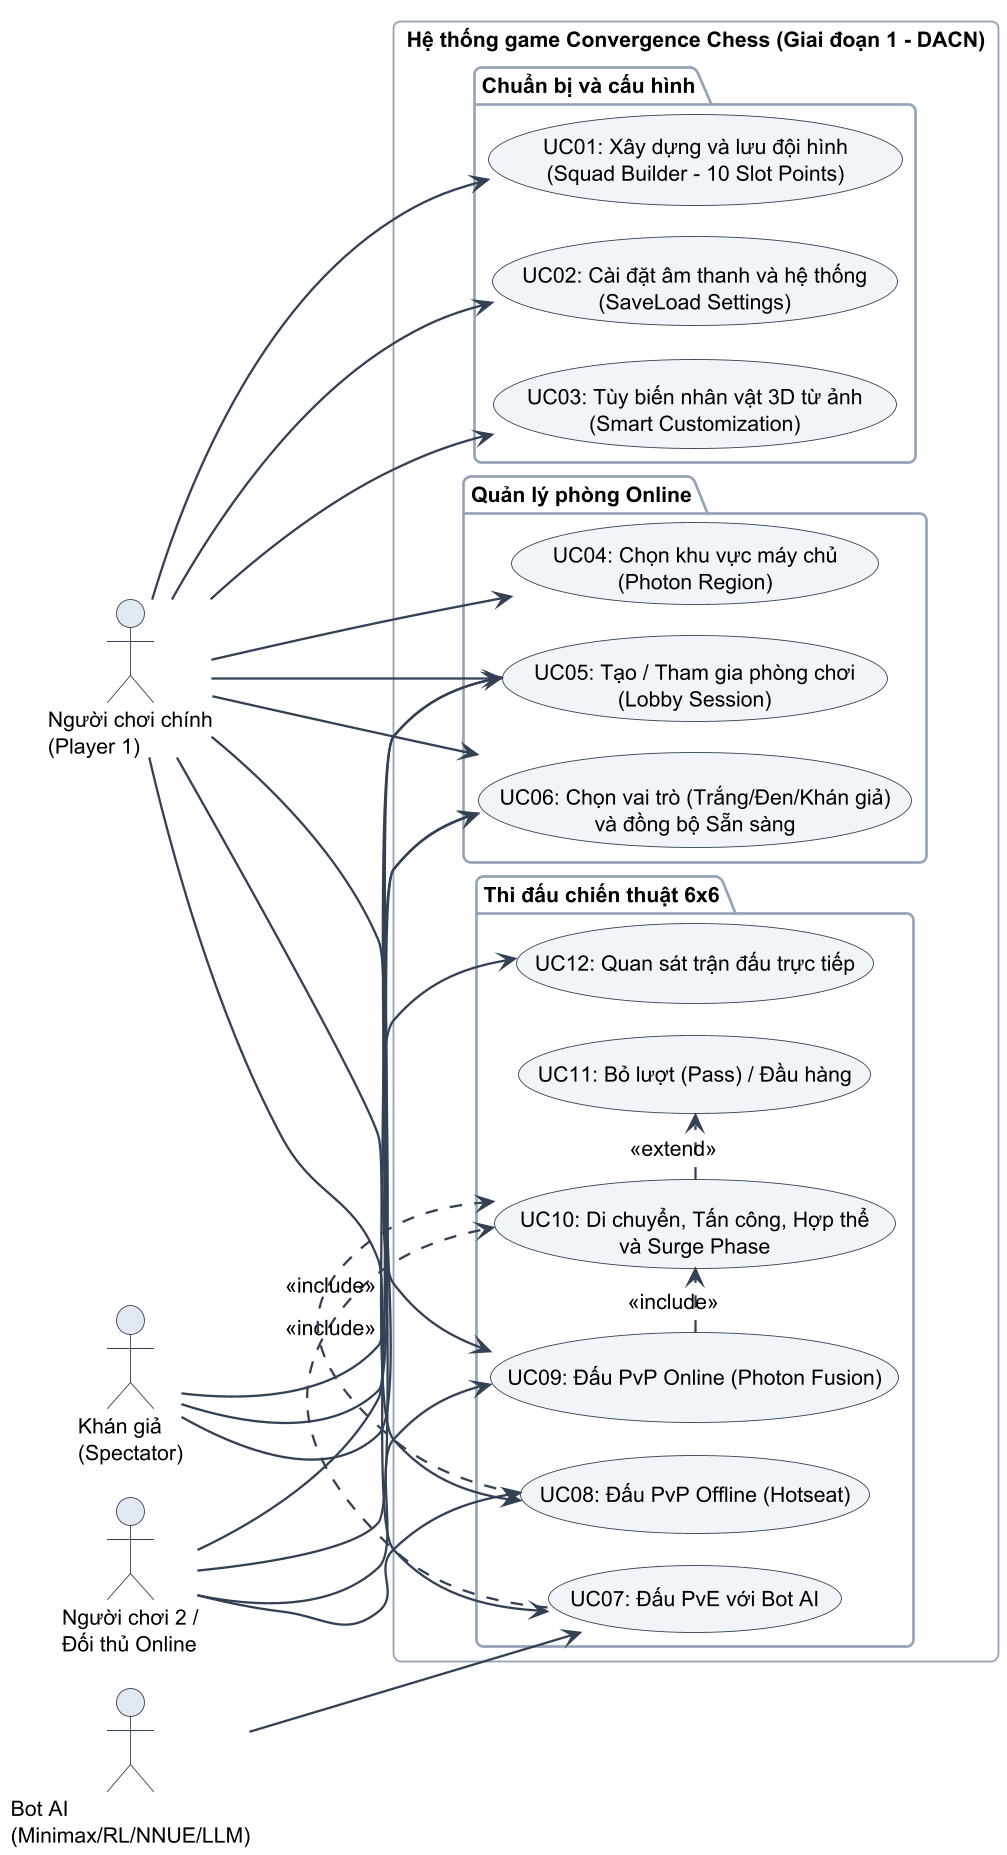
\includegraphics[width=0.72\textwidth,height=0.72\textheight,keepaspectratio]{Diagrams/images/01_usecase_overview.png}
    \caption{Lược đồ Use-case tổng thể hệ thống Convergence Chess}
    \label{fig:usecase_overview}
\end{figure}

{\small
\begin{longtable}{L{2.5cm} L{2.4cm} L{5.3cm} L{4.7cm}}
    \caption{Đặc tả kịch bản cho các Use-case trọng tâm của hệ thống}
    \label{tab:usecase_specs} \\
    \toprule
    \textbf{Use-case} & \textbf{Tác nhân và tiền điều kiện} & \textbf{Luồng sự kiện chính} & \textbf{Luồng ngoại lệ và ràng buộc} \\
    \midrule
    \endfirsthead
    \toprule
    \textbf{Use-case} & \textbf{Tác nhân và tiền điều kiện} & \textbf{Luồng sự kiện chính} & \textbf{Luồng ngoại lệ và ràng buộc} \\
    \midrule
    \endhead
    \bottomrule
    \endfoot
        UC01: Xây dựng và lưu đội hình (Squad Builder) & Người chơi chính; đang ở màn hình Main Menu. & (1) Mở \texttt{UIPopupSquadBuilder}; (2) Kéo thả quân cờ vào 12 ô sân nhà (trừ ô Vua cố định tại chỉ số 3); (3) Hệ thống tính tổng Slot Points thời gian thực theo \texttt{GameplayConfig.MaxSlotsInSquad} (hiện hành $12$ Slot Points) qua \texttt{SquadValidator}; (4) Nhấn Lưu để ghi ra \texttt{SquadSLO} qua \texttt{SaveLoadManager}. & Nếu tổng Slot Points vượt quá hạn mức cấu hình ($12$), chọn quân bị khóa (\texttt{Queen}) hoặc ô đã có quân/Vua, thao tác đặt quân bị chặn và hiển thị thông báo. \\
        \midrule
        UC05--UC06: Tạo/Vào phòng Online, phân vai và Sẵn sàng & Người chơi chính, Đối thủ Online, Khán giả; có kết nối Internet. & (1) Chọn Photon Region và nhập Room ID tại \texttt{UIPopupLobby}; (2) Host mở phòng ở chế độ \texttt{GameMode.Shared} và chiếm vị trí Trắng; (3) Client tham gia, gửi tên người chơi (\texttt{MSG\_MAP\_PLAYER\_NAME}) và yêu cầu đồng bộ slot (\texttt{MSG\_REQUEST\_SLOT\_SYNC}); (4) Chọn vị trí Trắng/Đen/Khán giả, chọn Squad và bật Ready; (5) Khi cả Trắng và Đen sẵn sàng, Host sinh \texttt{MatchSeed} + vật cản và phát \texttt{MSG\_MATCH\_INIT} để đồng loạt tải \texttt{PvPOnlScene}. & Nếu phòng đầy 2 người chơi chính, người vào sau tự động xếp vào danh sách Khán giả (\texttt{Spectator}). Nếu mất kết nối Photon Cloud, hiển thị trạng thái lỗi trên \texttt{OnConnectionStatusChanged}. \\
        \midrule
        UC10--UC11: Thực hiện nước đi, Hợp thể và Surge Phase & Người chơi đang tới lượt hoặc Bot AI; trận đấu đang ở trạng thái \texttt{WaitingInput}. & (1) Chọn quân đồng minh, hệ thống highlight ô hợp lệ; (2) Chọn ô đích để Di chuyển, Tấn công hoặc Hợp thể; (3) \texttt{MoveValidator.ValidateAction} xác thực, \texttt{GameEventHandler.ExecuteCommand} cập nhật \texttt{GameState} và phát \texttt{GameEventBatch}; (4) Nếu vừa Hợp thể và còn đủ AP, mở \texttt{Surge Sub-phase} cho phép đánh bồi hoặc kết thúc lượt giữ AP; (5) Chuyển lượt. & Không đủ AP, chọn ô vật cản với quân trượt, hợp thể 2 quân cùng loại hoặc hợp thể quân đã có \texttt{HasMerged = true} đều bị từ chối. Bỏ lượt bị chặn khi \texttt{PassChargesLeft == 0}; nếu không còn nước đi hợp lệ nào, phe tới lượt bị xử thua. \\
        \midrule
        UC03: Tùy biến nhân vật 3D từ ảnh chân dung (SC) & Người chơi chính; môi trường Python cục bộ chứa \texttt{infer\_onnx.py} và trọng số ONNX/HRN sẵn sàng. & (1) Mở giao diện \texttt{SCCanvasUI}, chọn giới tính (Nam/Nữ), chế độ texture (\texttt{TexNet}/\texttt{HRN}) và ảnh chân dung 2D; (2) \texttt{SCCharacterCreator} khởi chạy tiến trình con \texttt{infer\_onnx.py} qua \texttt{ProcessStartInfo}; (3) Đọc \texttt{sc\_result.json}, ảnh da khử bóng và Normal Map trên ổ đĩa; (4) Tự động áp 25 BlendShapes, màu mắt, màu tóc và cho phép tinh chỉnh thanh trượt hoặc đổi 7 kiểu tóc 3D. & Nếu ảnh không phát hiện khuôn mặt qua MediaPipe hoặc tiến trình Python trả mã lỗi, Unity giữ nguyên nhân vật cơ sở và hiển thị thông báo lỗi mà không treo ứng dụng. \\
\end{longtable}
}

\subsection{Lược đồ kiến trúc tổng thể (Hexagonal Architecture -- Ports \& Adapters)}
Hình \ref{fig:arch_hexagonal} minh họa kiến trúc lục giác (Ports \& Adapters) \cite{cockburn} là xương sống của toàn bộ dự án. Toàn bộ thực thể và quy tắc thẩm định nằm trong khối \textbf{Core Domain} tách khỏi đồ họa, được điều phối vòng lặp bởi \texttt{MatchManager}. Mọi nguồn điều khiển (chuột người chơi, Photon Fusion mạng, các họ Bot AI) đều giao tiếp qua cổng \texttt{IMoveInputProvider}, còn mọi thành phần tiêu thụ kết quả (diễn hoạt 3D, xoay bàn PvP Offline, ghi nhận trận benchmark qua \texttt{BenchmarkGameEventManager}, định hình thưởng \texttt{AgentRewardHandler} hoặc \texttt{NullGameEventListener} cho huấn luyện Headless) đều đi qua cổng \texttt{IGameEventListener} dưới sự điều phối cục bộ của \texttt{ArenaServiceLocator}.

\begin{figure}[H]
    \centering
    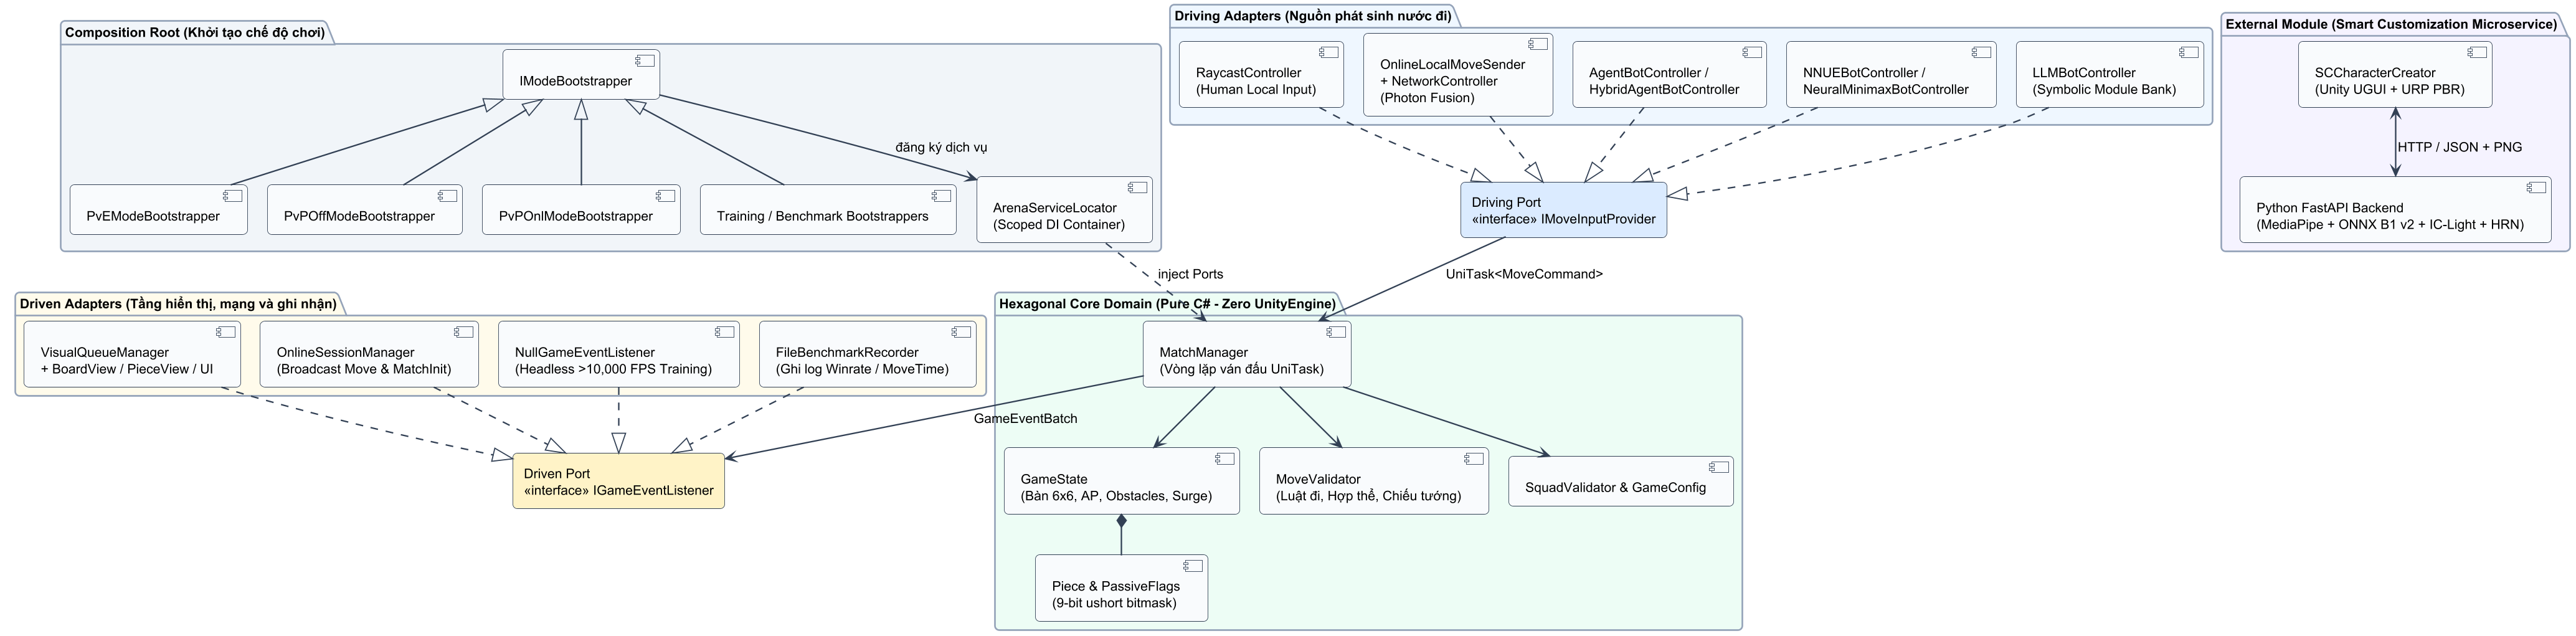
\includegraphics[width=\textwidth]{Diagrams/images/02_architecture_hexagonal.png}
    \caption{Sơ đồ kiến trúc tổng thể theo mô hình Ports \& Adapters và ArenaServiceLocator}
    \label{fig:arch_hexagonal}
\end{figure}

\subsection{Lược đồ lớp (Class diagrams) theo từng phân hệ}
Để bảo đảm khả năng đọc rõ ràng trên khổ giấy A4, lược đồ lớp toàn hệ thống được phân tách thành ba phân hệ chính khớp trực tiếp với cấu trúc thư mục mã nguồn trong \texttt{Assets/Scripts/}.

\subsubsection{Lược đồ lớp phân hệ Core Logic và các bộ điều khiển AI}
Hình \ref{fig:class_core_ai} thể hiện quan hệ giữa \texttt{MatchManager}, \texttt{GameEventHandler}, \texttt{GameState}, \texttt{Piece}, \texttt{MoveValidator} và các lớp thực thi \texttt{IMoveInputProvider} phục vụ AI (\texttt{AgentBotController}, \texttt{NeuralMinimaxBotController}, \texttt{HybridAgentBotController}, \texttt{NNUEBotController}, \texttt{LLMBotController}) kết nối tới \texttt{ObservationEncoderV2}, \texttt{MinimaxSearch}, \texttt{NNUEFastEvaluator}/\texttt{NNUEModelWeights} và \texttt{LLMSymbolicEvaluator}.

\begin{figure}[H]
    \centering
    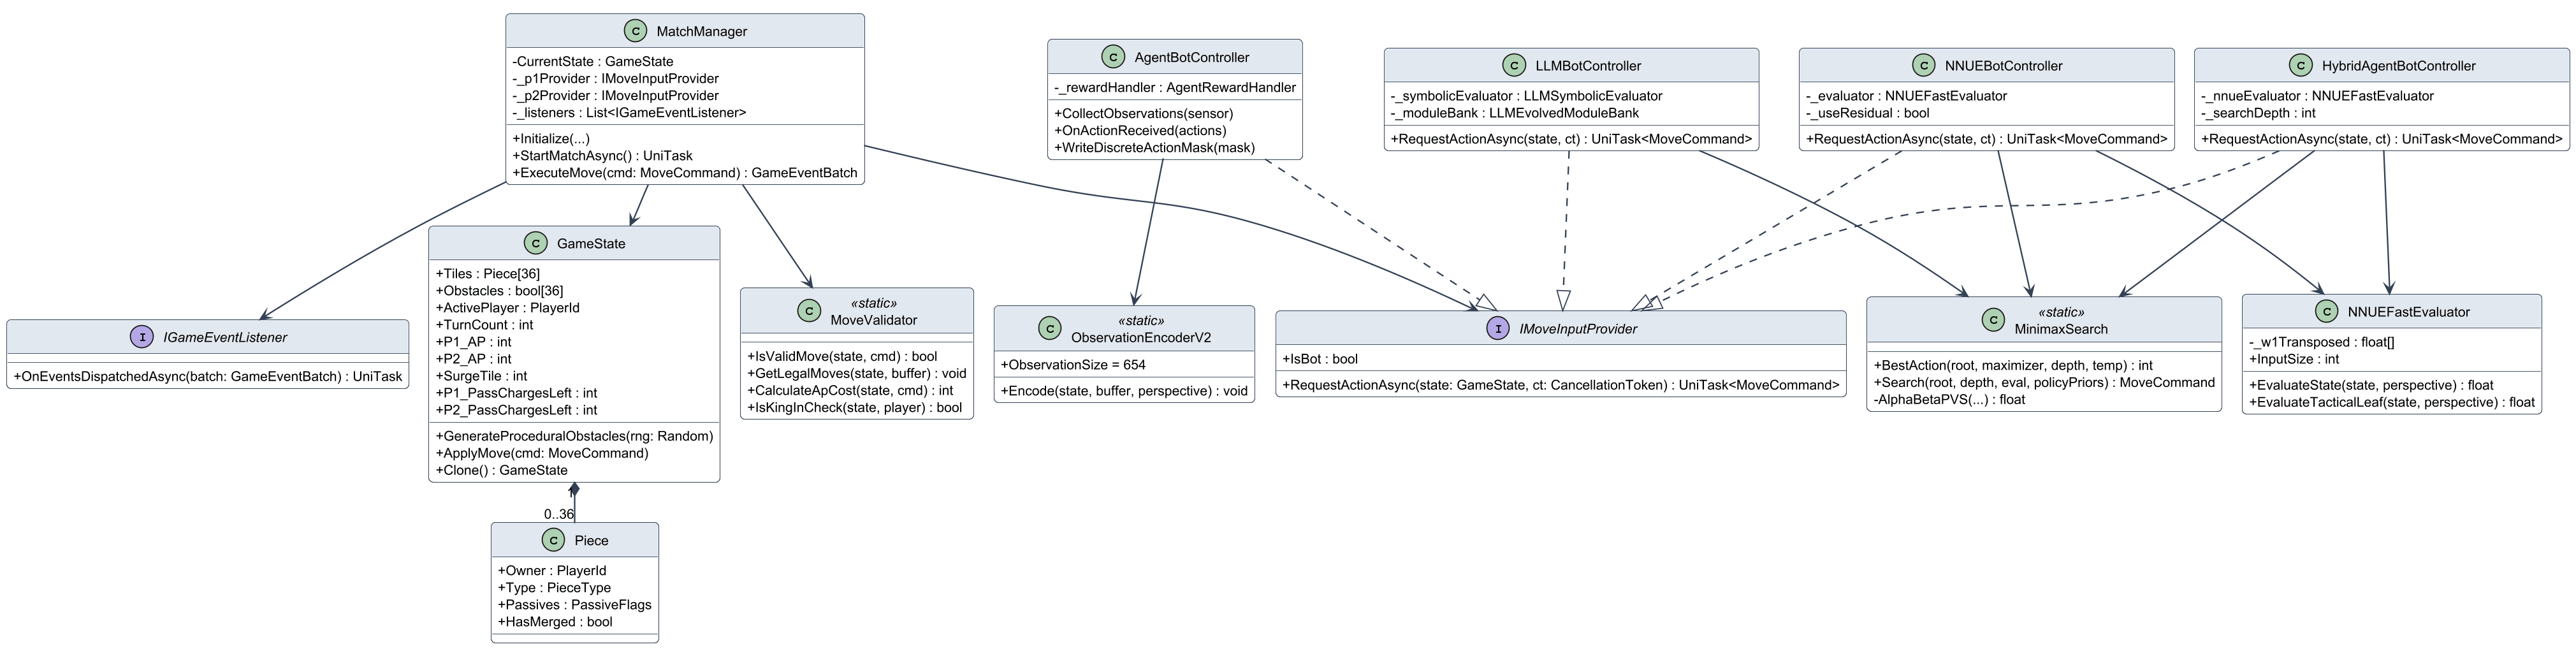
\includegraphics[width=\textwidth]{Diagrams/images/03_class_core_ai.png}
    \caption{Lược đồ lớp phân hệ Core Domain và các tác nhân AI}
    \label{fig:class_core_ai}
\end{figure}

\subsubsection{Lược đồ lớp phân hệ Multiplayer (Photon Fusion)}
Hình \ref{fig:class_network} trình bày kiến trúc mạng tách lớp: \texttt{OnlineSessionManager} điều phối phiên Photon Fusion (\texttt{GameMode.Shared}) và ủy quyền toàn bộ mã hóa/giải mã gói tin nhị phân cho \texttt{OnlineDataBroadcastNetwork}. Lớp định tuyến này sử dụng Factory Method khởi tạo đúng lớp xử lý con kế thừa \texttt{BroadcastDataHandler} dựa trên byte định danh \texttt{BroadcastDataIdentifierByte}. Ở biên giao tiếp với Core, \texttt{NetworkController} (nhận nước đi từ xa qua \texttt{UniTaskCompletionSource}) và \texttt{OnlineLocalMoveSender} (bọc \texttt{RaycastController} để phát nước đi lên mạng) cùng cài đặt \texttt{IMoveInputProvider}.

\begin{figure}[H]
    \centering
    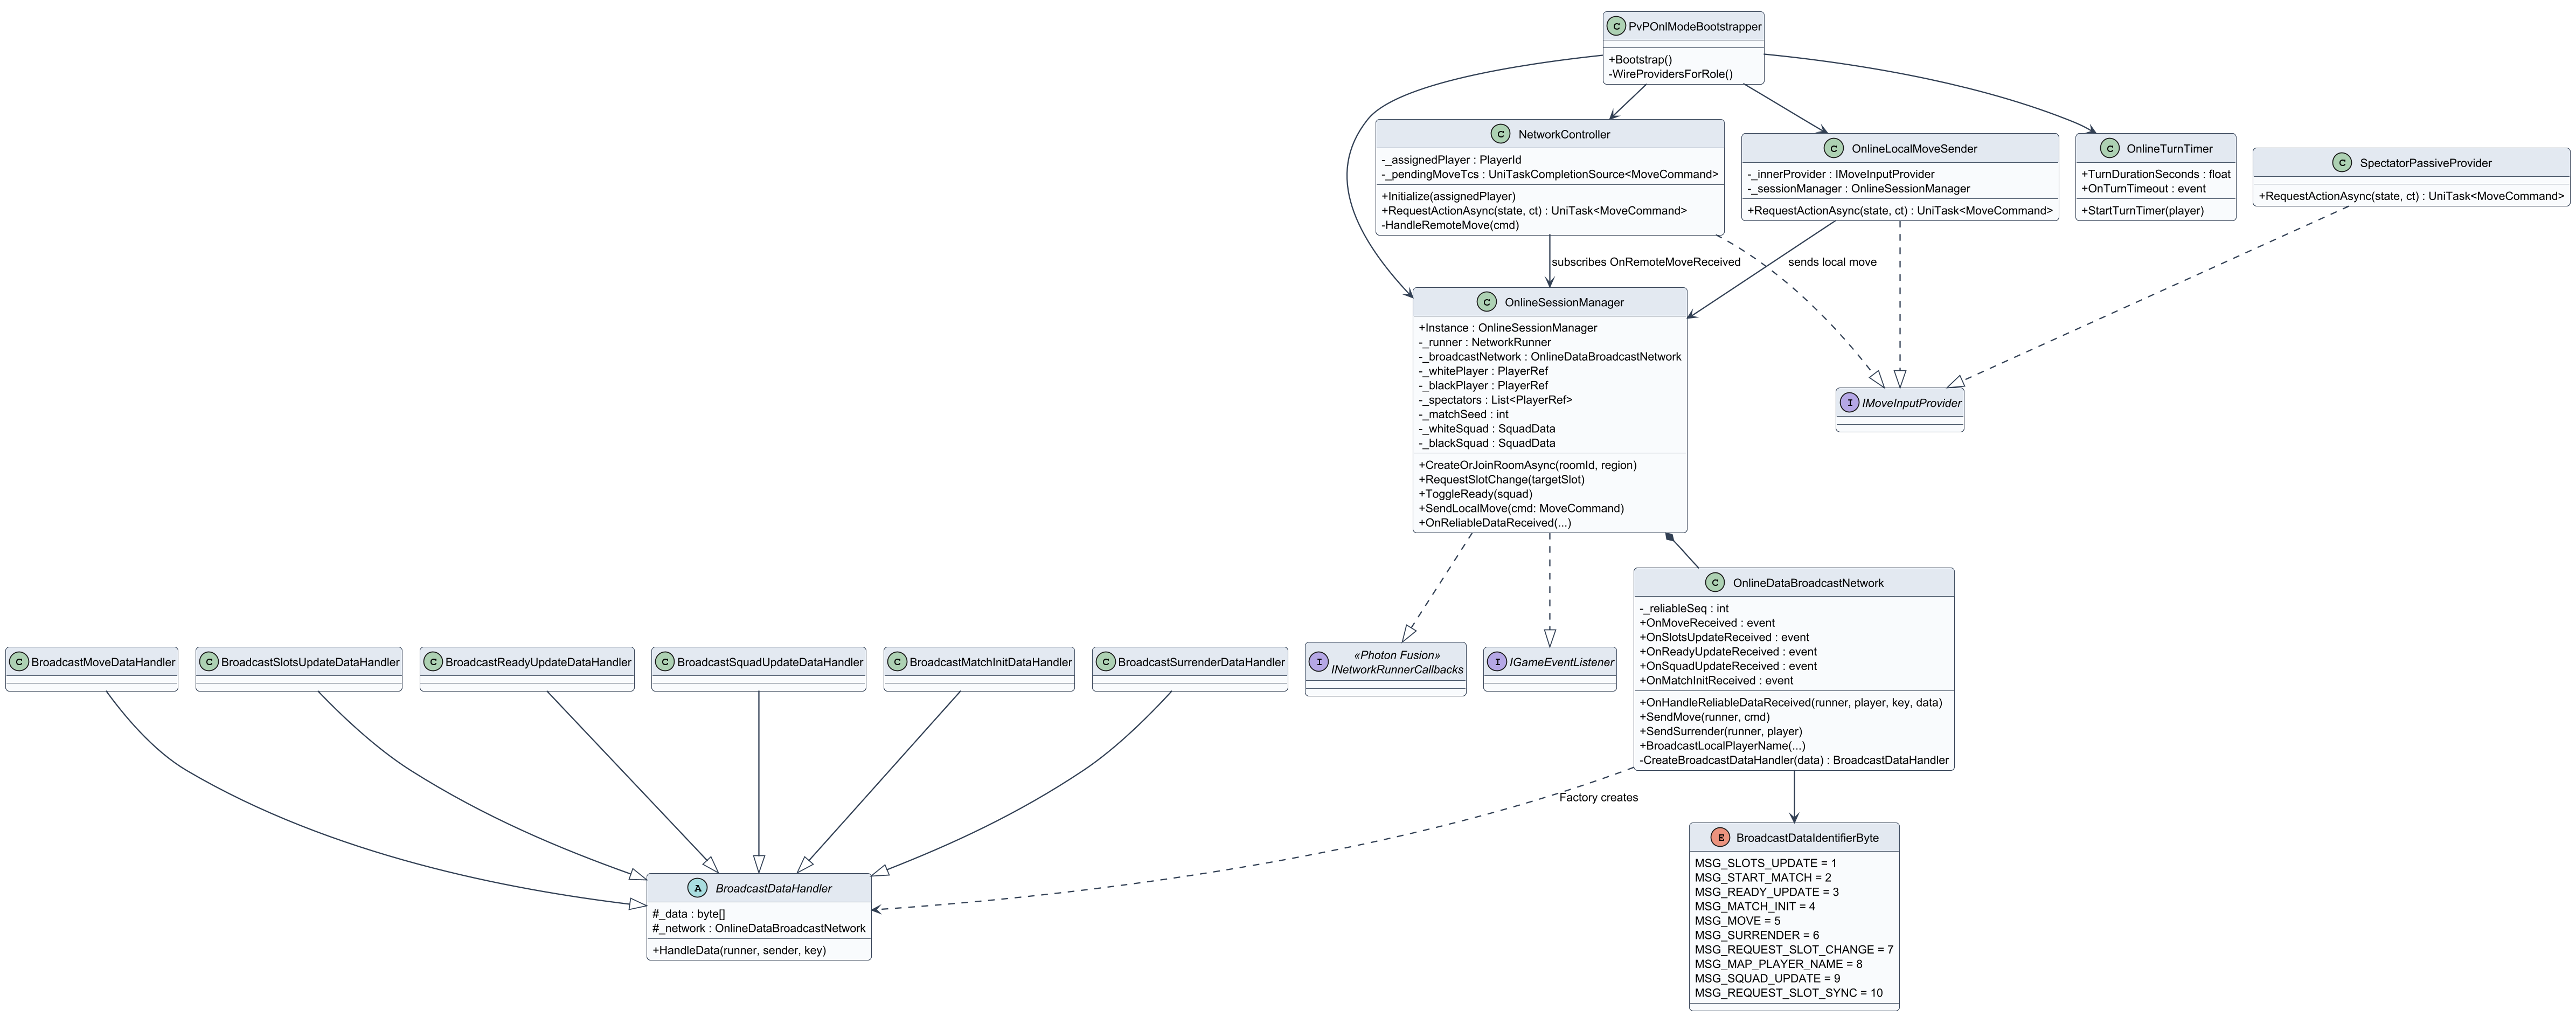
\includegraphics[width=\textwidth]{Diagrams/images/04_class_network.png}
    \caption{Lược đồ lớp phân hệ Multiplayer sử dụng Photon Fusion Reliable Data}
    \label{fig:class_network}
\end{figure}

\subsubsection{Lược đồ lớp phân hệ View Layer và giao diện người dùng (UI)}
Hình \ref{fig:class_view_ui} minh họa luồng trình diễn tách biệt hoàn toàn khỏi Core: \texttt{VisualQueueManager} lắng nghe \texttt{GameEventBatch}, sử dụng \texttt{VisualSequenceBuilder} theo phong cách chuỗi lệnh (\texttt{Then}/\texttt{PlayAsync}) để điều phối các nút diễn hoạt \texttt{IVisualNode} (\texttt{PieceMoveNode}, \texttt{PieceAttackVisualNode}...) tác động lên \texttt{BoardView}, \texttt{TileView} và \texttt{PieceView}. Sự kiện khung hình từ Animator được gom về một đầu mối duy nhất \texttt{PieceAnimationRelay}. Hệ thống giao diện sử dụng \texttt{UIManager} tra cứu prefab tập trung thông qua ScriptableObject \texttt{UIMapper} (Single Source of Truth).

\begin{figure}[H]
    \centering
    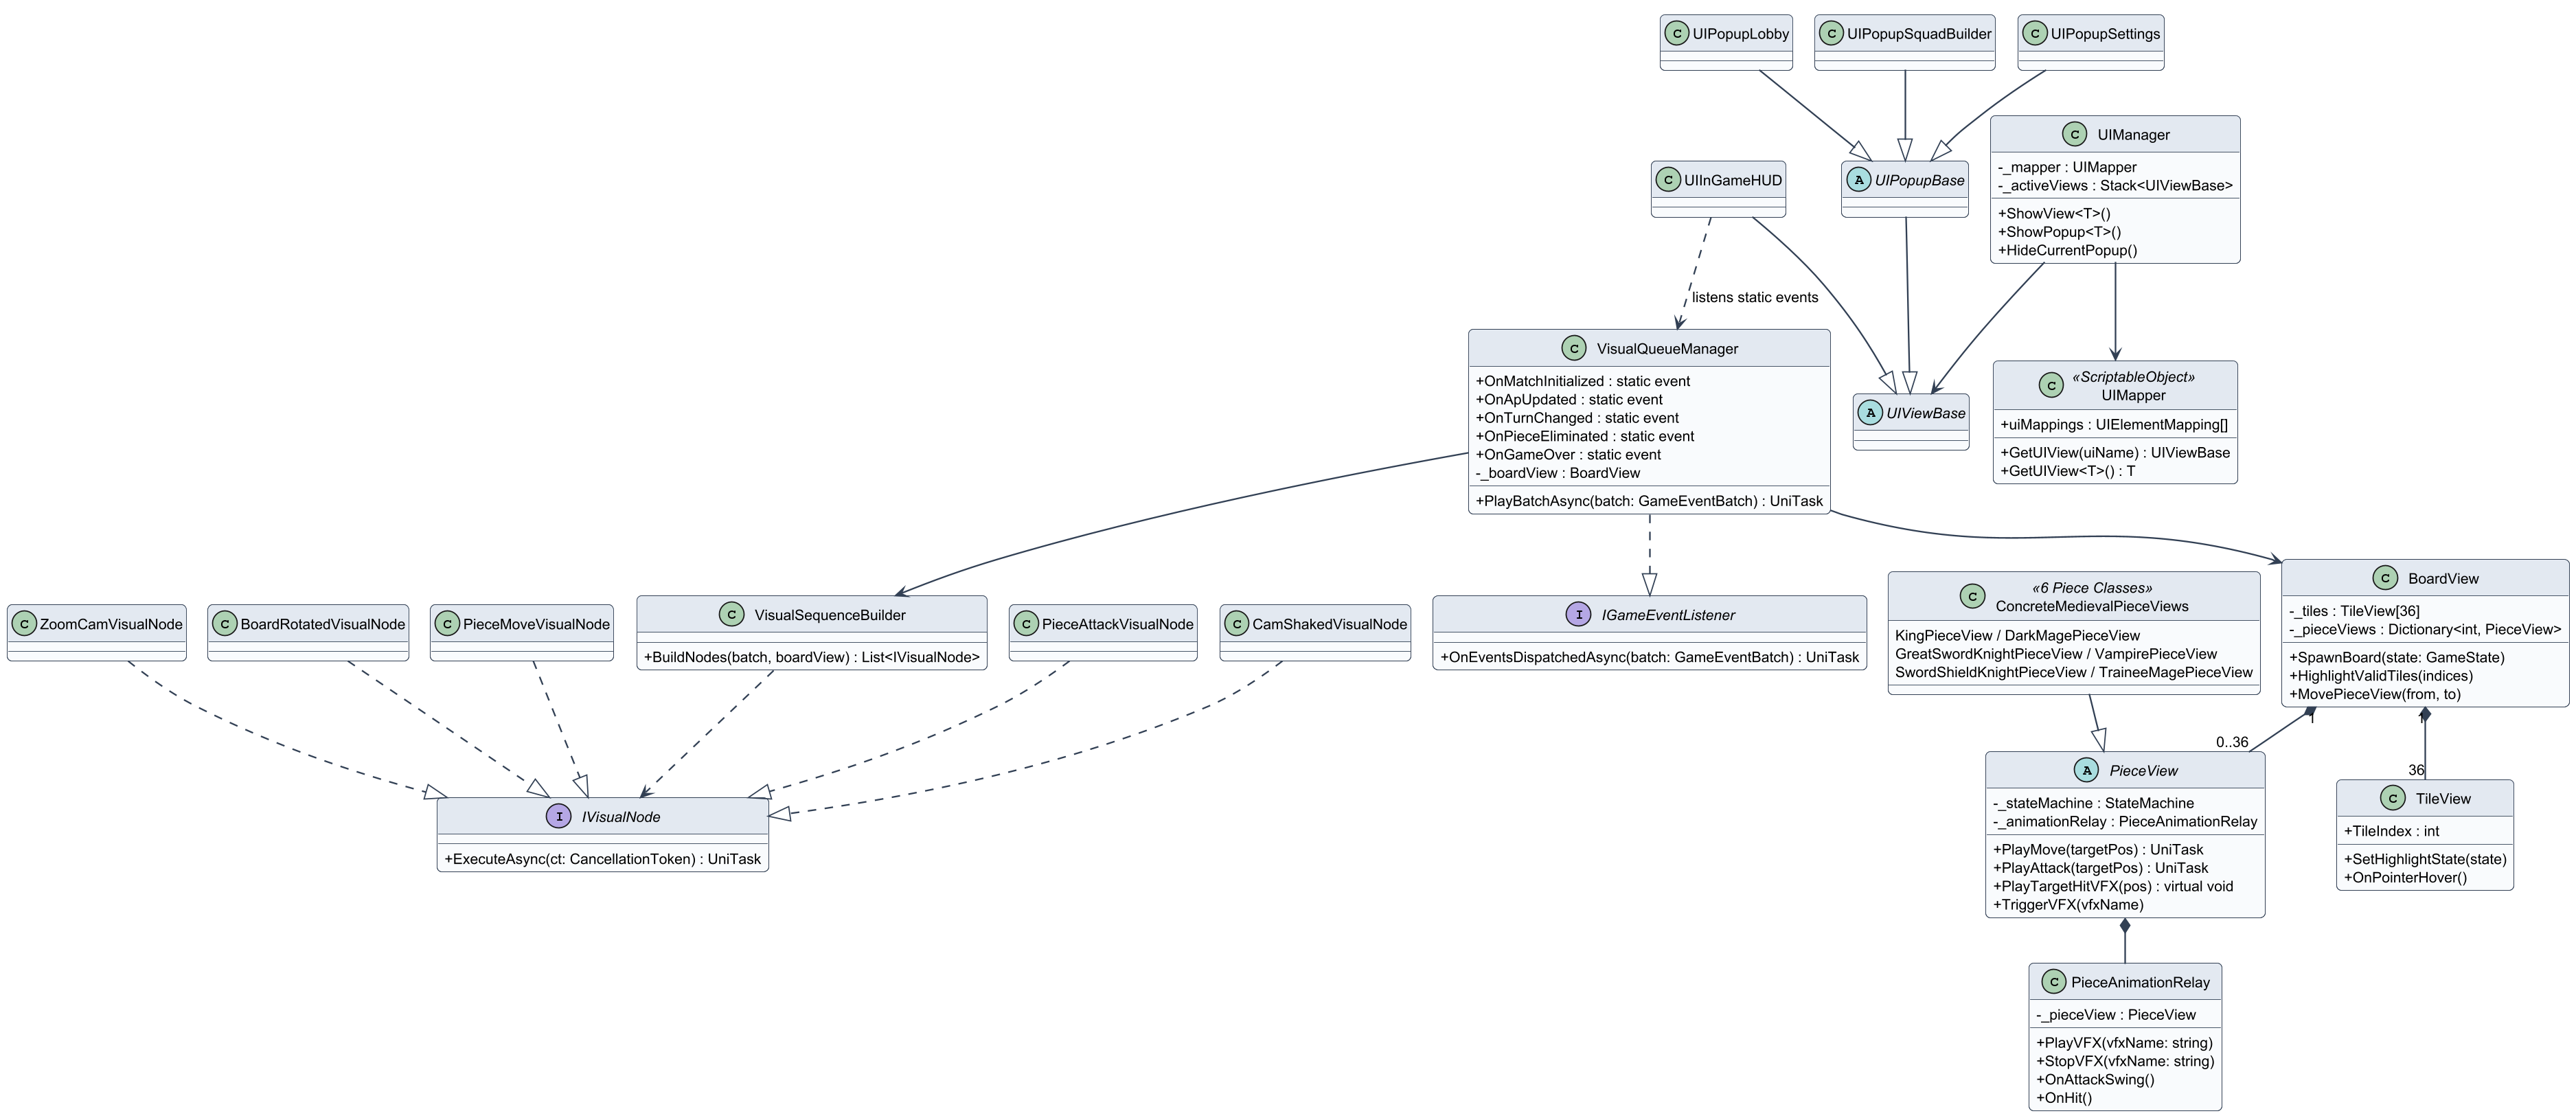
\includegraphics[width=\textwidth]{Diagrams/images/05_class_view_ui.png}
    \caption{Lược đồ lớp phân hệ View Layer, VisualQueueManager và UIManager/UIMapper}
    \label{fig:class_view_ui}
\end{figure}

\subsection{Lược đồ tuần tự (Sequence diagrams) cho luồng Multiplayer Online}
\subsubsection{Luồng khởi tạo phòng, phân vai, đồng bộ đội hình và bắt đầu trận}
Hình \ref{fig:seq_lobby} chi tiết hóa toàn bộ giao thức trao đổi gói tin tin cậy giữa máy Host (Shared Mode Master Client), Photon Fusion Cloud và máy Client từ lúc mở phòng cho tới khi hai máy đồng bộ tuyệt đối cùng một hạt giống bản đồ (\texttt{MatchSeed}), danh sách vật cản trung tuyến và đội hình hai bên.

\begin{figure}[H]
    \centering
    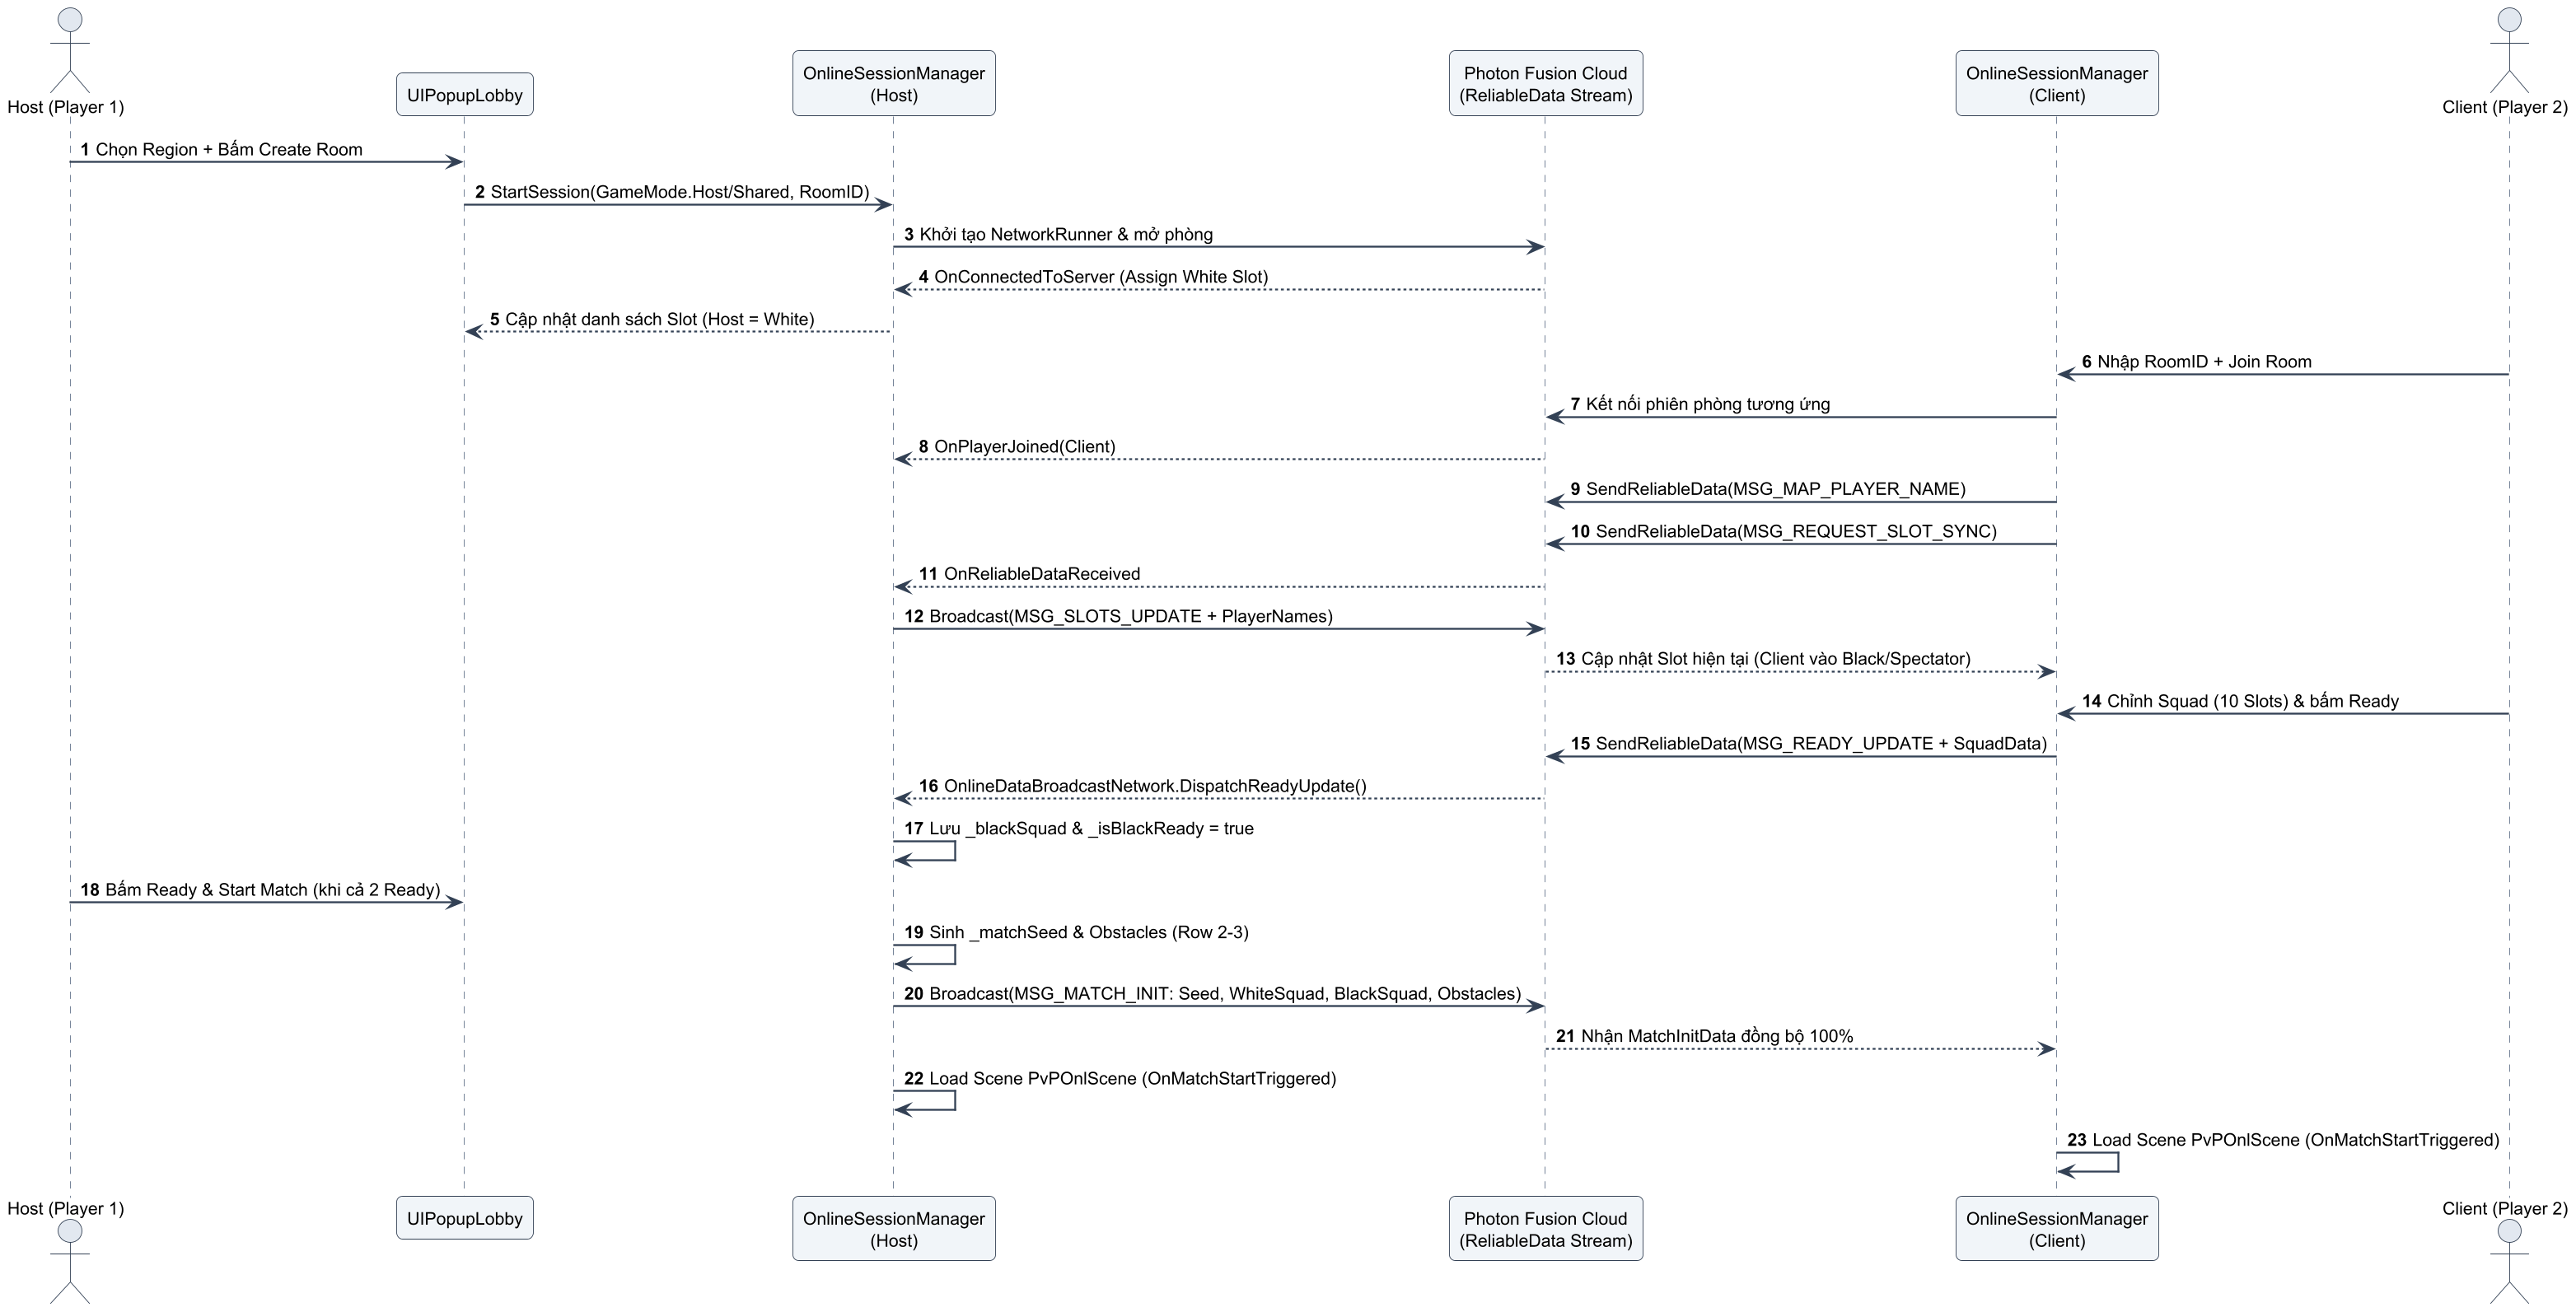
\includegraphics[width=\textwidth]{Diagrams/images/06_seq_pvp_online_lobby.png}
    \caption{Lược đồ tuần tự luồng Lobby, phân vai, đồng bộ đội hình và khởi tạo trận đấu PvP Online}
    \label{fig:seq_lobby}
\end{figure}

\subsubsection{Luồng truyền và thực thi một nước đi hợp lệ trong PvP Online}
Hình \ref{fig:seq_move} mô tả cơ chế đồng bộ nước đi khép kín chỉ với \textbf{4 bytes payload nhị phân} (\texttt{[MSG\_MOVE, FromTile, ToTile, PlayerId]}). Nhờ lõi \texttt{GameState} và \texttt{GameEventHandler} mang tính tất định (Deterministic), khi nước đi hợp lệ được xác nhận cục bộ và phát tới đối thủ qua Photon Reliable Data, cả hai máy đều tự cập nhật trạng thái ván đấu và diễn hoạt độc lập qua \texttt{VisualQueueManager} mà không cần truyền vị trí 3D liên tục từng khung hình.

\begin{figure}[H]
    \centering
    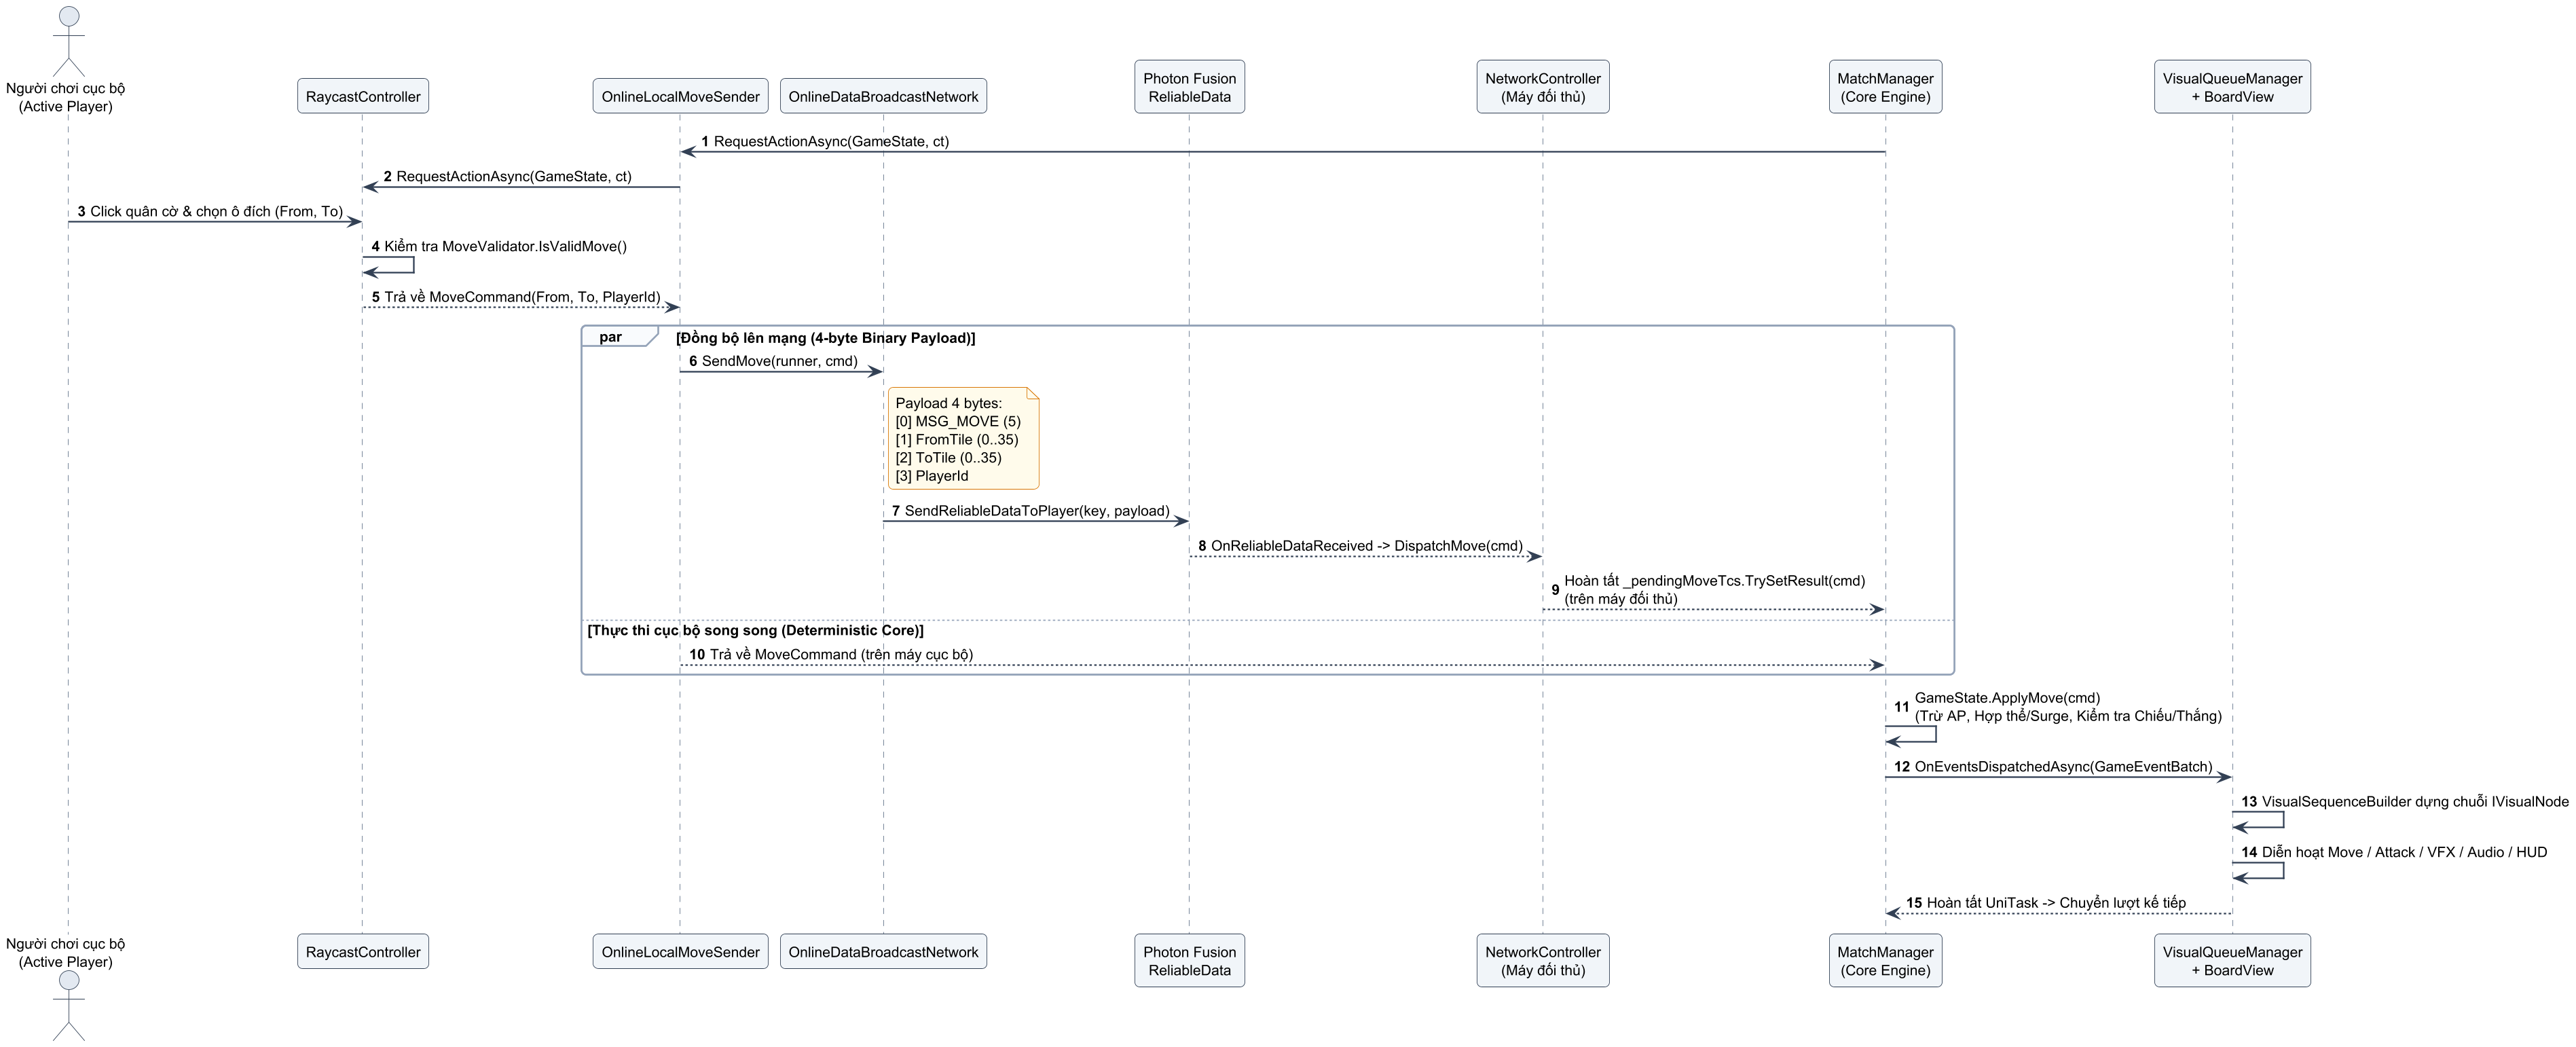
\includegraphics[width=\textwidth]{Diagrams/images/07_seq_pvp_online_move.png}
    \caption{Lược đồ tuần tự luồng gửi, nhận và diễn hoạt một nước đi trong chế độ PvP Online}
    \label{fig:seq_move}
\end{figure}

\subsection{Lược đồ trạng thái (State diagrams) của ván đấu và quân cờ 3D}
Hình \ref{fig:state_machine} tổng hợp hai máy trạng thái quan trọng nhất: (i) vòng đời một trận đấu trong \texttt{MatchManager}/\texttt{GameEventHandler}/\texttt{GameState} thể hiện rõ nhánh chuyển sang \texttt{SurgeSubPhase} sau khi hợp thể cùng đầy đủ các điều kiện kết thúc trận; và (ii) máy trạng thái 5 pha của \texttt{PieceView} (\texttt{IdleStateBase}, \texttt{MoveStateBase}, \texttt{AttackStateBase}, \texttt{GetHitStateBase}, \texttt{DeathStateBase} cùng các lớp con theo từng quân cờ).

\begin{figure}[H]
    \centering
    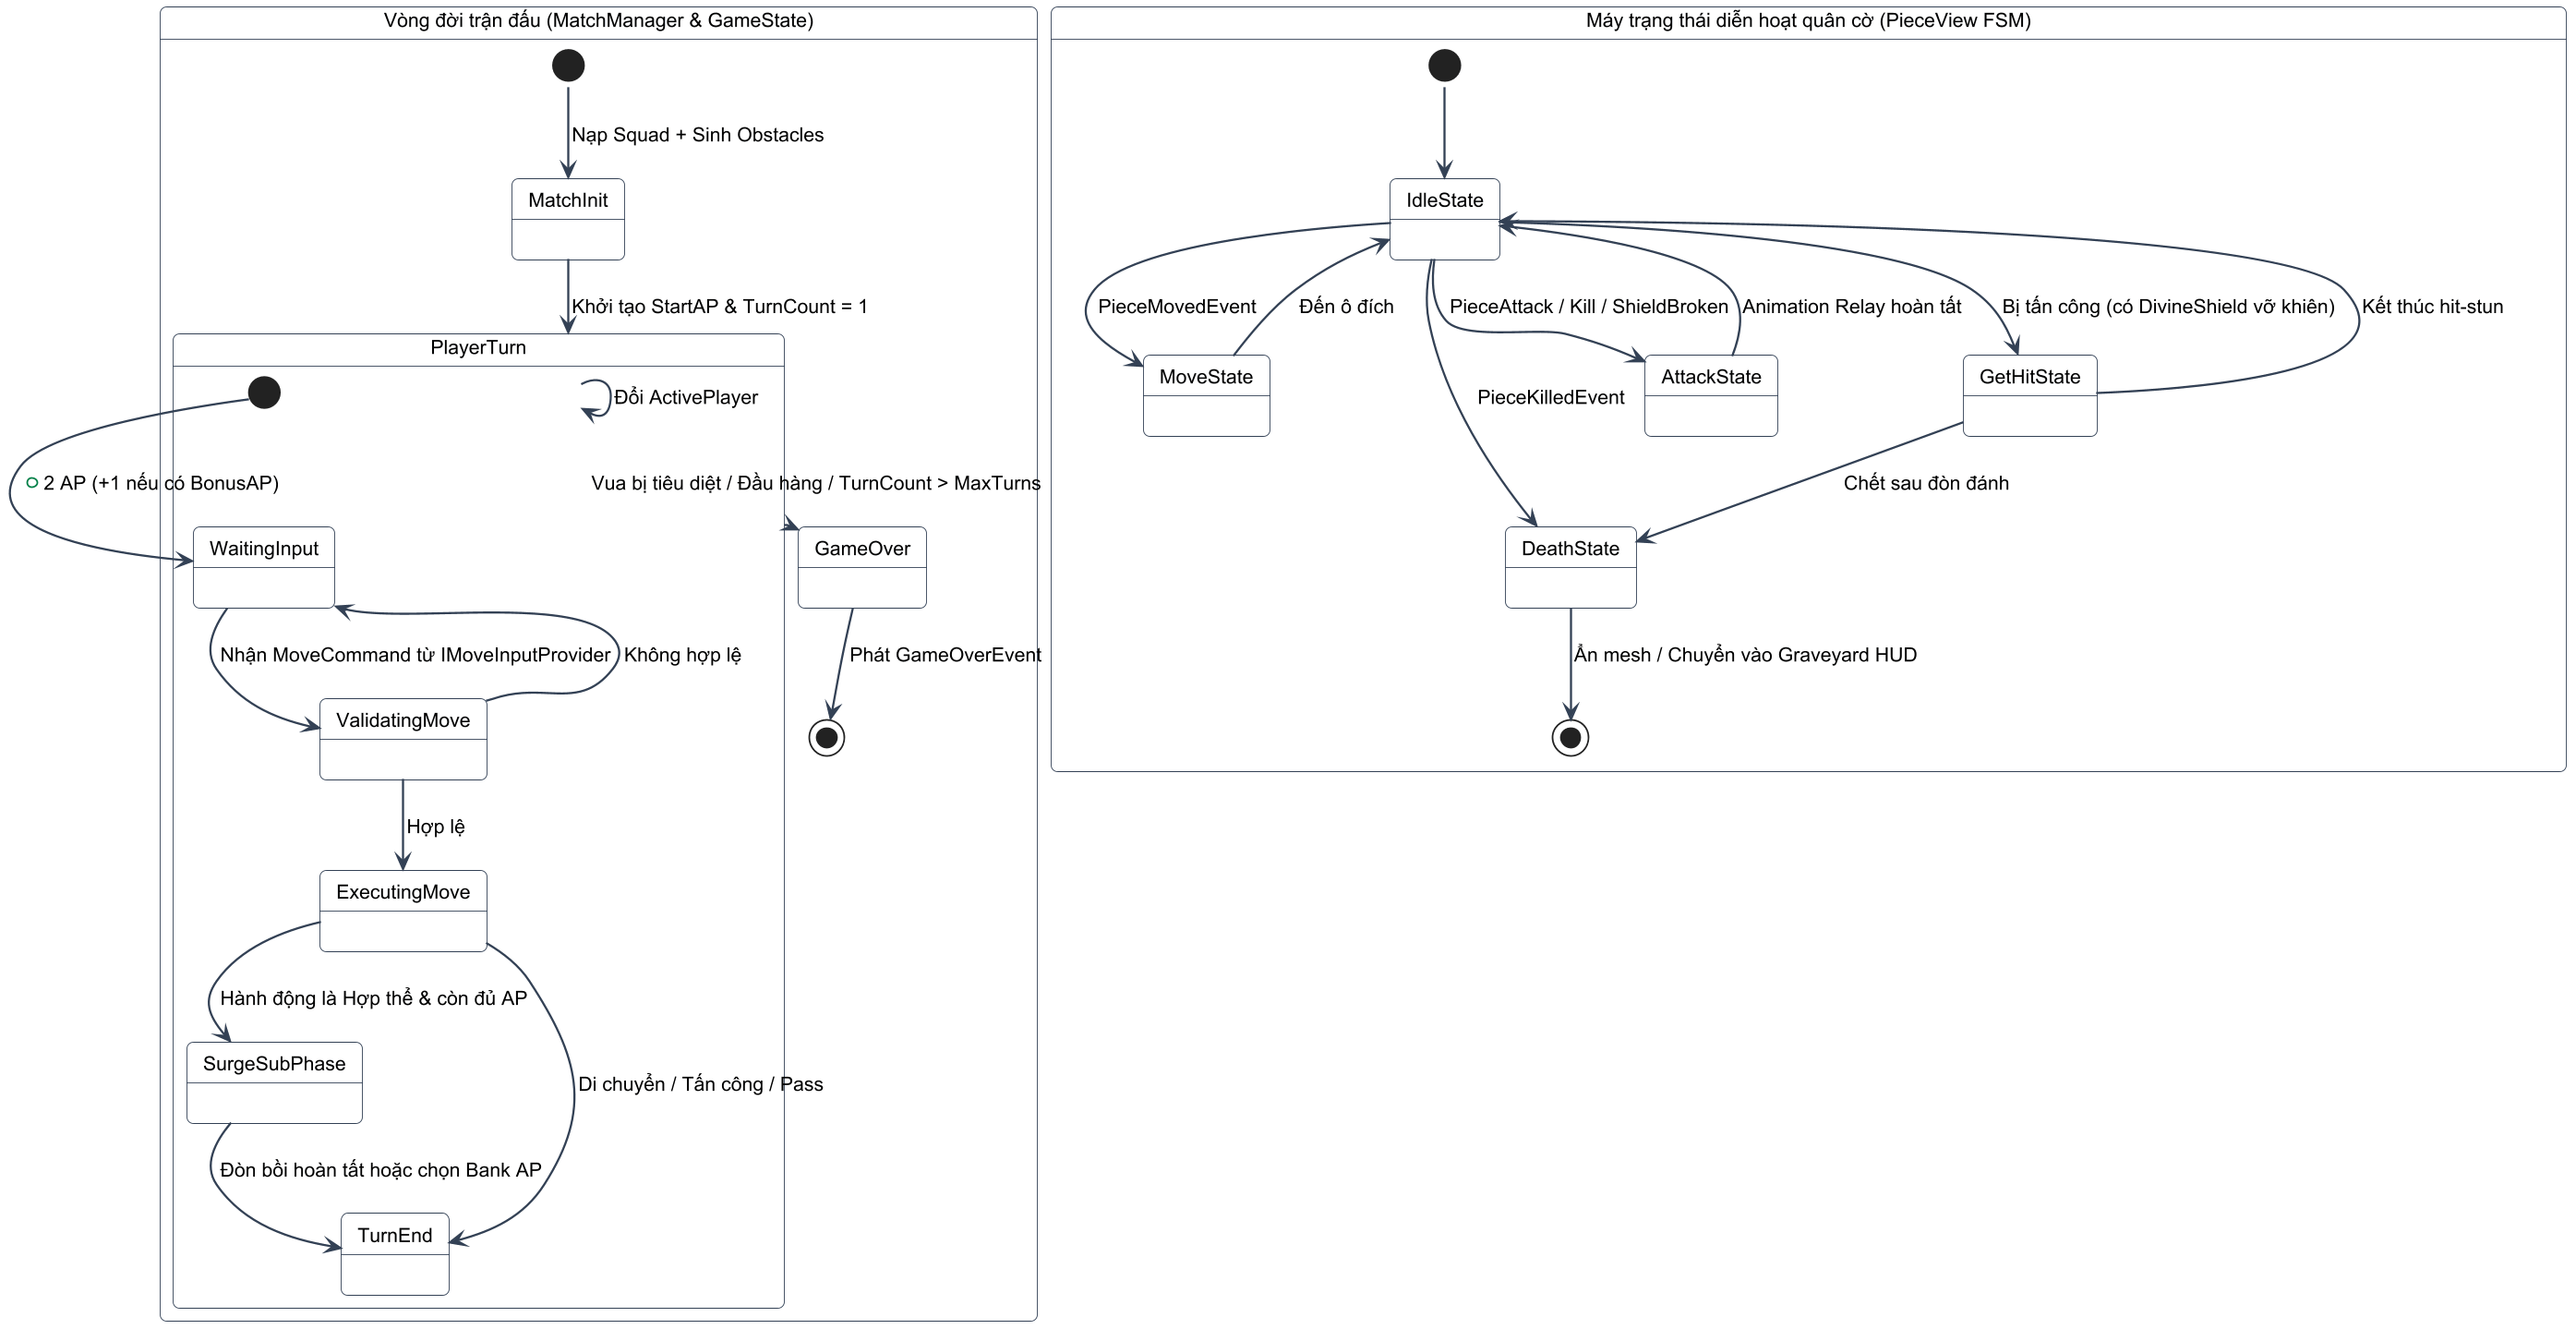
\includegraphics[width=0.96\textwidth]{Diagrams/images/08_state_piece_and_match.png}
    \caption{Lược đồ trạng thái vòng đời trận đấu (MatchManager) và diễn hoạt quân cờ (PieceView FSM)}
    \label{fig:state_machine}
\end{figure}

\subsection{Sơ đồ quy trình huấn luyện AI đa thế hệ và Smart Customization}
Hình \ref{fig:pipeline_ai} khái quát hóa hệ sinh thái 5 tầng huấn luyện và kiểm chuẩn AI trong dự án, thể hiện vòng lặp đồng huấn luyện (Iterative Co-training) giữa ML-Agents PPO và mạng giá trị NNUE/Residual NNUE cùng nhánh tiến hóa luật biểu tượng bằng LLM.

\begin{figure}[H]
    \centering
    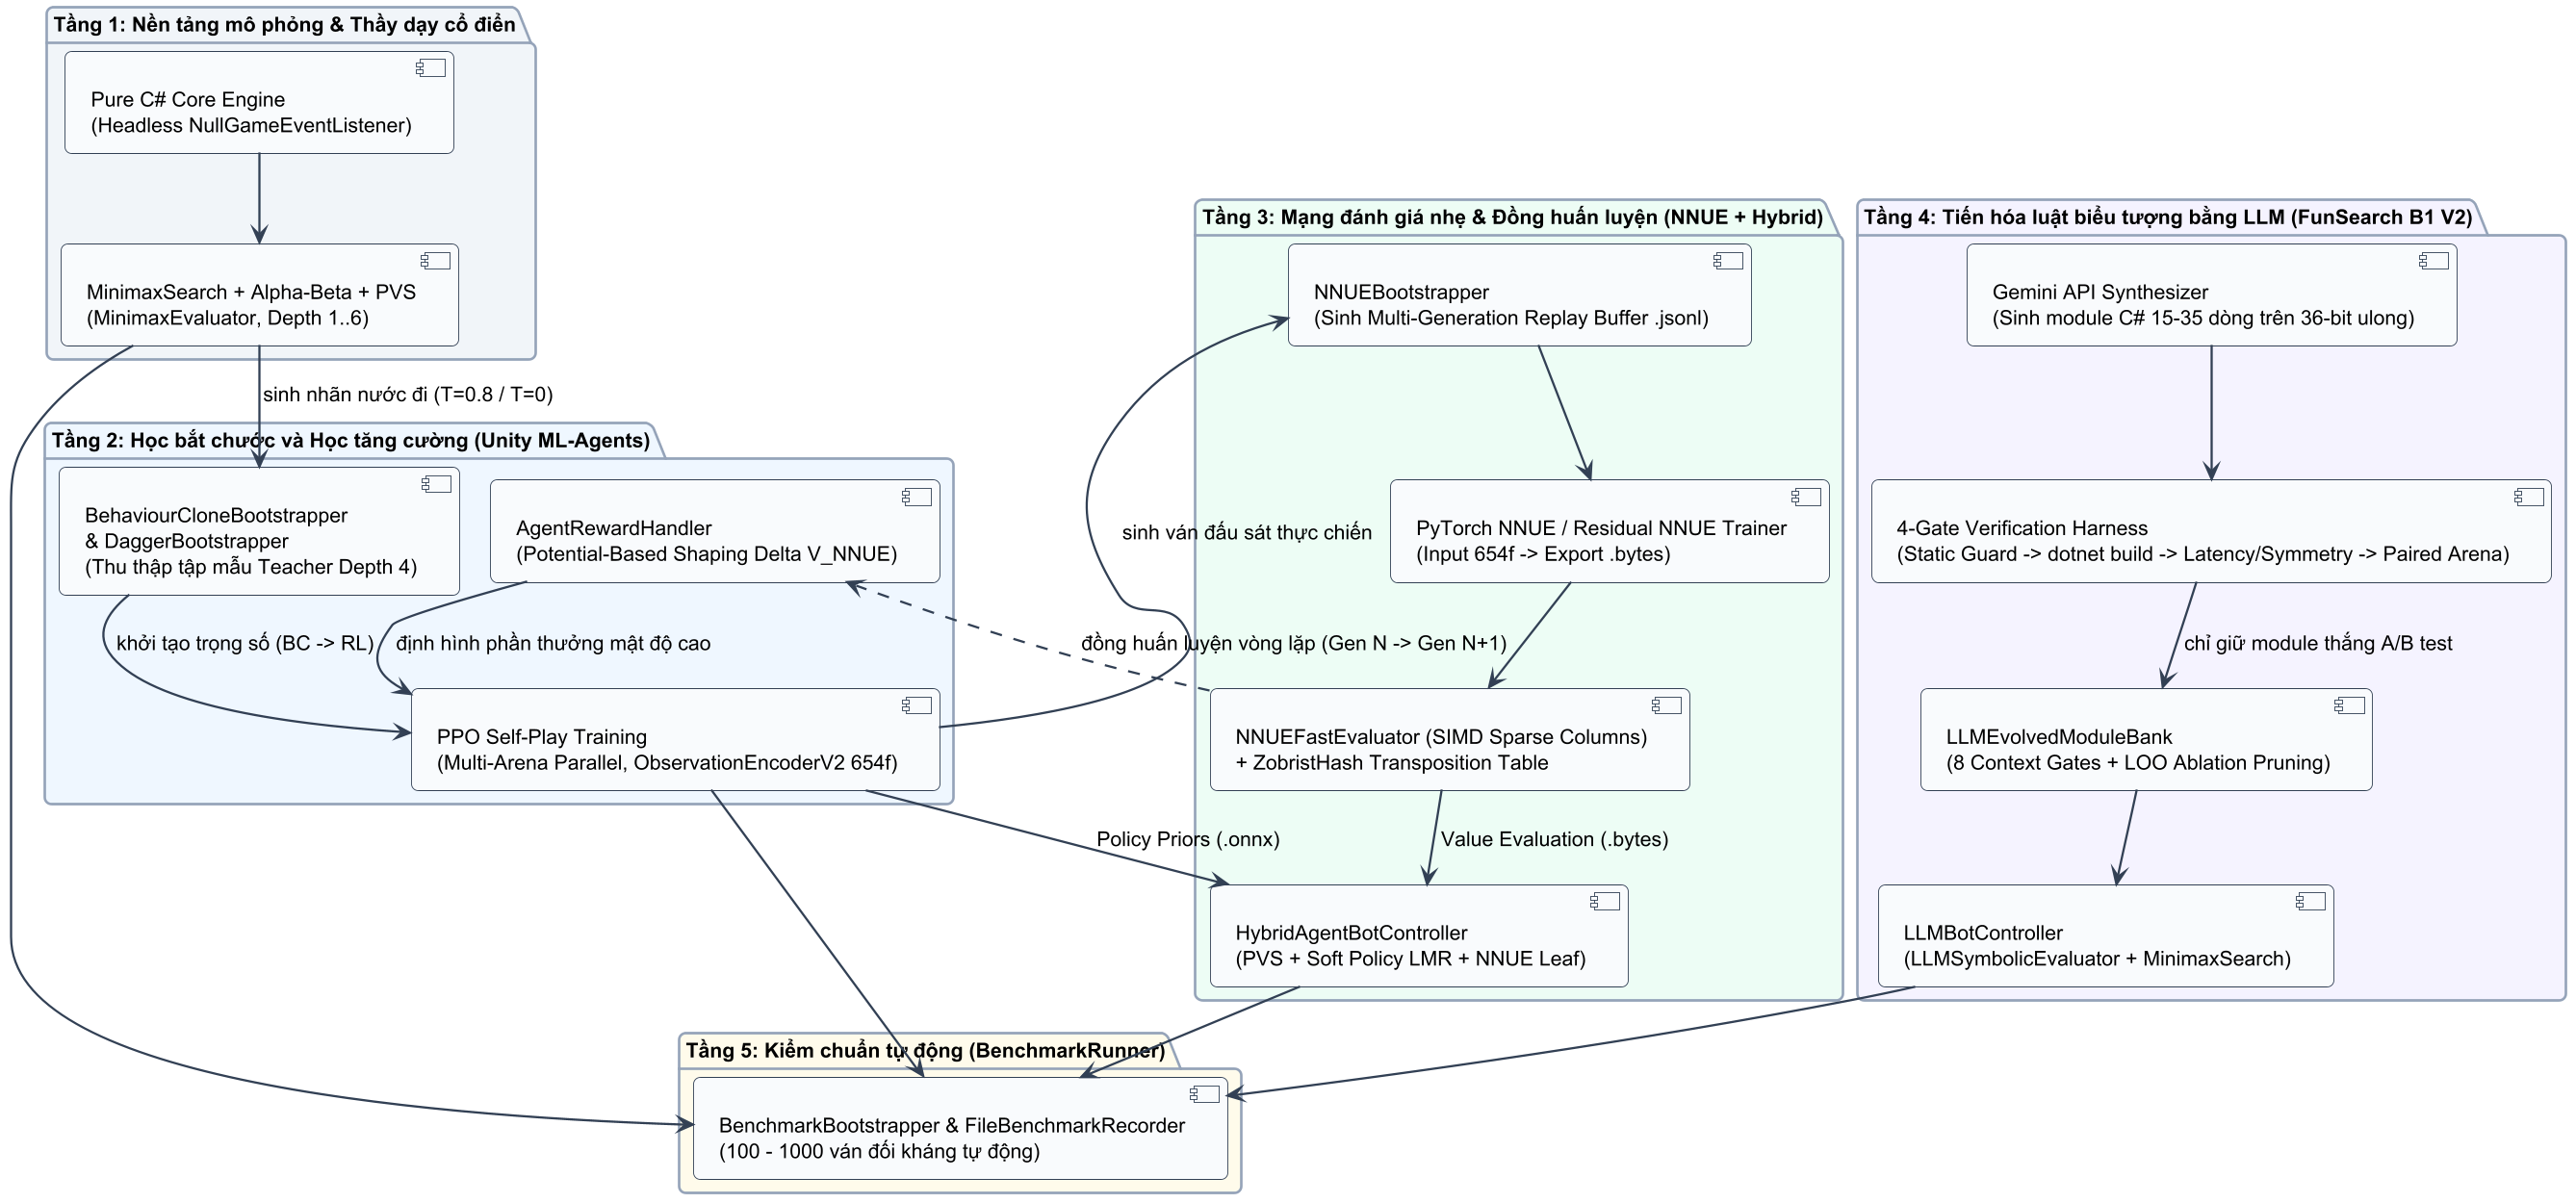
\includegraphics[width=0.96\textwidth]{Diagrams/images/09_pipeline_ai_training.png}
    \caption{Sơ đồ quy trình huấn luyện AI đa thế hệ (Minimax, BC/DAgger, PPO, NNUE, Hybrid và LLM)}
    \label{fig:pipeline_ai}
\end{figure}

Hình \ref{fig:pipeline_sc} trình bày kiến trúc tích hợp cục bộ giữa Unity 6 URP Client (\texttt{SCCharacterCreator}) và tiến trình Python \texttt{infer\_onnx.py} (chạy qua CLI subprocess và trao đổi tệp JSON/PNG) xử lý đồng thời hai nhánh Hình học khuôn mặt (Method B1 v2) và Chiếu Texture UV -- Khử bóng đối xứng (PyTorch3D Barycentric + Bilateral Symmetry Delighting + Multi-Band Pyramid + HRN).

\begin{figure}[H]
    \centering
    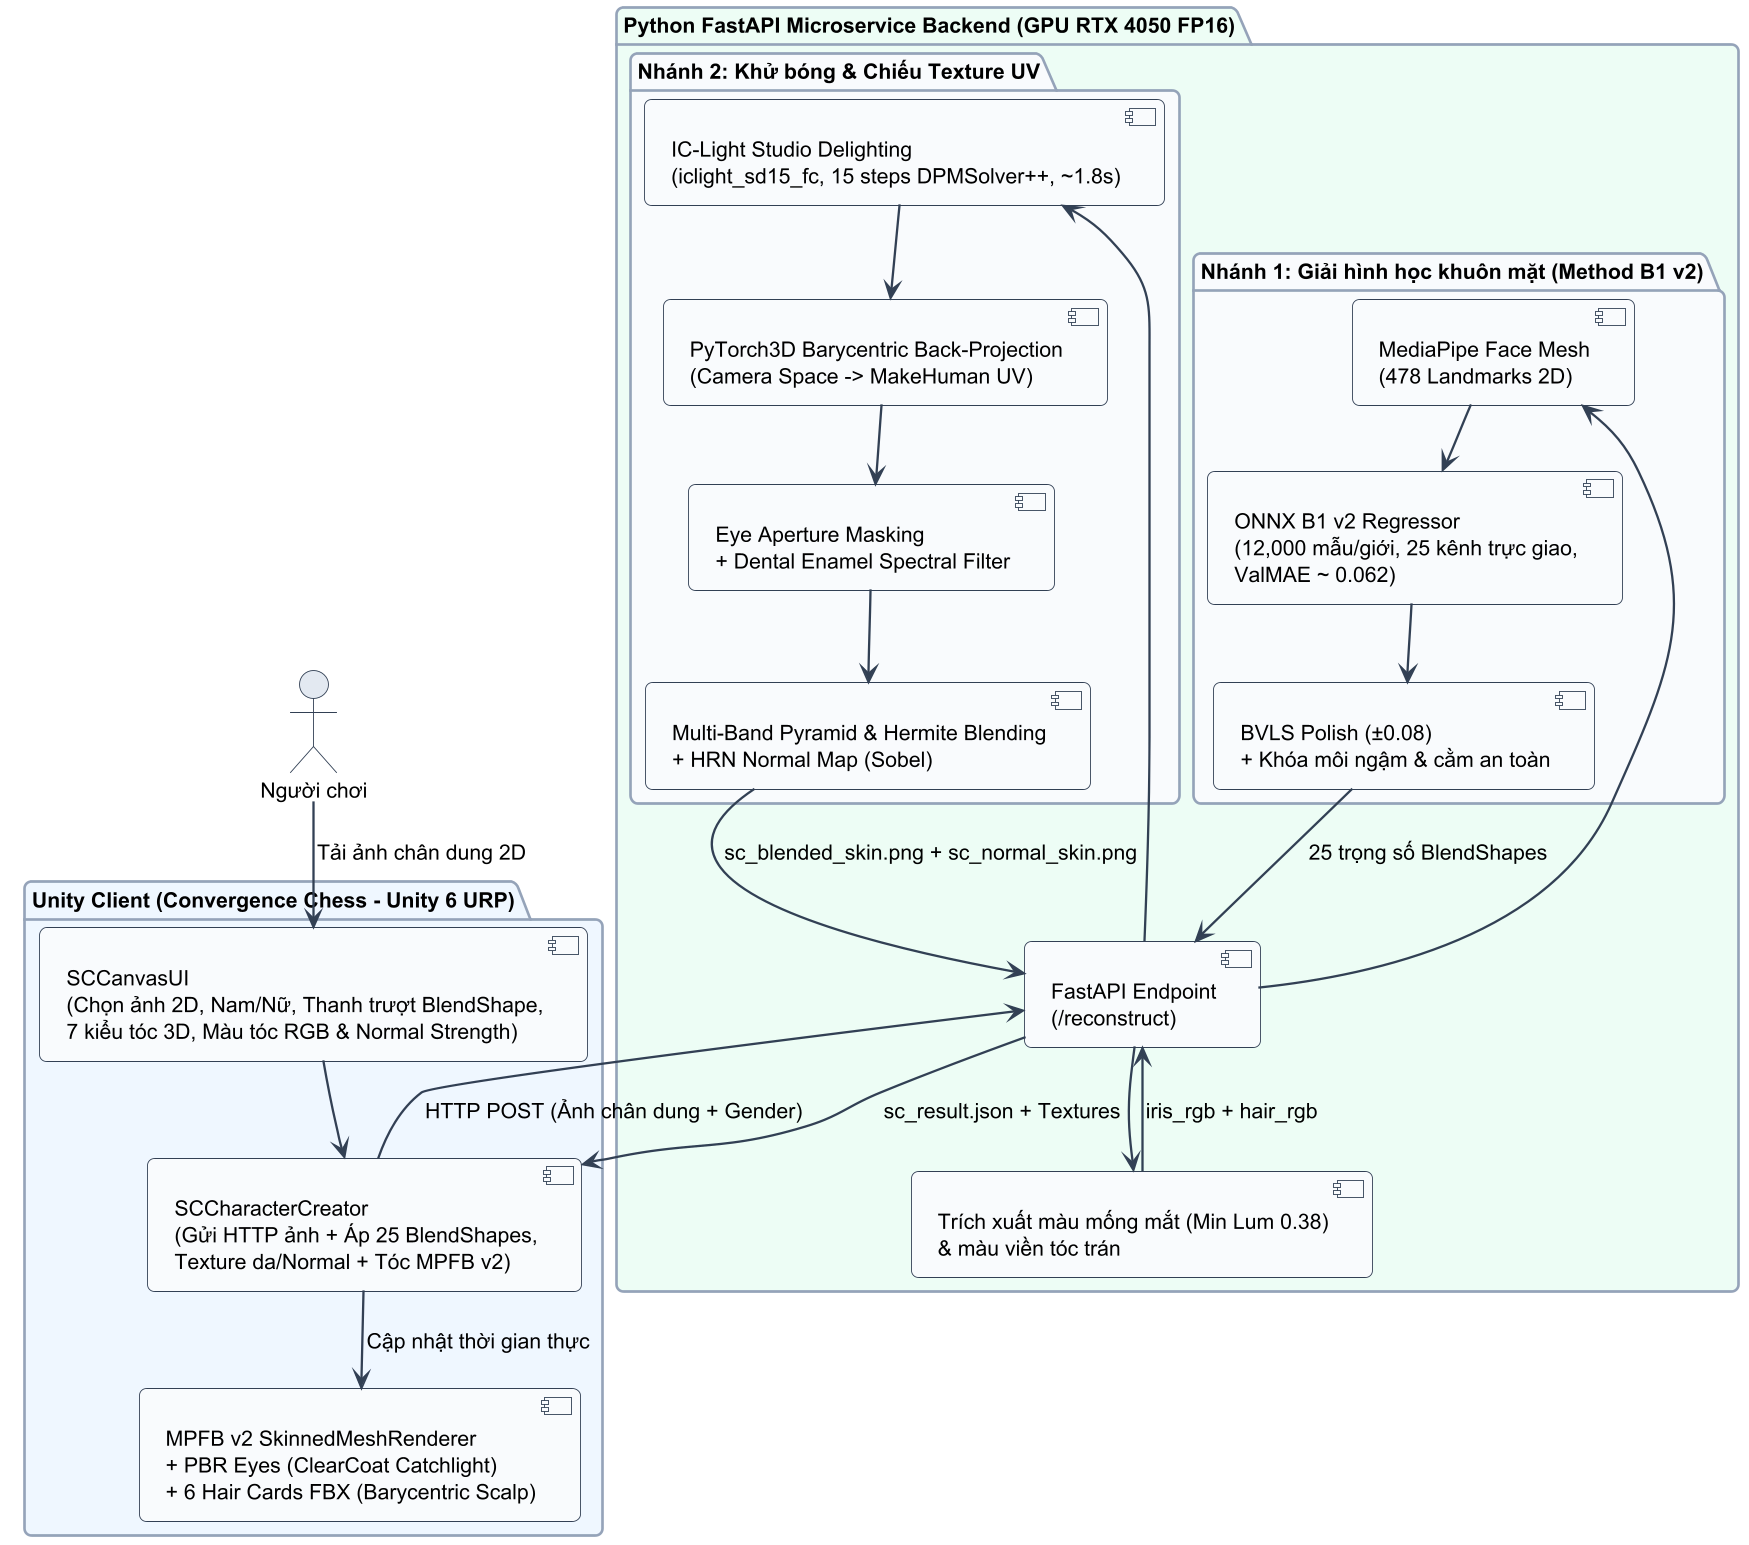
\includegraphics[width=0.88\textwidth]{Diagrams/images/10_pipeline_smart_customization.png}
    \caption{Sơ đồ kiến trúc xử lý cục bộ cho phân hệ tùy biến nhân vật 3D (Smart Customization)}
    \label{fig:pipeline_sc}
\end{figure}

\newpage

% Chương 5: Phân tích thiết kế và hiện thực hệ thống (gồm 3 phân hệ lớn)
\section{Thiết kế và hiện thực hệ thống}
\subsection{Thiết kế và hiện thực phân hệ lõi luật chơi}

\subsubsection{Tổ chức kiến trúc lõi tách rời và cấu hình cân bằng tập trung}
Từ phân tích đánh đổi giữa các hướng triển khai trên Unity ở Mục 3.2, toàn bộ phần xử lý luật chơi của \textit{Convergence Chess} được thiết kế tách rời hoàn toàn khỏi đồ họa 3D và tổ chức quanh ba khối thành phần chính (minh họa tổ chức đối tượng và tài nguyên cấu hình trong Unity tại Hình \ref{fig:unity_core_config}):
\begin{itemize}
    \item \textbf{Nguồn cấu hình cân bằng tập trung:} Lưu toàn bộ tham số trò chơi (ngân sách $12$ điểm đội hình, chi phí điểm và chi phí AP của từng loại quân, mức hồi $+2$ AP mỗi lượt, trần tích lũy $5$ AP, phụ phí hợp thể hiện đặt bằng $0$, giới hạn $3$ lượt bỏ và $60$ lượt đấu) trong một tài nguyên dữ liệu tĩnh độc lập (\texttt{ScriptableObject} của Unity). Cách tổ chức này giúp nhóm điều chỉnh cân bằng lối chơi nhanh chóng mà không phải sửa trực tiếp logic xử lý.
    \item \textbf{Cấu trúc trạng thái ván đấu thống nhất:} Lưu tập trung toàn bộ dữ liệu của một trận đấu trong cùng một cấu trúc duy nhất, gồm vị trí quân cờ trên lưới $36$ ô, $1$--$2$ vật cản vùng trung tuyến (ô $12$ đến ô $23$) sinh theo hạt giống xác định, tập $9$ kỹ năng nội tại của từng quân cờ (được biểu diễn gọn dưới dạng tập cờ trạng thái giúp thao tác hợp thể và sao chép bàn cờ diễn ra tức thời), điểm hành động hai bên, trạng thái đòn bồi Surge và số lượt còn lại.
    \item \textbf{Cô lập hoàn toàn theo từng bàn đấu:} Thay vì dùng bộ quản lý toàn cục dễ gây xung đột dữ liệu, mỗi bàn đấu sở hữu một vùng quản lý dịch vụ riêng được lắp ráp linh hoạt theo từng chế độ chơi (đấu với máy, đấu hai người cùng máy, đấu trực tuyến hoặc mô phỏng huấn luyện AI). Ở chế độ huấn luyện AI, tầng diễn hoạt đồ họa được tắt hoàn toàn để chạy song song hàng chục bàn cờ cùng lúc.
\end{itemize}

\begin{figure}[H]
    \centering
    \screenshotplaceholder{Content/Core và AI/images/unity\_core\_config\_hierarchy.png}{Chụp ảnh cấu trúc bàn đấu mẫu (Prefab Arena) trong cửa sổ Hierarchy cùng tài nguyên cấu hình cân bằng trò chơi (ScriptableObject) trong Unity Editor.}
    \caption{Tổ chức bàn đấu độc lập và nguồn cấu hình cân bằng tập trung trong Unity 6}
    \label{fig:unity_core_config}
\end{figure}

\subsubsection{Luồng vận hành một lượt đấu và kiểm định luật chơi}
Vòng lặp trận đấu vận hành theo cơ chế bất đồng bộ từng lượt, kết nối với bên ngoài qua hai cổng thống nhất (cổng tiếp nhận hành động và cổng phát sự kiện). Một lượt chơi diễn ra tuần tự qua bốn bước:
\begin{enumerate}
    \item \textbf{Khởi tạo đầu lượt:} Hệ thống cộng điểm hành động đầu lượt ($+2$ AP cơ bản và cộng thêm từ kỹ năng đặc biệt, tối đa $5$ AP) và kiểm tra xem phe tới lượt còn ít nhất một nước đi hoặc quyền bỏ lượt hợp lệ hay không; nếu không còn hành động nào, trận đấu kết thúc và xử thua cho phe đó.
    \item \textbf{Tiếp nhận nước đi theo chế độ chơi:} Hệ thống chờ nhận lệnh hành động (di chuyển, tấn công, hợp thể hoặc bỏ lượt) từ đúng nguồn điều khiển của phe đang tới lượt, bao gồm thao tác chuột của người chơi, dữ liệu từ đối thủ trực tuyến hoặc quyết định từ tác nhân AI.
    \item \textbf{Thẩm định toàn diện tính hợp lệ:} Bộ thẩm định luật chơi kiểm tra đồng thời mọi điều kiện của nước đi:
    \begin{itemize}
        \item Đủ lượng AP cần thiết theo loại quân và khoảng cách di chuyển; đường trượt không bị chặn bởi quân cờ khác hoặc vật cản trung tuyến (ngoại trừ quân có kỹ năng nhảy chữ L).
        \item Tuân thủ đầy đủ quy tắc hợp thể: cấm hợp thể hai quân cùng loại gốc, mỗi quân chỉ tham gia hợp thể tối đa một lần trong trận và không cho phép quân Vua tham gia hợp thể.
        \item Khi đang ở giai đoạn đòn bồi Surge, chỉ cho phép quân cờ vừa hợp thể thực hiện hành động hoặc chọn kết thúc lượt để giữ lại AP.
        \item Kiểm tra trạng thái chiếu Vua, xử lý tương tác giữa Khiên hộ mệnh với Phá khiên và phong cấp Tốt khi tiến tới hàng cuối sân đối phương.
    \end{itemize}
    \item \textbf{Cập nhật trạng thái và phát đợt sự kiện:} Sau khi nước đi hợp lệ được áp dụng lên trạng thái bàn cờ, lõi xử lý gom toàn bộ các hệ quả phát sinh trong nước đi đó (di chuyển, hợp thể, vỡ khiên, tiêu diệt quân, phong cấp Tốt, kích hoạt Surge, tiêu hao AP, đổi lượt hoặc kết thúc trận) thành một đợt sự kiện tuần tự gửi sang tầng hiển thị. Riêng trong quá trình duyệt cây tìm kiếm của AI, lõi luật hỗ trợ đi thử và hoàn tác trực tiếp mà không tạo sự kiện hình ảnh để tối đa hóa tốc độ mô phỏng.
\end{enumerate}

\subsubsection{Đánh giá ưu và nhược điểm của kiến trúc lõi tách rời}
\begin{itemize}
    \item \textbf{Ưu điểm:} Bảo đảm tính nhất quán tuyệt đối giữa mọi chế độ chơi (đấu máy, đấu hai người cùng máy và đấu trực tuyến); đạt tốc độ mô phỏng hàng trăm ván đấu trong vài chục giây cho huấn luyện AI nhờ chạy không đồ họa và biểu diễn trạng thái gọn nhẹ; thuận lợi khi viết kiểm thử tự động cho các tình huống biên của luật chơi.
    \item \textbf{Nhược điểm và đánh đổi:} Chi phí thiết kế ban đầu cao hơn so với cách viết trực tiếp vào đối tượng 3D của Unity; mỗi khi bổ sung một cơ chế luật mới, nhóm phải đồng bộ thêm loại sự kiện tương ứng ở lớp cầu nối sang tầng hiển thị.
\end{itemize}

\subsection{Thiết kế và hiện thực hệ thống trí tuệ nhân tạo}

Đóng góp nghiên cứu trọng tâm của Giai đoạn 1 là xây dựng và kiểm chứng hai dòng tác nhân AI chính là \textbf{Hybrid Bot} và \textbf{LLM Bot}, cùng giao tiếp với lõi trò chơi thông qua một giao diện nhận nước đi thống nhất. Để đánh giá khách quan, báo cáo đối chiếu hai dòng này với hai mốc truyền thống là mạng tự quyết định nước đi (không tìm kiếm) và Minimax thuần ở Chương 6.

\subsubsection{Bộ mã hóa trạng thái bàn cờ}
Toàn bộ hệ thống AI dùng chung một bộ mã hóa trạng thái gồm \textbf{654 đặc trưng số thực} ($36\text{ ô} \times 18\text{ kênh} + 6\text{ biến toàn cục}$), luôn được chuẩn hóa theo góc nhìn của phe đang tới lượt:
\begin{itemize}
    \item Mỗi ô trên bàn cờ $6 \times 6$ được mô tả bằng $18$ kênh thông tin: $1$ kênh đánh dấu ô vật cản, $6$ kênh loại quân cờ có dấu ($+1$ với quân mình, $-1$ với quân địch cho 6 loại quân từ Tốt đến Vua), $9$ kênh tương ứng với $9$ kỹ năng nội tại có dấu theo phe sở hữu, $1$ kênh trạng thái đã từng hợp thể và $1$ kênh đánh dấu ô đang kích hoạt Surge.
    \item Sáu biến toàn cục biểu diễn lượng AP hiện có của hai bên, số lượt bỏ lượt còn lại của hai bên, tiến độ trận đấu so với giới hạn $60$ lượt và cờ báo hiệu đang ở giai đoạn Surge.
\end{itemize}
Không gian hành động rời rạc gồm $36 \times 36 + 1 = 1{,}297$ lựa chọn (ánh xạ mọi cặp ô xuất phát -- ô đích và hành động cuối cùng là bỏ lượt). Toàn bộ không gian hành động được lọc chặt qua bộ thẩm định luật chơi ở từng lượt để tác nhân AI không bao giờ chọn nước đi phạm luật.

\subsubsection{Hướng tác nhân 1: Hybrid Bot}
\textbf{Hybrid Bot} kết hợp giữa tìm kiếm cây trò chơi cổ điển và học sâu nhằm khắc phục cả tầm nhìn ngắn hạn của mạng chính sách thuần túy lẫn giới hạn của hàm đánh giá viết tay. Hybrid Bot gồm ba thành phần:
\begin{enumerate}
    \item \textbf{Khung tìm kiếm Minimax Alpha-Beta tối ưu:} Cài đặt tìm kiếm cây trò chơi với cắt tỉa Alpha-Beta, bảng hoán vị 64-bit Zobrist, ghi nhớ nước cắt tỉa tốt theo độ sâu, bảng điểm lịch sử cho nước đi tĩnh, ưu tiên duyệt nước ăn quân hoặc hợp thể và tự động gia hạn tối đa $2$ tầng tìm kiếm khi xuất hiện đòn bồi Surge. Cấu hình mặc định tìm kiếm ở độ sâu $4$.
    \item \textbf{Mạng chính sách gợi ý nước đi:} Huấn luyện bằng học tăng cường PPO tự đấu \cite{ppo} trên nhiều bàn cờ chạy song song, kết hợp định hình phần thưởng theo hàm thế năng của mạng NNUE \cite{potential_shaping}:
    \[
        \Delta V_{\text{NNUE}} = \text{hệ số} \cdot \left(\gamma \Phi(s_{t+1}, p) - \Phi(s_t, p)\right)
    \]
    Trong trận đấu, mạng chính sách cung cấp phân phối xác suất ưu tiên nước đi: bộ tìm kiếm duyệt đủ độ sâu với nhóm khoảng $5$ nước đi được ưu tiên (hoặc nhóm đạt ngưỡng xác suất tích lũy $90\%$) và toàn bộ nước ăn quân hoặc hợp thể, còn các nước tĩnh khác chỉ được thăm dò ở độ sâu giảm $2$ tầng và được kiểm chứng lại ở độ sâu đầy đủ nếu xuất hiện điểm vượt trội.
    \item \textbf{Mạng đánh giá nhanh dạng dư (Residual NNUE):} Chấm điểm nhanh các thế cờ ở nút lá bằng mạng ba tầng ($654 \to 128 \to 64 \to 1$) \cite{nnue} khai thác tính thưa của bàn cờ $6 \times 6$. Điểm đánh giá viết tay đóng vai trò mốc neo, mạng nơ-ron chỉ học phần hiệu chỉnh bị giới hạn trong khoảng $[-3.0, +3.0]$. Giữa mạng chính sách (sinh dữ liệu tự đấu qua nhiều thế hệ) và mạng đánh giá (định hình phần thưởng ngược lại cho mạng chính sách) hình thành vòng lặp đồng huấn luyện nâng dần sức mạnh qua từng thế hệ.
\end{enumerate}
Kết quả thực nghiệm (Chương 6) cho thấy phần đóng góp rõ rệt nhất đến từ Residual NNUE kết hợp tìm kiếm; riêng phần mạng chính sách trong Hybrid Bot hiện chưa mang lại lợi ích vượt trội so với cấu hình chỉ gồm Minimax và Residual NNUE ở cùng độ sâu.

\subsubsection{Hướng tác nhân 2: LLM Bot (tiến hóa tập luật biểu tượng)}
Song song với Hybrid Bot dựa trên mạng nơ-ron, nhóm phát triển \textbf{LLM Bot} theo hướng trí tuệ nhân tạo biểu tượng có thể giải thích được (lấy cảm hứng từ FunSearch \cite{funsearch}):
\begin{itemize}
    \item Toàn bộ trạng thái bàn cờ $6 \times 6$ được biểu diễn gọn bằng các mặt nạ bit $36$-bit siêu nhẹ, cho phép Gemini API sinh và tiến hóa từng mô-đun quy tắc đánh giá ngắn gọn ($15$--$35$ dòng mã) ứng với $8$ ngữ cảnh chiến thuật riêng biệt: luôn áp dụng, khai cuộc chưa hợp thể, trung cuộc đã hợp thể, tàn cuộc ít quân, tranh chấp khiên hộ mệnh, Vua bị đe dọa, đua phong cấp Tốt và trạng thái tích trữ AP cao. Mỗi mô-đun đều được bọc cơ chế đánh giá đối xứng giữa hai phe để bảo đảm công bằng.
    \item Mỗi quy tắc mới do LLM đề xuất đều phải vượt qua \textbf{4 cổng kiểm định tự động}: (1) kiểm tra cú pháp an toàn và không gây cấp phát bộ nhớ động; (2) biên dịch thực tế kèm tối đa $1$ lượt tự sửa lỗi nếu biên dịch thất bại; (3) đo tốc độ thực thi và kiểm chứng tính đối xứng phản chiếu giữa hai phe; (4) thi đấu đối chứng cặp (đảo vai đi trước/đi sau trên cùng hạt giống bàn cờ) kết hợp lọc loại trừ để giữ lại các mô-đun thực sự mang lại lợi ích. Sau cắt tỉa, ngân hàng luật hiện tại giữ lại $4$ mô-đun: tận dụng đòn bồi Surge cùng AP dư để tạo mối đe dọa lên Vua và quân giá trị cao, tiến Tốt kiểm soát trung tâm, đánh giá an toàn vùng quanh Vua, và săn quân giá trị cao đang không được bảo vệ.
\end{itemize}

\subsubsection{Đánh giá ưu và nhược điểm của Hybrid Bot và LLM Bot}
Bảng \ref{tab:ai_pros_cons} tổng hợp trực diện ưu điểm và hạn chế của hai dòng tác nhân AI chính do nhóm triển khai:

\begin{table}[H]
    \centering
    \caption{So sánh ưu điểm và nhược điểm của Hybrid Bot và LLM Bot}
    \label{tab:ai_pros_cons}
    \begin{tabularx}{\textwidth}{L{2.4cm} Y Y}
        \toprule
        \textbf{Dòng tác nhân} & \textbf{Ưu điểm nổi bật} & \textbf{Nhược điểm và đánh đổi} \\
        \midrule
        \textbf{Hybrid Bot} & Sức mạnh chiến thuật cao nhờ kết hợp tìm kiếm và Residual NNUE (cấu hình Minimax cùng Residual NNUE thắng $51\%$ trước Minimax độ sâu 4 với khoảng $66$ mili-giây mỗi nước); có vòng lặp đồng huấn luyện đa thế hệ giúp tự cải thiện. & Quy trình huấn luyện nhiều tầng phức tạp; quyết định của mạng nơ-ron mang tính ``hộp đen'' khó giải thích bằng lời; thế hệ 8 tốn khoảng $200$ mili-giây mỗi nước ở độ sâu 4; ở thực nghiệm hiện tại phần mạng chính sách chưa vượt cấu hình Minimax cùng Residual NNUE thuần; cần huấn luyện lại khi đổi mạnh tham số cân bằng. \\
        \textbf{LLM Bot} & Tri thức đánh giá ở dạng tập luật biểu tượng minh bạch, đọc hiểu và kiểm chứng được; không tốn chi phí gọi API khi thi đấu vì luật đã biên dịch sẵn; rất nhanh (khoảng $13$ mili-giây mỗi nước) mà vẫn thắng $42\%$ trước Minimax độ sâu 4; dễ bật/tắt hoặc tinh chỉnh theo từng ngữ cảnh chiến thuật. & Quá trình tiến hóa luật phụ thuộc chất lượng gợi ý và chi phí gọi API ngoại tuyến; sức mạnh trần khó theo kịp mạng đánh giá học sâu trên các thế cờ phức tạp; mới có $4$ mô-đun được giữ lại; chưa có đối đầu trực tiếp với Hybrid Bot nên chưa thể kết luận hơn kém giữa hai hướng. \\
        \bottomrule
    \end{tabularx}
\end{table}

\subsection{Thiết kế và hiện thực phân hệ tùy biến nhân vật 3D (Smart Customization)}

Phân hệ tùy biến nhân vật 3D (Smart Customization) được thiết kế theo định hướng \textbf{tự chủ thuật toán khi chạy và sẵn sàng thương mại hóa}: ở bản phát hành, quy trình chạy cục bộ trên máy trạm (NVIDIA GeForce RTX 4050 Laptop, bộ nhớ đồ họa 6 GB) và áp trực tiếp lên bộ khung nhân vật chuẩn giải phẫu \textbf{MPFB v2} \cite{mpfb2} (Blender 4.2) trong Unity 6, hoàn toàn không gọi HRN hay IC-Light.

\subsubsection{Nhánh tái tạo hình học khuôn mặt 3D}
Thế hệ đầu của nhóm dự đoán $25$ thông số hình thái từ dữ liệu ảnh phối cảnh tổng hợp; thế hệ hiện tại đã thay thế hoàn toàn bằng \textbf{mạng học sinh hai nhánh} dự đoán $60$ thông số hình thái 3D, huấn luyện bằng chưng cất tri thức từ ảnh chân dung thật:
\begin{enumerate}
    \item \textbf{Giáo viên ngoại tuyến:} Mô hình HRN \cite{hrn} dựng hình học khuôn mặt 3D không biểu cảm từ ảnh chân dung; một bộ giải bình phương tối thiểu có ràng buộc chuyển hình học đó thành $60$ thông số hình thái của MPFB v2 (khoảng $0.3$ mili-giây mỗi khuôn mặt). Đây là khâu duy nhất còn dùng HRN và chỉ chạy ngoại tuyến để sinh nhãn.
    \item \textbf{Dữ liệu huấn luyện:} $5{,}000$ ảnh chân dung thật từ tập FairFace \cite{fairface} cân bằng $7$ nhóm sắc tộc ($2{,}500$ mẫu nam và $2{,}500$ mẫu nữ), mỗi ảnh được căn chỉnh góc xoay và cắt vuông $224 \times 224$.
    \item \textbf{Mạng học sinh hai nhánh:} Nhánh thị giác dùng ResNet34 \cite{resnet} đọc ảnh khuôn mặt để nắm bắt độ sâu, độ nhô của mũi, gò má, cằm; nhánh hình học dùng mạng nhiều lớp đọc $968$ đặc trưng từ điểm mốc MediaPipe \cite{mediapipe} (gồm cả các tỷ lệ phối cảnh). Hai nhánh được hòa trộn qua tầng có cổng, và một đầu phụ ước lượng tư thế đầu chỉ dùng khi huấn luyện. Mạng được huấn luyện $40$ chu kỳ với hàm mất mát kết hợp sai số đỉnh 3D tính bằng mili-mét, sai số Smooth L1 và thành phần bảo toàn hướng cùng biên độ để tránh dự đoán co về $0$, rồi xuất sang định dạng ONNX.
    \item \textbf{Giới hạn an toàn giải phẫu:} Mỗi thông số bị kẹp trong biên độ riêng; riêng vùng môi được khóa ở dáng khép tự nhiên để tránh hở khe môi lộ răng.
\end{enumerate}
$60$ thông số bao gồm: $9$ thông số sọ và trán, $3$ thông số cung mày, $11$ thông số mắt và mí, $20$ thông số mũi, $4$ thông số gò má, $5$ thông số môi ở dáng khép và $8$ thông số hàm và cằm.

\subsubsection{Nhánh xử lý bề mặt da, vật liệu mắt và hệ thống tóc 3D}
\begin{itemize}
    \item \textbf{Chiếu ngược kết cấu da và khử bóng đối xứng tự cài đặt:} Tham khảo ý tưởng chiếu tam giác từ nghiên cứu \textbf{MeInGame} \cite{meingame}, nhóm tự hiện thực phép chiếu ngược trên \textbf{PyTorch3D} \cite{pytorch3d} để chuyển màu da từ ảnh chân dung sang bản đồ bề mặt của nhân vật 3D, sau đó áp dụng thuật toán khử bóng và khử che khuất theo tính đối xứng hai bên khuôn mặt trong không gian màu Lab. Cách làm này trung hòa hiệu quả bóng đổ gắt hoặc tóc mái che một bên trong khi vẫn giữ được lỗ chân lông, lông mày và râu, không phụ thuộc mô hình khử bóng khuếch tán IC-Light \cite{iclight}.
    \item \textbf{Tách hốc mắt, khử vệt răng và hòa trộn biên cổ:} Hệ thống dùng mặt nạ tách bỏ vùng hốc mắt để giữ nguyên cấu trúc nhãn cầu 3D có khả năng xoay độc lập; áp dụng bộ lọc nhận diện men răng để loại bỏ vệt răng trắng nếu ảnh gốc đang cười; cân bằng sắc tố da trong không gian màu Lab kết hợp hòa trộn tháp đa tần số và cửa sổ chuyển tiếp mượt ($64$ điểm ảnh) giúp xóa viền ghép giữa mặt và cổ.
    \item \textbf{Vật liệu mắt phản sáng và hệ thống 14 kiểu tóc 3D:} Bề mặt mống mắt và củng mạc được cấu hình độ bóng cao ($0.96$) kèm lớp phủ màng nước mắt tạo đốm sáng tự nhiên trên giác mạc, đồng thời chuẩn hóa ngưỡng sáng tối thiểu của mống mắt ở mức $0.36$ để vân mắt luôn rõ nét. Hệ thống tóc gồm $14$ kiểu tóc 3D dùng chung cho cả hai giới cùng chế độ không tóc ($15$ lựa chọn), được gắn vào đầu nhân vật theo từng giới tính và tự động lấy mẫu màu tóc từ vùng viền trán của ảnh chân dung đầu vào.
\end{itemize}

\subsubsection{Đánh giá ưu và nhược điểm của giải pháp Smart Customization tự xây dựng}
\begin{itemize}
    \item \textbf{Ưu điểm:} Khi chạy thực tế không phụ thuộc mô hình phi thương mại nào; bảo toàn toàn bộ hệ khung xương hoạt họa của MPFB v2; giữ trung thực nét nhận dạng khuôn mặt gốc; tốc độ xử lý khoảng $5$ giây mỗi ảnh; so với thế hệ đầu, $60$ thông số 3D bao phủ thêm cấu trúc mũi, gò má, hàm và cằm nên khuôn mặt tái tạo có chiều sâu hơn.
    \item \textbf{Nhược điểm:} Nhãn huấn luyện vẫn xuất phát từ giáo viên HRN phi thương mại nên còn rủi ro pháp lý ở khâu dữ liệu, cần thay thế ở Giai đoạn 2; sai số hình học ghi nhận được đo so với giáo viên chứ chưa đo so với số liệu thật độc lập; do không dùng bản đồ chi tiết nếp nhăn từ HRN khi chạy nên vi chi tiết trên da ít nổi bật; chất lượng còn nhạy với ảnh chụp nghiêng góc lớn hoặc ngược sáng cực đoan; vẫn cần cạc đồ họa rời hoặc dịch vụ máy chủ.
\end{itemize}

\subsection{Thiết kế và hiện thực phân hệ Multiplayer}

Phân hệ nhiều người chơi được xây dựng nhằm hỗ trợ hai chế độ độc lập là \textbf{PvP Offline (Hotseat)} và \textbf{PvP Online (Photon Fusion 2)} mà không làm thay đổi bất kỳ dòng mã nào trong Core Domain.

\subsubsection{Chế độ PvP Offline (Hotseat)}
Trong chế độ chơi hai người trên cùng một thiết bị (\texttt{PvPOffModeBootstrapper}), hệ thống đấu nối hai bộ điều khiển người chơi cục bộ vào \texttt{MatchManager} kết hợp hai cơ chế hỗ trợ:
\begin{itemize}
    \item \textbf{Nạp đội hình độc lập qua \texttt{ISquadProvider}:} Sử dụng \texttt{Player1SquadProvider} và \texttt{Player2SquadProvider} (hoặc đội hình thiết lập trực tiếp từ \texttt{UIPopupSquadBuilder}) để gán đúng bộ quân cờ theo ngân sách cấu hình (\texttt{MaxSlotsInSquad = 12}) cho từng phe trước khi phát sự kiện \texttt{MatchInitEvent}.
    \item \textbf{Xoay góc nhìn bàn cờ tự động (\texttt{BoardRotator}):} Lắng nghe sự kiện chuyển lượt và tạo nút diễn hoạt \texttt{BoardRotatedVisualNode} trong hàng đợi hình ảnh để xoay mượt bàn cờ $180^\circ$ về đúng phía người chơi đang tới lượt, ngăn chặn thao tác nhầm góc nhìn.
\end{itemize}

\subsubsection{Kiến trúc phòng chơi và quản lý phiên trực tuyến (\texttt{OnlineSessionManager})}
Chế độ PvP Online được điều phối tập trung bởi lớp \texttt{OnlineSessionManager} (cài đặt \texttt{INetworkRunnerCallbacks} của Photon Fusion 2 \cite{photon_fusion} ở chế độ \texttt{GameMode.Shared}, trong đó máy chủ phòng là Shared Mode Master Client). Các cơ chế cốt lõi đã hiện thực trong giai đoạn 1 gồm:
\begin{itemize}
    \item \textbf{Lựa chọn khu vực máy chủ (Region Selection):} Lưu lựa chọn khu vực Photon Cloud của người dùng qua \texttt{PlayerPrefs} (\texttt{PREF\_REGION}) nhằm giảm độ trễ kết nối theo vị trí địa lý.
    \item \textbf{Quản lý phòng và phân vai 3 vị trí:} Duy trì danh sách trạng thái gồm \texttt{\_whitePlayer} (Player 1), \texttt{\_blackPlayer} (Player 2), \texttt{\_hostPlayer} và danh sách khán giả \texttt{\_spectators}. Người chơi trong phòng có thể gửi yêu cầu đổi slot (\texttt{MSG\_REQUEST\_SLOT\_CHANGE}), đồng bộ tên hiển thị (\texttt{\_playerNames}) và đồng bộ đội hình cục bộ (\texttt{\_whiteSquad}, \texttt{\_blackSquad}) kèm cờ sẵn sàng (\texttt{\_isWhiteReady}, \texttt{\_isBlackReady}).
    \item \textbf{Khởi tạo trận đấu tất định (\texttt{MatchInitData}):} Khi cả hai người chơi chính đều ở trạng thái sẵn sàng, Host sinh hạt giống trận đấu \texttt{\_matchSeed} cùng mảng vị trí vật cản \texttt{\_synchronizedObstacles} (trên vùng trung tuyến hàng 2--3) và phát tán đồng thời gói tin \texttt{MSG\_MATCH\_INIT} chứa toàn bộ dữ liệu khởi tạo cho tất cả thành viên (bao gồm cả Khán giả); cả Host lẫn Client kích hoạt chuyển cảnh sang \texttt{PvPOnlScene} ngay khi nhận dữ liệu này.
    \item \textbf{Đấu nối vai trò theo ngữ cảnh (\texttt{PvPOnlModeBootstrapper}):} Khi vào trận, Bootstrapper tự động kiểm tra vai trò của máy cục bộ và xoay góc nhìn camera tương ứng:
    \begin{itemize}
        \item Nếu là Trắng (hoặc Đen): gắn \texttt{OnlineLocalMoveSender} (bọc \texttt{RaycastController}) cho phe mình để vừa thực thi cục bộ vừa gửi gói nước đi ra mạng qua \texttt{OnlineSessionManager.SendMove}; gắn \texttt{NetworkController} cho phe đối thủ để chờ gói nước đi từ mạng; đồng thời khởi chạy \texttt{OnlineTurnTimer} đếm ngược 60 giây mỗi lượt (phần xử lý tự động hết giờ \texttt{OnTimerExpired} được quy hoạch nối mạch ở Giai đoạn 2).
        \item Nếu là Khán giả: gắn hai \texttt{NetworkController} cho cả Trắng và Đen và vô hiệu hóa \texttt{RaycastController} để bảo đảm tính toàn vẹn ván đấu (các lớp \texttt{SpectatorPassiveProvider} và \texttt{UISpectatorOverlay} đã được định nghĩa sẵn cho phần mở rộng HUD khán giả ở Giai đoạn 2).
    \end{itemize}
\end{itemize}

\subsubsection{Giao thức truyền dữ liệu nhị phân tùy biến (\texttt{OnlineDataBroadcastNetwork})}
Thay vì đồng bộ từng \texttt{GameObject} quân cờ qua hệ thống \texttt{NetworkTransform}/\texttt{RPC} vốn gây phụ thuộc chéo vào kiến trúc trình diễn và tốn nhiều băng thông thừa, nhóm tách riêng một tầng truyền tải nhị phân gọn nhẹ trong \texttt{OnlineDataBroadcastNetwork} vận hành trên kênh tin cậy \texttt{SendReliableDataToPlayer} của Photon Fusion.

Mỗi gói tin đều mang một byte định danh đầu tiên (\texttt{BroadcastDataIdentifierByte}) kèm khóa tuần tự \texttt{ReliableKey} chống trùng lặp/mất thứ tự, sau đó được bộ định tuyến \texttt{CreateBroadcastDataHandler} giải mã bằng đúng lớp con kế thừa \texttt{BroadcastDataHandler} như Bảng \ref{tab:network_protocol}.

\begin{table}[H]
    \centering
    \footnotesize
    \caption{Danh mục các bản tin nhị phân trong giao thức OnlineDataBroadcastNetwork}
    \label{tab:network_protocol}
    \begin{tabularx}{\textwidth}{C{0.7cm} L{4.3cm} L{4.5cm} Y}
        \toprule
        \textbf{ID} & \textbf{Mã bản tin (\texttt{byte[0]})} & \textbf{Lớp xử lý tương ứng} & \textbf{Cấu trúc payload và chức năng} \\
        \midrule
        1 & \texttt{MSG\_SLOTS\_UPDATE} & \texttt{BroadcastSlotsUpdate...} & Danh sách \texttt{PlayerRef} của Trắng, Đen, Khán giả và trạng thái Ready từ Host. \\
        2 & \texttt{MSG\_START\_MATCH} & \textit{Dự phòng (chưa dùng)} & Định danh giữ chỗ trong enum; luồng hiện tại chuyển cảnh trực tiếp qua \texttt{MSG\_MATCH\_INIT}. \\
        3 & \texttt{MSG\_READY\_UPDATE} & \texttt{BroadcastReadyUpdate...} & Trạng thái sẵn sàng (\texttt{bool}) kèm dữ liệu đội hình \texttt{SquadData}. \\
        4 & \texttt{MSG\_MATCH\_INIT} & \texttt{BroadcastMatchInit...} & Hạt giống \texttt{MatchSeed}, đội hình Trắng/Đen, mảng vật cản và kích hoạt tải \texttt{PvPOnlScene}. \\
        5 & \texttt{MSG\_MOVE} & \texttt{BroadcastMoveDataHandler} & Gói cố định \textbf{4 bytes}: \texttt{[5, FromTile, ToTile, PlayerId]}. \\
        6 & \texttt{MSG\_SURRENDER} & \texttt{BroadcastSurrender...} & Gói cố định \textbf{2 bytes}: \texttt{[6, ResigningPlayerId]} (đã có tầng truyền/nhận, chờ nối nút UI và dispatch \texttt{GameOverEvent} ở Giai đoạn 2). \\
        7 & \texttt{MSG\_REQUEST\_SLOT\_CHANGE} & \texttt{BroadcastRequestSlotChange...} & Yêu cầu của Client chuyển sang vị trí Trắng, Đen hoặc Khán giả. \\
        8 & \texttt{MSG\_MAP\_PLAYER\_NAME} & \texttt{BroadcastMapPlayerName...} & Ánh xạ \texttt{PlayerRef.RawEncoded} sang chuỗi tên hiển thị người chơi. \\
        9 & \texttt{MSG\_SQUAD\_UPDATE} & \texttt{BroadcastSquadUpdate...} & Cập nhật đội hình (\texttt{SquadData}) của từng người chơi ngay trong Lobby. \\
        10 & \texttt{MSG\_REQUEST\_SLOT\_SYNC} & \texttt{BroadcastRequestSlotSync...} & Yêu cầu Host gửi lại trạng thái phòng hiện hành khi Client mới kết nối. \\
        \bottomrule
    \end{tabularx}
\end{table}

Ở đầu nhận trong trận đấu, \texttt{NetworkController} (kế thừa \texttt{NetworkBehaviour} nhưng không dùng đồng bộ thuộc tính hay RPC trên quân cờ) đăng ký sự kiện \texttt{OnRemoteMoveReceived}. Khi \texttt{MatchManager} gọi \texttt{RequestActionAsync}, \texttt{NetworkController} trả về một \texttt{UniTask<MoveCommand>} đang chờ từ \texttt{UniTaskCompletionSource}; ngay khi gói 4 bytes \texttt{MSG\_MOVE} hợp lệ của đúng phe đối thủ đến nơi, \texttt{HandleRemoteMove} hoàn tất \texttt{Task} và trao thẳng \texttt{MoveCommand} cho Core Engine.

\subsubsection{So sánh kiến trúc và đánh giá thực nghiệm: Fusion Network Object vs Fusion Reliable Data}
Để kiểm chứng cơ sở khoa học cho quyết định chọn giao thức luồng dữ liệu tin cậy thay cho đồng bộ đối tượng mạng truyền thống, nhóm thực hiện phân tích đối chiếu theo 4 tiêu chí kiến trúc (Bảng \ref{tab:fusion_compare}) và chạy thực nghiệm đo lường trực tiếp trên Photon Fusion với 10 lần thăm dò (probe) liên tiếp.

\begin{table}[H]
    \centering
    \caption{So sánh kiến trúc giữa Fusion Network Object và Fusion Reliable Data trong Convergence Chess}
    \label{tab:fusion_compare}
    \begin{tabularx}{\textwidth}{L{2.8cm} Y Y}
        \toprule
        \textbf{Tiêu chí đánh giá} & \textbf{Fusion Network Object (RPC / State Sync)} & \textbf{Fusion Reliable Data (Custom Binary Stream)} \\
        \midrule
        Phương thức đồng bộ & Đồng bộ trạng thái từng \texttt{GameObject} liên tục theo tick thời gian thực. & Chỉ truyền nhận gói tin nhị phân gọn nhẹ tại thời điểm phát sinh sự kiện (chọn slot, đi cờ). \\
        Băng thông tiêu thụ & Cao; mỗi gói tin phải kèm header định tuyến RPC và định danh \texttt{NetworkObject} để tới đúng đối tượng đích. & Rất thấp; chỉ chứa đúng dữ liệu cần thiết (ví dụ 4 bytes cho một nước đi hoàn chỉnh). \\
        Mức độ phụ thuộc kiến trúc (Coupling) & Cao; buộc phải gắn \texttt{NetworkObject}/\texttt{NetworkBehaviour} lên toàn bộ quân cờ và phá vỡ cấu trúc tách biệt Core/View. & Thấp; các quân cờ và \texttt{GameState} hoàn toàn tách rời mạng, chỉ nối biên với Core qua giao diện \texttt{IMoveInputProvider}. \\
        Đặc tính độ trễ và ứng dụng phù hợp & Tốc độ truyền phản hồi nhanh; tối ưu cho game hành động thời gian thực (FPS, RTS). & Độ trễ RTT lớn hơn do cơ chế đảm bảo tin cậy phân mảnh của Fusion; rất phù hợp với game chiến thuật theo lượt. \\
        \bottomrule
    \end{tabularx}
\end{table}

Kết quả đo đạc thực nghiệm qua 10 lần thăm dò (Hình \ref{fig:bench_netobj}, Hình \ref{fig:bench_reliable} và tổng hợp tại Bảng \ref{tab:fusion_bench}) cho thấy \texttt{Fusion Reliable Data} chỉ tiêu tốn \textbf{70 bytes} tổng dung lượng so với \textbf{320 bytes} của \texttt{Fusion Network Object} (giảm \textbf{78.1\%} băng thông). Dù độ trễ vòng lặp trung bình (Average RTT) của \texttt{Reliable Data} đạt $728.8\text{ ms}$ cao hơn mức $194.6\text{ ms}$ của \texttt{Network Object}, trong bối cảnh một tựa game cờ chiến thuật theo lượt nơi mỗi lượt suy nghĩ kéo dài từ vài giây đến vài chục giây, độ trễ dưới $0.8$ giây hoàn toàn không ảnh hưởng đến trải nghiệm người chơi, trong khi lợi ích tiết kiệm băng thông và giữ sạch kiến trúc Hexagonal là vượt trội.

\begin{table}[H]
    \centering
    \caption{Tổng hợp kết quả đo benchmark mạng qua 10 lần probe giữa hai phương pháp trên Photon Fusion}
    \label{tab:fusion_bench}
    \begin{tabular}{L{4.5cm} C{4.2cm} C{4.2cm}}
        \toprule
        \textbf{Chỉ số đo lường (10 probes)} & \textbf{Fusion Network Object} & \textbf{Fusion Reliable Data} \\
        \midrule
        Tổng băng thông tiêu thụ & 320 bytes & \textbf{70 bytes} (-78.1\%) \\
        Độ trễ trung bình (Average RTT) & \textbf{194.6 ms} & 728.8 ms \\
        \bottomrule
    \end{tabular}
\end{table}

\begin{figure}[H]
    \centering
    \begin{subfigure}[b]{0.47\textwidth}
        \centering
        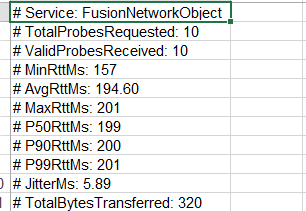
\includegraphics[width=\textwidth]{Content/Multiplayer/networkobjectbench.png}
        \caption{Bảng log CSV phương pháp Fusion Network Object}
        \label{fig:bench_netobj}
    \end{subfigure}
    \hfill
    \begin{subfigure}[b]{0.47\textwidth}
        \centering
        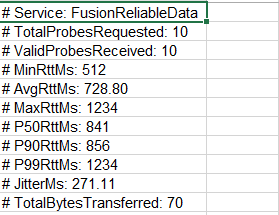
\includegraphics[width=\textwidth]{Content/Multiplayer/reliabledatabench.png}
        \caption{Bảng log CSV phương pháp Fusion Reliable Data}
        \label{fig:bench_reliable}
    \end{subfigure}
    \caption{Kết quả đo kiểm băng thông và RTT trích từ tệp log CSV thực nghiệm của hai cơ chế Photon Fusion}
    \label{fig:fusion_console_bench}
\end{figure}

\subsection{Thiết kế và hiện thực tầng hiển thị (View Layer), giao diện và hiệu ứng}

Tầng hiển thị trong \texttt{Assets/Scripts/View/} được thiết kế theo nguyên tắc \textbf{thụ động theo sự kiện (Event-Driven Presentation)}: tuyệt đối không tự tính toán luật di chuyển hay trừ AP, mà chỉ lắng nghe \texttt{GameEventBatch} từ Core thông qua giao diện \texttt{IGameEventListener} để diễn hoạt hình ảnh, âm thanh và cập nhật giao diện người dùng.

\subsubsection{Hàng đợi diễn hoạt bất đồng bộ (\texttt{VisualQueueManager} và \texttt{IVisualNode})}
Vì một lệnh duy nhất từ người chơi (ví dụ: hợp thể quân cờ, tấn công phá khiên hoặc ăn quân kích hoạt \texttt{APDrain}) có thể kéo theo chuỗi nhiều sự kiện nối tiếp nhau, hệ thống sử dụng kiến trúc hàng đợi trực quan gồm ba lớp:
\begin{itemize}
    \item \textbf{\texttt{VisualQueueManager}:} Cài đặt \texttt{IGameEventListener}, nhận từng \texttt{GameEventBatch} và thực thi tuần tự qua \texttt{UniTask} (kèm \texttt{CancellationTokenSource} tự hủy an toàn khi chuyển cảnh để tránh rò rỉ tác vụ). Đồng thời lớp này phát ra 5 sự kiện tĩnh nhẹ (\texttt{OnMatchInitialized}, \texttt{OnApUpdated}, \texttt{OnTurnChanged}, \texttt{OnPieceEliminated}, \texttt{OnGameOver}) giúp tầng HUD cập nhật tức thì mà không cần tham chiếu trực tiếp vào \texttt{MatchManager}.
    \item \textbf{\texttt{VisualSequenceBuilder} và \texttt{IVisualNode}:} Chuyển đổi các sự kiện logic thành chuỗi hành động đồ họa độc lập như \texttt{PieceMoveVisualNode} (di chuyển quân kèm vệt bóng mờ \texttt{PieceGhostTrail}), \texttt{PieceAttackVisualNode} (lao vào tấn công và kích hoạt phản hồi va chạm), \texttt{ZoomCamVisualNode} (phóng cận cảnh khi tiêu diệt quân), \texttt{CamShakedVisualNode} (rung camera tạo lực đánh) và \texttt{BoardRotatedVisualNode} (xoay bàn $180^\circ$ ở PvP Offline).
\end{itemize}

\subsubsection{Hệ thống bàn cờ, mô hình quân cờ 3D trung cổ và \texttt{PieceAnimationRelay}}
\begin{itemize}
    \item \textbf{\texttt{BoardView} và \texttt{TileView}:} Khởi tạo lưới $36$ ô cờ 3D tương ứng với chỉ số $0$--$35$ của \texttt{GameState}, hiển thị mô hình vật cản trung tuyến theo cấu hình \texttt{GameConfig}, đồng thời đổi vật liệu (material) tức thời khi rê chuột (\texttt{OnPointerHover}) và tô sáng phân biệt ô di chuyển thường, ô tấn công địch và ô hợp thể đồng minh.
    \item \textbf{Bộ 6 quân cờ 3D phong cách Trung cổ (Medieval):} Thay thế toàn bộ khối hình học tạm ban đầu bằng 6 lớp hiển thị cụ thể kế thừa từ \texttt{PieceView}: \texttt{KingPieceView}, \texttt{DarkMagePieceView}, \texttt{GreatSwordKnightPieceView}, \texttt{SwordShieldKnightPieceView}, \texttt{TraineeMagePieceView} và \texttt{VampirePieceView}. Mỗi quân cờ vận hành bằng máy trạng thái 5 pha độc lập (\texttt{IdleState}, \texttt{MoveState}, \texttt{AttackState}, \texttt{GetHitState}, \texttt{DeathState}) cùng bộ chỉ báo phe và loại quân trên không gian thế giới (\texttt{WorldCanvasPieceIndicatorService}, \texttt{SideIndicatorService}).
    \item \textbf{Cơ chế \texttt{PieceAnimationRelay} cho VFX và SFX:} Nhằm tránh lặp mã và lỗi thiếu hàm nhận sự kiện khi dùng chung Animation Clip, nhóm tái cấu trúc toàn bộ sự kiện khung hình (Animation Events) qua duy nhất một script trung chuyển \texttt{PieceAnimationRelay} gắn trên GameObject chứa \texttt{Animator}. Script này nhận chuỗi nhãn định danh (\texttt{PlayVFX}, \texttt{StopVFX}, \texttt{OnAttackSwing}, \texttt{OnHit}) từ timeline hoạt họa rồi điều phối đa hình xuống từng lớp \texttt{PieceView} cụ thể để kích hoạt đúng hiệu ứng chém, sấm sét, vỡ khiên và âm thanh qua \texttt{AudioManager} (hỗ trợ phát ngẫu nhiên/tuần tự qua \texttt{RandomAudioClipSO}, \texttt{SequenceAudioClipSO}).
\end{itemize}

\subsubsection{Kiến trúc giao diện người dùng (\texttt{UIManager}, \texttt{UIMapper} và các màn hình chính)}
Toàn bộ giao diện UGUI được chuẩn hóa tỷ lệ tự động theo độ phân giải màn hình (\texttt{CanvasScaler}) và quản lý tập trung qua cặp thành phần:
\begin{itemize}
    \item \textbf{\texttt{UIMapper} (ScriptableObject) và \texttt{UIManager}:} Đóng vai trò bảng ánh xạ nguồn chân lý duy nhất (SSOT), xây dựng sẵn hai từ điển tra cứu theo tên và theo kiểu dữ liệu \texttt{Type} tại thời điểm khởi chạy để \texttt{UIManager} bật/tắt các màn hình \texttt{UIViewBase} và hộp thoại chồng lớp \texttt{UIPopupBase} gọn gàng.
    \item \textbf{Màn hình xây dựng đội hình (\texttt{UIPopupSquadBuilder}):} Gồm bảng thẻ quân cờ (\texttt{UISquadPaletteCard}), lưới ô sân nhà (\texttt{UISquadTileSlot}) và bóng kéo thả (\texttt{UISquadDragGhost}); tự động khóa các quân vượt quá hạn mức $10$ Slot Points và phản chiếu đúng tọa độ cho cả hai phe.
    \item \textbf{Màn hình sảnh chờ trực tuyến (\texttt{UIPopupLobby}):} Cho phép chọn khu vực máy chủ Photon, tạo/vào phòng theo mã, hiển thị danh sách người chơi ở 3 nhóm Trắng -- Đen -- Khán giả, đổi slot và bật trạng thái sẵn sàng.
    \item \textbf{HUD trong trận (\texttt{UIInGameHUD}):} Hiển thị đầy đủ các chỉ số chiến thuật thiết yếu giúp người chơi ra quyết định nhanh: thanh/số lượng AP hiện tại (\texttt{UIViewAP}), lượng AP sẽ nhận ở lượt kế tiếp, nút Bỏ lượt (Pass) và số lượt Pass còn lại, chỉ báo lượt phe đang đi (\texttt{UIDualPlayerInfoPanel}, \texttt{UIPlayerHeaderWidget}) và danh sách quân cờ đã bị tiêu diệt (\texttt{UIGraveyardPanel}). Ngoài ra, hệ thống bổ sung bầu trời 3D (Skybox), ánh sáng sàn đấu và hiệu ứng chuyển cảnh mượt qua \texttt{FadeableLoader}.
\end{itemize}

\newpage

\section{Kết quả thực nghiệm và đánh giá giai đoạn 1}

Đúng với tính chất của Đồ án chuyên ngành (Giai đoạn 1), thay vì chỉ trình bày giao diện tĩnh, nhóm tập trung chạy các bộ thực nghiệm định lượng tự động trên hệ thống thực tế để kiểm chứng tính khả thi kỹ thuật của ba trụ cột cốt lõi: (i) sức mạnh và tốc độ phản hồi của hệ thống AI (tập trung vào quá trình xây dựng các thành phần nền tảng cho \textbf{Hybrid Bot} và kiểm định \textbf{LLM Bot}); (ii) hiệu quả băng thông và độ trễ của kiến trúc Multiplayer; và (iii) độ chính xác tái tạo khuôn mặt cùng tóc 3D của Smart Customization.

\subsection{Thực nghiệm đối kháng và đánh giá hệ thống AI}
Toàn bộ phép đo đối kháng AI được thực thi tự động ở chế độ mô phỏng không hiển thị đồ họa nhằm bảo đảm tốc độ và tính khách quan. Mỗi cặp đấu chạy từ $100$ đến $1{,}000$ ván đầy đủ, ghi nhận tự động tỷ lệ thắng, hòa, thua và thời gian suy nghĩ trung bình mỗi nước đi. Bảng \ref{tab:ai_benchmark_full} tổng hợp kết quả thực nghiệm qua các mốc tiến hóa thành phần tạo nên \textbf{Hybrid Bot} (từ học bắt chước, học tăng cường PPO đến kết hợp tìm kiếm Minimax và mạng đánh giá NNUE/Residual NNUE), kèm nhãn đối chiếu gọn trong ngoặc khớp với biểu đồ ở Hình \ref{fig:chart_ai_bench}.

\begin{table}[H]
    \centering
    \footnotesize
    \caption{Tổng hợp kết quả thực nghiệm đối kháng tự động giữa các mốc phát triển AI của Convergence Chess}
    \label{tab:ai_benchmark_full}
    \begin{tabularx}{\textwidth}{L{4.1cm} L{2.8cm} C{0.9cm} C{1.1cm} C{1.0cm} C{1.1cm} Y}
        \toprule
        \textbf{Mô hình thử nghiệm (P1)} & \textbf{Đối thủ chuẩn (P2)} & \textbf{Số trận} & \textbf{P1 thắng} & \textbf{Hòa} & \textbf{P2 thắng} & \textbf{Thời gian/nước (P1 vs P2)} \\
        \midrule
        Học bắt chước cơ sở (BC Template) & Minimax độ sâu 2 (Heu D2) & 100 & 1.00\% & 3.00\% & 96.00\% & -- \\
        Học bắt chước cải tiến (BC v2) & Minimax độ sâu 2 (Heu D2) & 100 & 12.00\% & 11.00\% & 77.00\% & -- \\
        Học bắt chước cải tiến (BC v2) & Minimax độ sâu 4 (Heu D4) & 100 & 18.00\% & 4.00\% & 78.00\% & -- \\
        Học tăng cường PPO tự đấu 27M bước (PPO Self-Play 27M) & Học bắt chước cơ sở (BC Template) & 100 & 87.00\% & 5.00\% & 8.00\% & -- \\
        Học tăng cường PPO tự đấu 27M bước (PPO Self-Play 27M) & Minimax độ sâu 2 (Heu D2) & 100 & 15.00\% & 6.00\% & 79.00\% & -- \\
        Học tăng cường có hàm giá trị (Critic Hybrid v4) & Minimax độ sâu 2 (Heu D2) & 1,000 & 23.90\% & 18.70\% & 57.40\% & 16 ms vs 11 ms \\
        Học tăng cường định hình thưởng (Heu RL v12p1) & Minimax độ sâu 2 (Heu D2) & 400 & 47.00\% & 26.25\% & 26.75\% & -- \\
        Học tăng cường thế hệ mới & Học tăng cường thế hệ trước & 500 & 44.80\% & 27.20\% & 28.00\% & 21 ms vs 21 ms \\
        Tìm kiếm lai mạng chính sách (NeuralMinimax) & Minimax độ sâu 2 (Heu D2) & 100 & \textbf{52.00\%} & 36.00\% & 12.00\% & 33 ms vs 6 ms \\
        Tìm kiếm lai mạng chính sách (NeuralMinimax) & Minimax độ sâu 3 (Heu D3) & 100 & \textbf{51.00\%} & 24.00\% & 25.00\% & 41 ms vs 10 ms \\
        Tìm kiếm lai mạng chính sách (NeuralMinimax) & Minimax độ sâu 4 (Heu D4) & 100 & 37.00\% & 30.00\% & 33.00\% & 38 ms vs 28 ms \\
        Mạng NNUE thế hệ 7, độ sâu 4 (NNUE Gen7) & Minimax độ sâu 4 (Heu D4) & 100 & 23.00\% & 49.00\% & 28.00\% & 238 ms vs 21 ms \\
        Hybrid Bot thế hệ 7 (NNUE + PPO) & Hybrid Bot thế hệ 3 & 100 & 33.00\% & 47.00\% & 20.00\% & 210 ms vs 218 ms \\
        \textbf{Mạng NNUE dạng dư thế hệ 7, độ sâu 4 (Residual NNUE Gen7)} & \textbf{Minimax độ sâu 4 (Heu D4)} & \textbf{100} & \textbf{51.00\%} & \textbf{28.00\%} & \textbf{21.00\%} & \textbf{66 ms vs 4 ms} \\
        Minimax độ sâu 1 (Heu D1) & Minimax độ sâu 6 (Heu D6) & 100 & 12.00\% & 10.00\% & 78.00\% & 6 ms vs 536 ms \\
        \bottomrule
    \end{tabularx}
\end{table}

\begin{figure}[H]
    \centering
    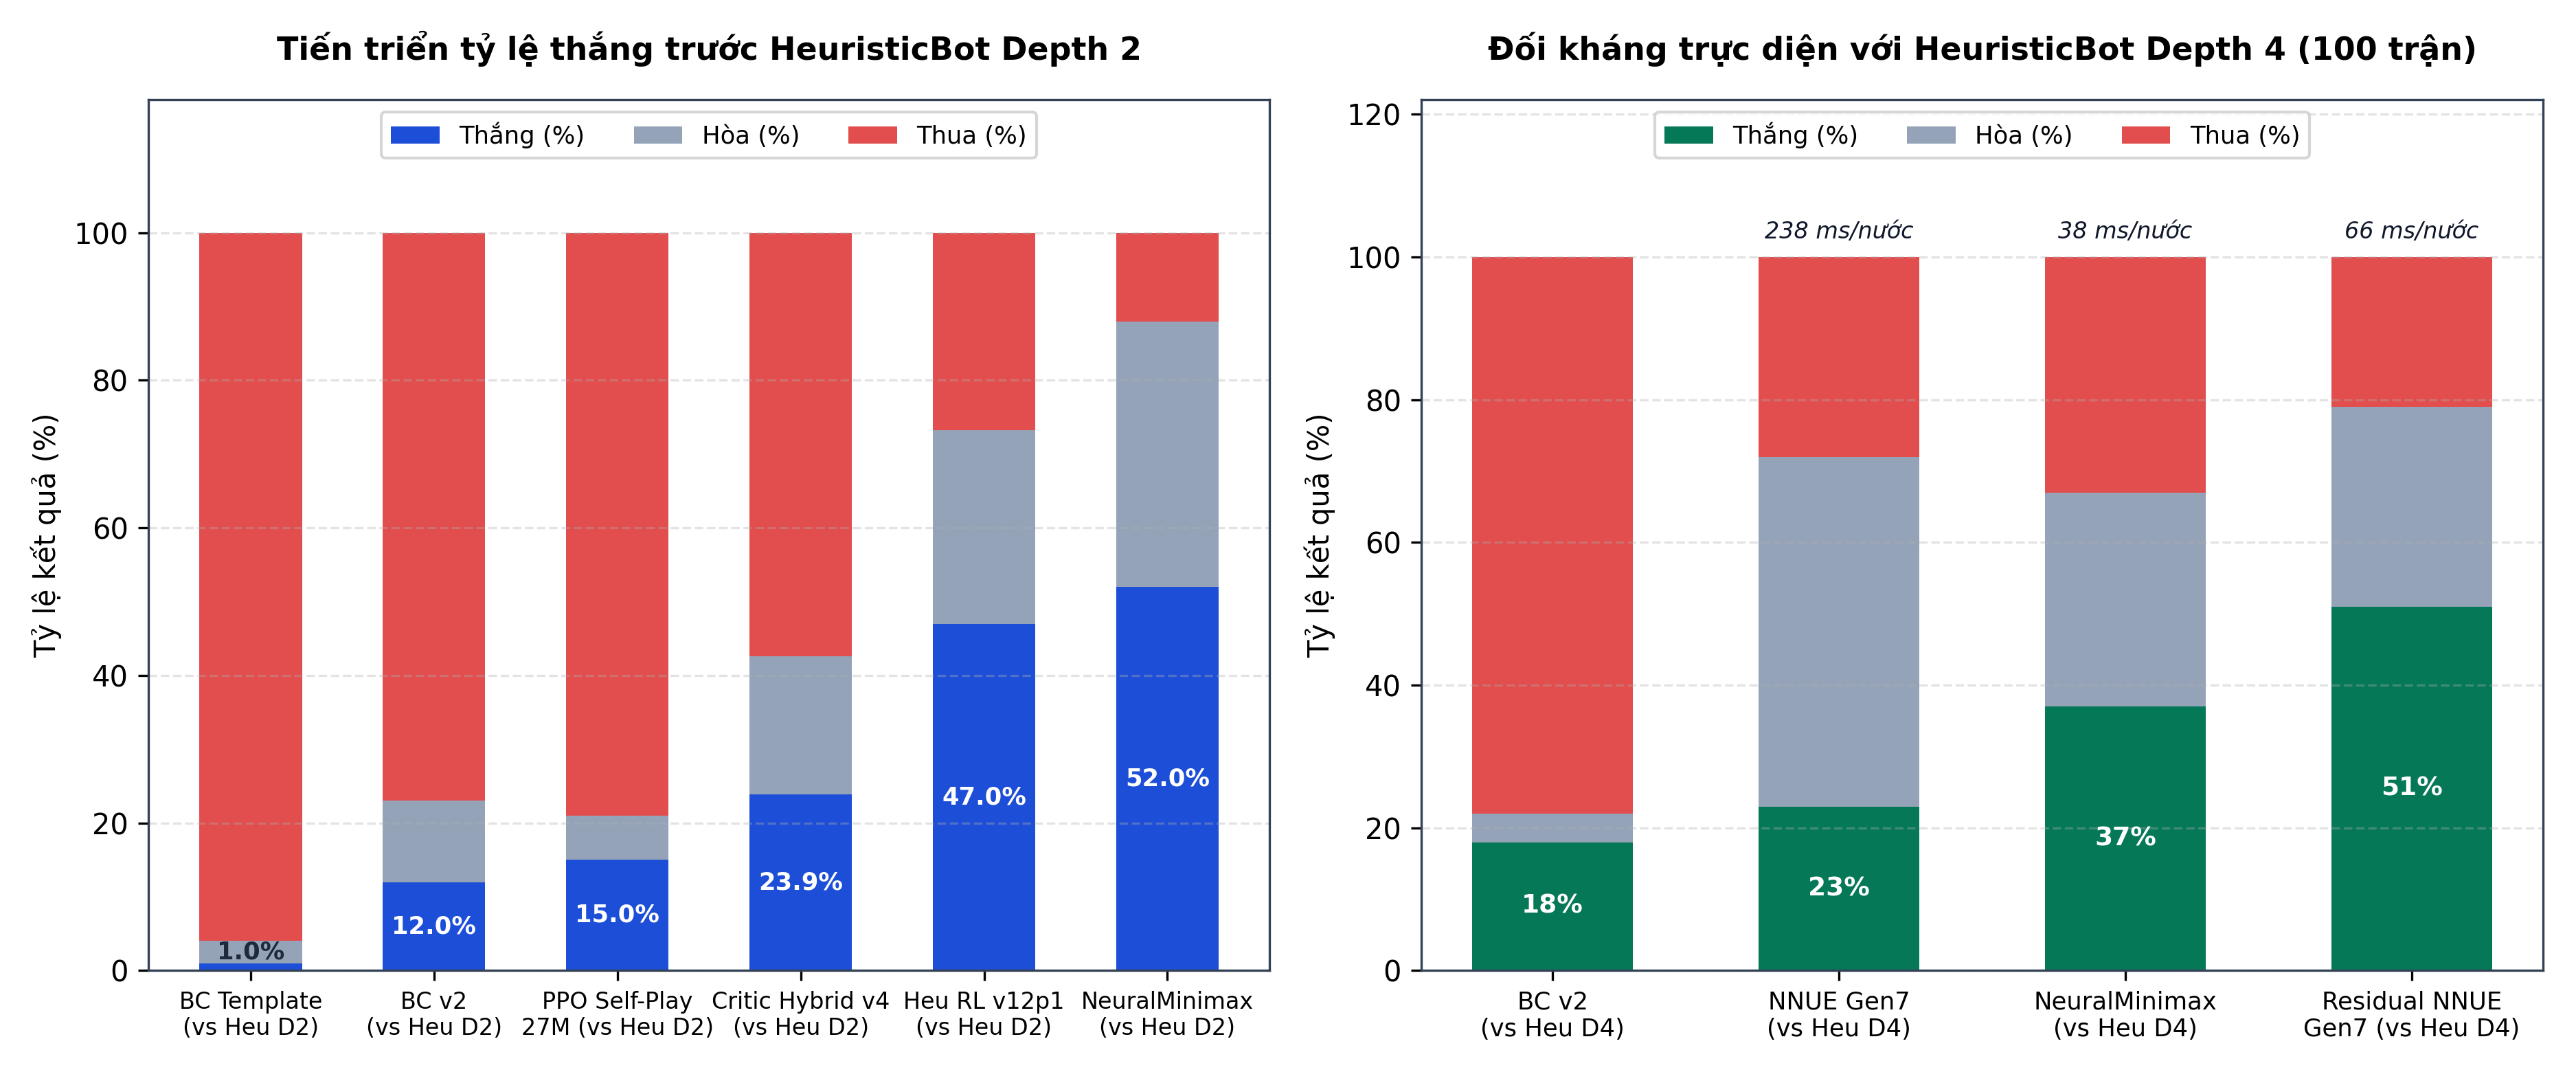
\includegraphics[width=\textwidth]{Diagrams/images/chart_ai_benchmark.png}
    \caption{Biểu đồ tiến triển tỷ lệ thắng của các mốc phát triển AI trước Minimax độ sâu 2 và độ sâu 4}
    \label{fig:chart_ai_bench}
\end{figure}

Từ Bảng \ref{tab:ai_benchmark_full} và Hình \ref{fig:chart_ai_bench}, nhóm rút ra bốn kết luận khoa học làm cơ sở định hình \textbf{Hybrid Bot} và \textbf{LLM Bot} sang Giai đoạn 2:
\begin{enumerate}
    \item \textbf{Giới hạn của mạng chính sách thuần túy không có tìm kiếm cây:} Dù mô hình học tăng cường PPO tự đấu áp đảo bản học bắt chước khởi tạo ($87.0\%$ so với $8.0\%$) và phản hồi rất nhanh (khoảng $16$--$21$ mili-giây mỗi nước), mạng chỉ nhìn một nước đi vẫn dễ mắc sai lầm chiến thuật ngắn hạn trước cây tìm kiếm Minimax do luật hợp thể và Surge tạo ra chuỗi ăn quân nhiều bước. Khi bổ sung định hình phần thưởng (Heu RL v12p1), tỷ lệ thắng trước Minimax độ sâu 2 tăng mạnh từ $15.0\%$ lên $47.0\%$ (vượt xa tỷ lệ thua $26.75\%$).
    \item \textbf{Hiệu quả rõ rệt của kiến trúc lai tìm kiếm và học sâu:} Khi dùng xác suất ưu tiên nước đi từ mạng chính sách dẫn đường cho cây tìm kiếm Minimax (NeuralMinimax), tác nhân áp đảo cả Minimax độ sâu 2 ($52\%$ thắng -- $12\%$ thua) lẫn độ sâu 3 ($51\%$ thắng -- $25\%$ thua) và nhỉnh hơn độ sâu 4 ($37\%$ -- $33\%$) chỉ với thời gian suy nghĩ $38$ mili-giây mỗi nước.
    \item \textbf{Bước đột phá của mạng đánh giá NNUE dạng dư trong Hybrid Bot:} So với mạng NNUE chuẩn cùng thế hệ dữ liệu thứ 7 ($23\%$ thắng, $238$ mili-giây mỗi nước), biến thể \textbf{NNUE dạng dư (Residual NNUE Gen7)} nâng tỷ lệ thắng trước Minimax độ sâu 4 lên tới \textbf{51.00\%} (chỉ thua $21.00\%$) đồng thời giảm thời gian suy nghĩ xuống còn \textbf{66 mili-giây mỗi nước} (nhanh hơn $3.6$ lần nhờ thứ tự đánh giá nút lá chính xác giúp cắt tỉa Alpha-Beta hiệu quả hơn).
    \item \textbf{Hiệu quả vòng lặp đồng huấn luyện đa thế hệ và kiểm định LLM Bot:} Phiên bản \textbf{Hybrid Bot thế hệ 7} đánh bại thế hệ 3 với tỷ số $33\%$ thắng -- $20\%$ thua ($47\%$ hòa), khẳng định hiệu quả của cơ chế tự sinh dữ liệu qua nhiều thế hệ. Song song đó, quy trình tiến hóa \textbf{LLM Bot} đã sàng lọc thành công $5$ mô-đun quy tắc chiến thuật vượt qua đủ $4$ cổng kiểm định tự động về tính an toàn, tốc độ, tính đối xứng và hiệu quả đối kháng cặp.
\end{enumerate}

\subsection{Đánh giá thực nghiệm hệ thống Multiplayer (Photon Fusion)}
Hình \ref{fig:chart_net_bench} trực quan hóa sự đánh đổi giữa băng thông và độ trễ từ phép đo 10 lần thăm dò trên Photon Fusion. Giao thức nhị phân tùy biến \texttt{OnlineDataBroadcastNetwork} trên kênh \texttt{Fusion Reliable Data} cắt giảm \textbf{78.1\%} tổng lưu lượng truyền tải (chỉ $70$ bytes so với $320$ bytes của \texttt{NetworkObject}) trong khi giữ tách biệt hoàn toàn với Core Domain. Các kịch bản kiểm thử đồng bộ giữa 2 máy khách và Khán giả (Spectator) đã xác nhận đồng bộ chính xác tên người chơi, danh sách slot, đội hình (\texttt{SquadData}), trạng thái sẵn sàng, hạt giống vật cản trung tuyến và luồng nước đi 4 bytes.

\begin{figure}[H]
    \centering
    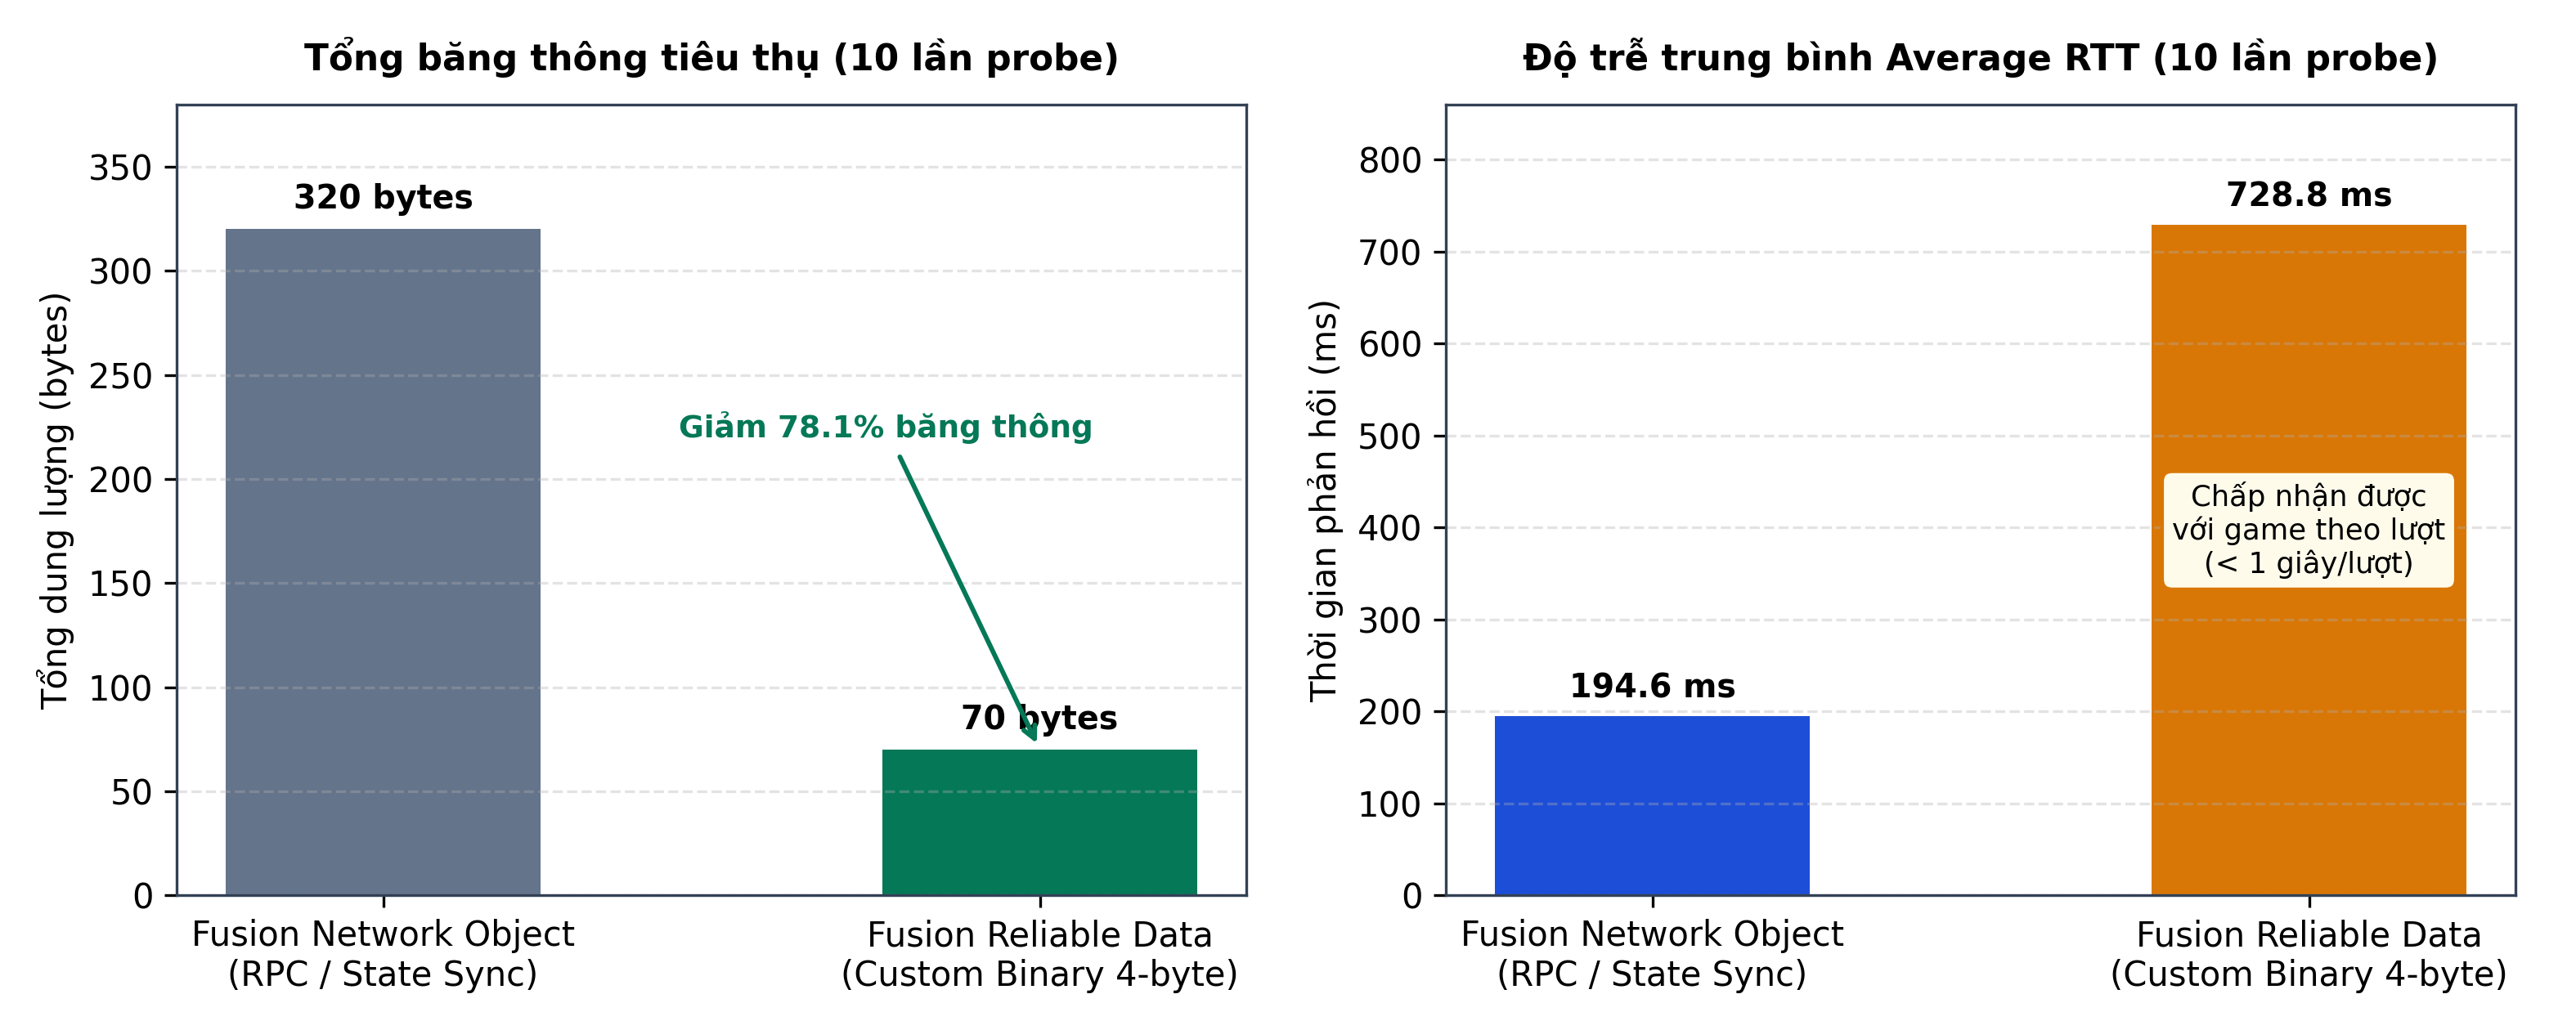
\includegraphics[width=0.95\textwidth]{Diagrams/images/chart_network_benchmark.png}
    \caption{So sánh định lượng băng thông tiêu thụ và Average RTT giữa hai cơ chế Photon Fusion}
    \label{fig:chart_net_bench}
\end{figure}

\subsection{Đánh giá thực nghiệm phân hệ tùy biến nhân vật 3D (Smart Customization)}
Trên máy trạm có cạc đồ họa NVIDIA GeForce RTX 4050 Laptop (bộ nhớ đồ họa 6 GB), quy trình tùy biến nhân vật 3D đã đạt được các kết quả kiểm chứng thực tế sau:
\begin{itemize}
    \item \textbf{Độ chính xác hình học khuôn mặt:} Sau khi tinh gọn về $25$ thông số hình thái độc lập và kiểm soát góc chụp khi sinh $24{,}000$ mẫu tổng hợp ($12{,}000$ Nam và $12{,}000$ Nữ), sai số tuyệt đối trung bình trên tập kiểm định sau $80$ chu kỳ huấn luyện giảm từ $0.0749$ ở phiên bản đầu xuống còn \textbf{0.0621} đối với mẫu Nam và \textbf{0.0616} đối với mẫu Nữ.
    \item \textbf{Chất lượng bề mặt da, khử bóng và thời gian xử lý:} Kết hợp chiếu ngược tam giác trên PyTorch3D kiểu MeInGame \cite{meingame}, khử bóng đối xứng hai bên trong không gian màu Lab, tách vùng hốc mắt, lọc bỏ vệt men răng và hòa trộn biên đa tầng (vùng chuyển tiếp $64$ điểm ảnh) giúp loại bỏ viền ghép gò má -- cổ và tránh hiện tượng bề mặt da bị bệt mờ như tượng sáp. Tổng thời gian xử lý toàn trình cho một ảnh chân dung ở chế độ tiêu chuẩn đạt khoảng \textbf{5.9 giây} trên máy tính cục bộ.
    \item \textbf{Hiệu quả hiển thị 3D trong Unity 6:} Hệ thống $6$ kiểu tóc 3D khớp chính xác vào da đầu, vật liệu mắt tạo đốm sáng tự nhiên trên giác mạc và bản đồ chi tiết nếp nhăn HRN có thể tinh chỉnh độ sâu trực tiếp trong trò chơi như minh họa tại Hình \ref{fig:sc_results}.
\end{itemize}

\begin{figure}[H]
    \centering
    \begin{subfigure}[b]{0.31\textwidth}
        \centering
        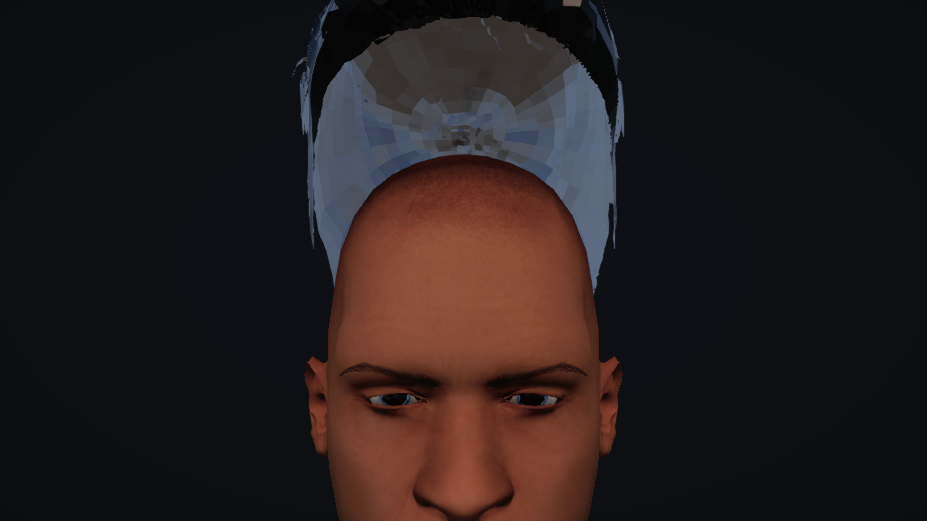
\includegraphics[width=\textwidth]{Content/Thực nghiệm và đánh giá/images/sc_hair_male_short01.png}
        \caption{Mẫu Nam kèm tóc ngắn kiểu 1}
    \end{subfigure}
    \hfill
    \begin{subfigure}[b]{0.31\textwidth}
        \centering
        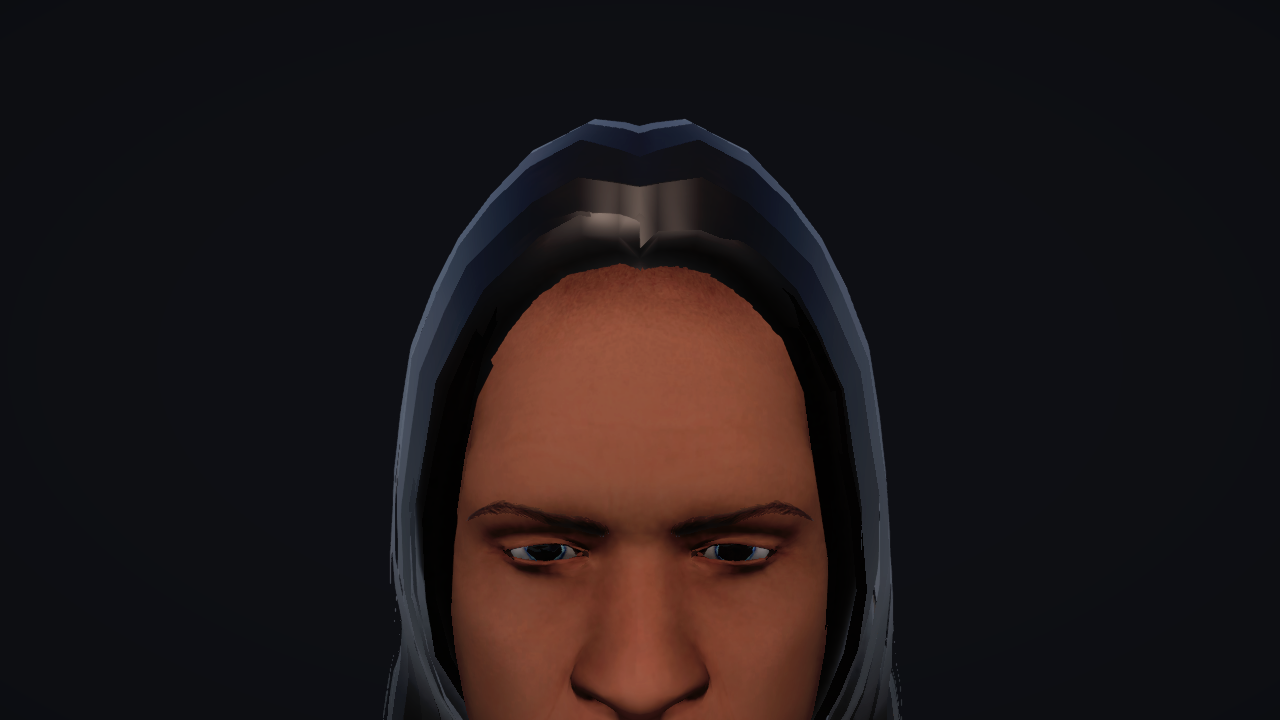
\includegraphics[width=\textwidth]{Content/Thực nghiệm và đánh giá/images/sc_hair_long01_verified.png}
        \caption{Mẫu Nữ kèm tóc dài}
    \end{subfigure}
    \hfill
    \begin{subfigure}[b]{0.31\textwidth}
        \centering
        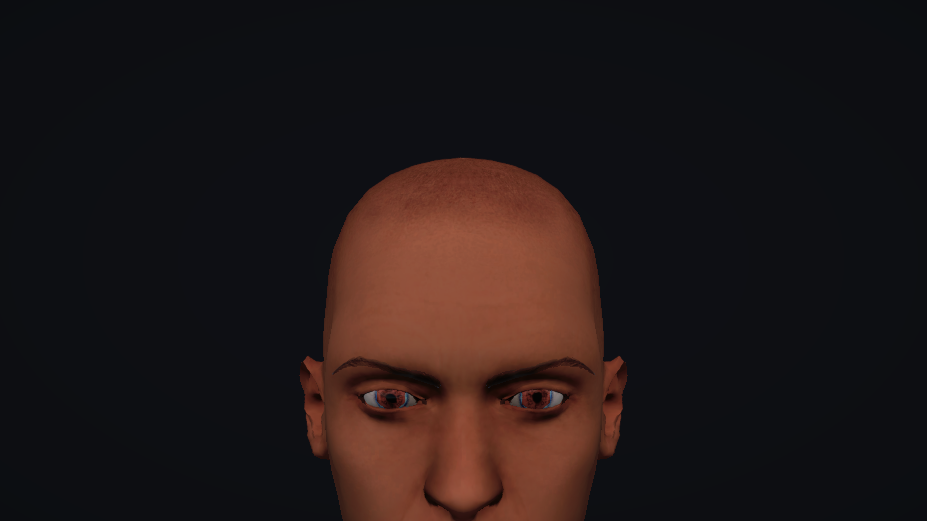
\includegraphics[width=\textwidth]{Content/Thực nghiệm và đánh giá/images/sc_hair_test_obama.png}
        \caption{Kiểm chứng tái tạo từ ảnh chân dung thực tế}
    \end{subfigure}
    \caption{Kết quả thực nghiệm tái tạo khuôn mặt, khử bóng da, vật liệu mắt và gắn tóc 3D trong Unity 6}
    \label{fig:sc_results}
\end{figure}

\begin{notebox}{Các hướng tiếp cận đã kiểm chứng loại bỏ hoặc tạm dừng trong giai đoạn 1}
Một giá trị thực nghiệm quan trọng của giai đoạn Đồ án chuyên ngành là sớm phát hiện và loại bỏ các phương án kém hiệu quả để tránh lãng phí nguồn lực ở Giai đoạn 2:
\begin{enumerate}
    \item \textbf{Dùng trực tiếp chiều sâu ước lượng từ MediaPipe:} Gây sai số trung bình bình phương tới $0.1415$ theo khoảng cách hai mắt (gấp $2.5$ lần sai số chiều ngang), buộc phải chuyển sang phương pháp sinh dữ liệu phối cảnh tổng hợp trực tiếp từ mô hình 3D gốc.
    \item \textbf{Huấn luyện mạng sinh kết cấu da trên dữ liệu tổng hợp:} Gây hiện tượng loang màu hồng nhân tạo quanh miệng và làm bề mặt da bệt mờ như tượng sáp; đã loại bỏ khỏi quy trình chính.
    \item \textbf{Khử bóng bằng mô hình khuếch tán IC-Light \cite{iclight}:} Dù khử bóng tốt (tốn khoảng $1.8$ giây riêng bước khuếch tán), mô hình này phụ thuộc bộ trọng số nặng và có nguy cơ làm thay đổi nét nhận dạng khuôn mặt gốc, do đó đã được tạm dừng để thay bằng chiếu ngược PyTorch3D kết hợp khử bóng đối xứng thuần giải phẫu.
    \item \textbf{Chuyển đổi trực tiếp bản đồ chi tiết bề mặt giữa hai chuẩn khuôn mặt khác nhau:} Gây đảo hướng ánh sáng tiếp tuyến do khác biệt góc xoay hệ tọa độ bề mặt; đã khắc phục bằng cách chuyển đổi bản đồ độ cao trước rồi mới tính lại độ dốc bề mặt trên hệ tọa độ của nhân vật đích.
    \item \textbf{Gắn trực tiếp mô hình tóc rời bằng khung xương mặc định hoặc dịch tọa độ thủ công:} Gây lệch tư thế gốc khiến tóc bị rơi xuống thấp hoặc chìm $4$--$5$ cm vào trong hộp sọ; đã chuẩn hóa hoàn toàn bằng công cụ định vị da đầu của MPFB v2.
\end{enumerate}
\end{notebox}

\subsection{Kết quả giao diện nguyên mẫu các màn hình trò chơi}
Bên cạnh các kết quả định lượng về AI, mạng và Smart Customization, nguyên mẫu chơi thử đã kết nối hoàn chỉnh các màn hình điều hướng chính trong Unity 6. Ba khung hình dưới đây đánh dấu các góc chụp giao diện thực tế từ bản dựng hiện tại để nhóm bổ sung ảnh chụp màn hình trước khi in nộp:

\begin{figure}[H]
    \centering
    \screenshotplaceholder{Content/Thực nghiệm và đánh giá/images/ui\_mainmenu\_squad.png}{Chụp ảnh màn hình chính và giao diện xây dựng đội hình đang kéo thả quân cờ trong ngân sách 12 điểm.}
    \caption{Giao diện màn hình chính và màn hình thiết lập đội hình}
    \label{fig:ui_squad_placeholder}
\end{figure}

\begin{figure}[H]
    \centering
    \screenshotplaceholder{Content/Thực nghiệm và đánh giá/images/ui\_lobby\_online.png}{Chụp ảnh màn hình sảnh chờ PvP Online (UIPopupLobby) thể hiện lựa chọn Photon Region, mã phòng, 3 nhóm vị trí (Trắng, Đen, Khán giả) và trạng thái Sẵn sàng.}
    \caption{Giao diện sảnh chờ PvP Online hỗ trợ phân vai và đồng bộ đội hình}
    \label{fig:ui_lobby_placeholder}
\end{figure}

\begin{figure}[H]
    \centering
    \screenshotplaceholder{Content/Thực nghiệm và đánh giá/images/ui\_ingame\_6x6.png}{Chụp ảnh trận đấu thực tế trên bàn cờ 3D 6x6 gồm bộ quân cờ Trung cổ, ô vật cản trung tuyến, vùng tô sáng nước đi/hợp thể và bảng thông số trong trận.}
    \caption{Giao diện bàn cờ 3D 6x6 và bảng thông số chiến thuật trong trận đấu}
    \label{fig:ui_ingame_placeholder}
\end{figure}

\newpage
\section{Tiến độ thực hiện giai đoạn 1 và kế hoạch giai đoạn 2}

\subsection{Tổng kết tiến độ 15 tuần của giai đoạn 1 (DACN)}
Để bảo đảm tính minh bạch và trung thực đối chiếu giữa kế hoạch đề ra ban đầu với mã nguồn thực tế tại thời điểm kết thúc Giai đoạn 1 (DACN), Bảng \ref{tab:stage1_progress} đối chiếu chi tiết từng tuần công việc theo ba trạng thái: \textbf{Hoàn thành}, \textbf{Mở rộng vượt kế hoạch} (các hướng nghiên cứu chuyên sâu đã hiện thực và kiểm chứng trong repo) và \textbf{Chuyển sang Giai đoạn 2 (DATN)} (các tính năng mang tính vận hành sản phẩm quy mô lớn).

\begin{longtable}{C{1.3cm} L{5.4cm} L{5.5cm} C{2.6cm}}
    \caption{Đối chiếu kế hoạch thực hiện 15 tuần giai đoạn 1 (DACN) với kết quả thực tế}
    \label{tab:stage1_progress} \\
    \toprule
    \textbf{Tuần} & \textbf{Kế hoạch đề ra (Giai đoạn 1)} & \textbf{Kết quả thực tế ghi nhận trong codebase} & \textbf{Trạng thái} \\
    \midrule
    \endfirsthead
    \toprule
    \textbf{Tuần} & \textbf{Kế hoạch đề ra (Giai đoạn 1)} & \textbf{Kết quả thực tế ghi nhận trong codebase} & \textbf{Trạng thái} \\
    \midrule
    \endhead
    \bottomrule
    \endfoot

    Tuần 1 & Dựng bản mẫu bàn cờ $6 \times 6$, AP, di chuyển, hợp thể, sinh vật cản ngẫu nhiên và kiểm tra nước đi. & Hoàn thiện nhân C\# thuần: \texttt{GameState}, \texttt{MoveValidator}, \texttt{PassiveFlags} (9-bit), sinh $1$--$2$ vật cản trung tuyến, Surge Phase. & Hoàn thành \\
    \midrule
    Tuần 2 & Tách cấu hình, PvP Offline, highlight/rung/zoom camera và Minimax Alpha-Beta cơ bản. & Hoàn thiện \texttt{GameConfig} ScriptableObject, \texttt{PvPOffModeBootstrapper}, \texttt{BoardRotator}, \texttt{CamShaked}/\texttt{ZoomCam}, \texttt{MinimaxSearch}. & Hoàn thành \\
    \midrule
    Tuần 3 & Squad Builder $10$ Slots, điều kiện kết thúc, mô phỏng hàng loạt tìm lỗi kẹt cờ, khảo sát Photon. & Hoàn thiện \texttt{UIPopupSquadBuilder}, \texttt{SquadValidator}, \texttt{SaveLoadManager}, tích hợp Photon Fusion 2. & Hoàn thành \\
    \midrule
    Tuần 4 & Kết nối mạng 2 máy (region, phòng, đồng bộ đội hình, timer) và bắt đầu huấn luyện ML-Agents. & Hiện thực \texttt{OnlineSessionManager}, \texttt{OnlineDataBroadcastNetwork}, \texttt{OnlineTurnTimer}, \texttt{AgentBotController} + BC/PPO. & Hoàn thành \\
    \midrule
    Tuần 5 & Thay mô hình 3D Trung cổ, dựng Scene benchmark đối kháng AI, sửa lỗi đồng bộ Ready/Tên Online. & Tích hợp 6 quân cờ 3D Medieval, hoàn thiện \texttt{BenchmarkBootstrapper} + \texttt{FileBenchmarkRecorder}, sửa đồng bộ tên/Ready. & Hoàn thành \\
    \midrule
    Tuần 6 & Thử nghiệm AI Hybrid (ML + Minimax), animation Idle/Move/Attack, dựng lại UI Main Menu/Lobby/HUD. & Hiện thực \texttt{HybridAgentBotController}, \texttt{NeuralMinimaxBotController}, FSM quân cờ và bộ giao diện UGUI qua \texttt{UIMapper}. & Hoàn thành \\
    \midrule
    Tuần 7 & Animation GetHit/Death, VFX đòn đánh, zoom camera khi ăn quân, nâng cấp bàn cờ 3D. & Hoàn thiện 5 trạng thái \texttt{PieceView}, chuẩn hóa \texttt{PieceAnimationRelay}, nâng cấp bàn cờ 3D và \texttt{PieceGhostTrail}. & Hoàn thành \\
    \midrule
    Tuần 8 & Hệ thống âm thanh SFX/BGM, cân chỉnh Skybox/ánh sáng và khởi động nghiên cứu SC (Nam/Nữ). & Hiện thực \texttt{AudioManager}, Skybox/lighting URP, chuẩn bị base mesh Nam/Nữ trên MPFB v2 (Blender 4.2). & Hoàn thành \\
    \midrule
    Tuần 9 & Thử nghiệm nắn hình học 3D từ ảnh 2D, xử lý màu da/UV và xem trước trong Unity. & Xây dựng pipeline Python FastAPI + \texttt{SCCharacterCreator}, kiểm chứng loại bỏ hướng Z-MediaPipe và \texttt{sc\_texnet}. & Hoàn thành \\
    \midrule
    Tuần 10 & Đưa giao diện SC vào game kèm thanh trượt thủ công và nghiên cứu khử bóng Texture (delighting). & Hiện thực \texttt{SCCanvasUI}, \texttt{SCBlendShapeRow}, tích hợp IC-Light FP16 ($\sim 1.8$s) và Method B1 v2 ($25$ kênh trực giao). & Hoàn thành \\
    \midrule
    Tuần 11 & Làm mượt biên cổ (seam blending), hạn chế méo UV và kiểm tra chuyển đổi Nam -- Nữ. & Hoàn thiện chiếu Barycentric PyTorch3D, Hermite $64$px, HRN Normal Map, mắt PBR Catchlight và \textbf{bổ sung 6 kiểu tóc 3D MPFB v2}. & Mở rộng vượt kế hoạch \\
    \midrule
    Tuần 12 & Mở rộng tự đấu AI, kiểm tra ổn định mạng (desync/lag); \textit{thêm tìm trận tự động, đấu hạng, Elo}. & Hoàn thiện \textbf{NNUE, Residual NNUE ($51\%$ thắng D4), ObservationEncoderV2 ($654$f) và LLM Evolved Module Bank}; chạy benchmark $10$ probes mạng. Hạng mục Matchmaking/Elo dời sang DATN. & Mở rộng AI; dời Elo sang DATN \\
    \midrule
    Tuần 13 & Mô phỏng cân bằng đi trước/đi sau, rà soát tình huống biên AP/Hợp thể, VFX; \textit{bảng xếp hạng, bạn bè}. & Xử lý race condition Attack/Move, kiểm thử hàng trăm ván tự đấu AI; hoàn thiện bộ VFX sấm sét/va chạm. Hạng mục Bảng xếp hạng và Bạn bè dời sang DATN. & Hoàn thành Core/AI; dời Social sang DATN \\
    \midrule
    Tuần 14 & Ghép luồng cài đặt, thử nghiệm lưu dữ liệu, đo hiệu năng khung hình và bộ nhớ. & Hoàn thiện \texttt{UIPopupSettings}, \texttt{SaveLoadManager} (\texttt{SquadSLO}, \texttt{GeneralSettingsSLO}), kiểm tra tốc độ suy nghĩ AI ($<70$ ms). & Hoàn thành cơ bản \\
    \midrule
    Tuần 15 & Chơi thử tìm lỗi góc chết, tổng hợp danh sách lỗi và dựng bản cài đặt mẫu PC. & Tổng hợp danh sách lỗi/hạn chế cho Giai đoạn 2, hoàn thiện tài liệu kiến trúc và báo cáo tổng kết Giai đoạn 1 (DACN). & Hoàn thành \\
\end{longtable}

\subsection{Tổng kết đóng góp của từng thành viên trong giai đoạn 1}
Bảng \ref{tab:member_contrib} ghi nhận đóng góp thực tế của hai thành viên căn cứ theo lịch sử commit Git (tổng cộng hơn $260$ commit tính đến tháng 11/2026).

\begin{table}[H]
    \centering
    \caption{Bảng tổng kết phân công và đóng góp của thành viên trong giai đoạn 1 (DACN)}
    \label{tab:member_contrib}
    \begin{tabularx}{\textwidth}{L{3.2cm} Y C{2.2cm}}
        \toprule
        \textbf{Thành viên} & \textbf{Các hạng mục kỹ thuật chủ trì và hoàn thành} & \textbf{Tỷ trọng} \\
        \midrule
        Thành viên 1 (Chủ trì Core, AI và SC) & Kiến trúc Hexagonal và \texttt{ArenaServiceLocator}; toàn bộ Core Domain (\texttt{GameState}, \texttt{MoveValidator}, \texttt{MatchManager}, \texttt{PassiveFlags}); toàn bộ hệ sinh thái AI (Minimax/PVS/Zobrist, BC/DAgger, PPO Self-Play, \texttt{ObservationEncoderV2}, NNUE/Residual NNUE, Hybrid Bot, LLM FunSearch); toàn bộ pipeline Smart Customization (Method B1 v2, IC-Light, PyTorch3D, HRN, 3D Hair, PBR Eyes); \texttt{PieceAnimationRelay} và hệ thống Benchmark tự động. & 50\% \\
        \midrule
        Thành viên 2 -- Đăng (Chủ trì Multiplayer và View Layer) & Khảo sát và triển khai Multiplayer trên Photon Fusion (\texttt{OnlineSessionManager}, \texttt{OnlineDataBroadcastNetwork}, 9 \texttt{BroadcastDataHandler}, \texttt{NetworkController}, \texttt{OnlineLocalMoveSender}, \texttt{OnlineTurnTimer}, đo benchmark NetworkObject vs Reliable Data); PvP Offline (\texttt{BoardRotator}); tầng View (\texttt{BoardView}, \texttt{TileView}, \texttt{PieceView} 3D, \texttt{VisualQueueManager}); toàn bộ hệ thống UI (\texttt{UIManager}, \texttt{UIMapper}, \texttt{UIPopupSquadBuilder}, \texttt{UIPopupLobby}, \texttt{UIInGameHUD}); tích hợp VFX/SFX và Skybox. & 50\% \\
        \bottomrule
    \end{tabularx}
\end{table}

\subsection{Đánh giá chung và các hạn chế còn tồn tại}
Kết thúc Giai đoạn 1 (DACN), nhóm đã chứng minh trọn vẹn tính khả thi kỹ thuật của cả bốn mảng phức tạp nhất: lõi cờ chiến thuật $6 \times 6$ tách rời hoàn toàn khỏi Unity, AI lai \texttt{Residual NNUE} vượt trội Heuristic Depth 4 ở thời gian phản hồi $66$ ms, giao thức mạng nhị phân 4-byte trên Photon Fusion tiết kiệm $78.1\%$ băng thông và pipeline tạo khuôn mặt/tóc 3D từ ảnh chân dung chạy thực tế trên GPU tầm trung.

Tuy nhiên, do phạm vi DACN tập trung vào khảo sát, kiến trúc và nguyên mẫu, sản phẩm hiện vẫn còn năm hạn chế chính cần giải quyết triệt để ở Giai đoạn 2:
\begin{enumerate}
    \item \textbf{Chưa hoàn thiện xử lý sự cố mạng và tài khoản người chơi:} Hệ thống Multiplayer hiện chưa có cơ chế tự động kết nối lại (Reconnect) sau khi đứt mạng giữa trận, chưa xử lý triệt để mọi tình huống hết giờ/rời phòng đột ngột và chưa tích hợp xác thực tài khoản (Google/Facebook) hay cơ sở dữ liệu đám mây.
    \item \textbf{Chưa có hệ thống cạnh tranh xã hội:} Các tính năng ghép trận tự động (Matchmaking), tính điểm xếp hạng Elo, bảng xếp hạng toàn cục (Leaderboard) và danh sách bạn bè mới dừng ở mức thiết kế kế hoạch.
    \item \textbf{Triển khai Smart Customization còn phụ thuộc môi trường Python cục bộ:} Backend FastAPI hiện chạy trên máy trạm phát triển có GPU RTX 4050; cần phương án đóng gói dịch vụ hoặc triển khai máy chủ suy luận (hoặc rút gọn ONNX chạy trực tiếp trên thiết bị) khi phát hành cho người dùng cuối.
    \item \textbf{Chưa cài đặt quy tắc hòa lặp thế cờ 3 lần (Threefold Repetition):} Hiện chỉ mới giới hạn hòa theo \texttt{MaxTurns = 60} và giới hạn lượt Pass.
    \item \textbf{Chưa tiến hành tối ưu hiệu năng sâu và kiểm thử người dùng quy mô lớn:} Chưa tối ưu Draw Calls/GPU Instancing, chưa có hướng dẫn tân thủ tương tác (Interactive Tutorial) cho luật hợp thể + Surge và chưa thu thập dữ liệu khảo sát trải nghiệm từ người chơi thực tế.
\end{enumerate}

\subsection{Kế hoạch triển khai giai đoạn 2 -- Đồ án tốt nghiệp (DATN)}
Nếu Giai đoạn 1 (DACN) là chặng \textit{nghiên cứu, đánh giá và chứng minh nguyên mẫu}, thì \textbf{Giai đoạn 2 (DATN -- dự kiến 16 tuần, từ Tuần 16 đến Tuần 31)} hướng thẳng tới mục tiêu \textbf{hoàn thiện sản phẩm đạt chất lượng phát hành công khai (Production-ready Release)} trên nền tảng PC (itch.io / Steam Demo). Hình \ref{fig:roadmap_gantt} và Bảng \ref{tab:stage2_plan} mô tả lộ trình chuyển tiếp liền mạch giữa hai giai đoạn.

\begin{figure}[H]
    \centering
    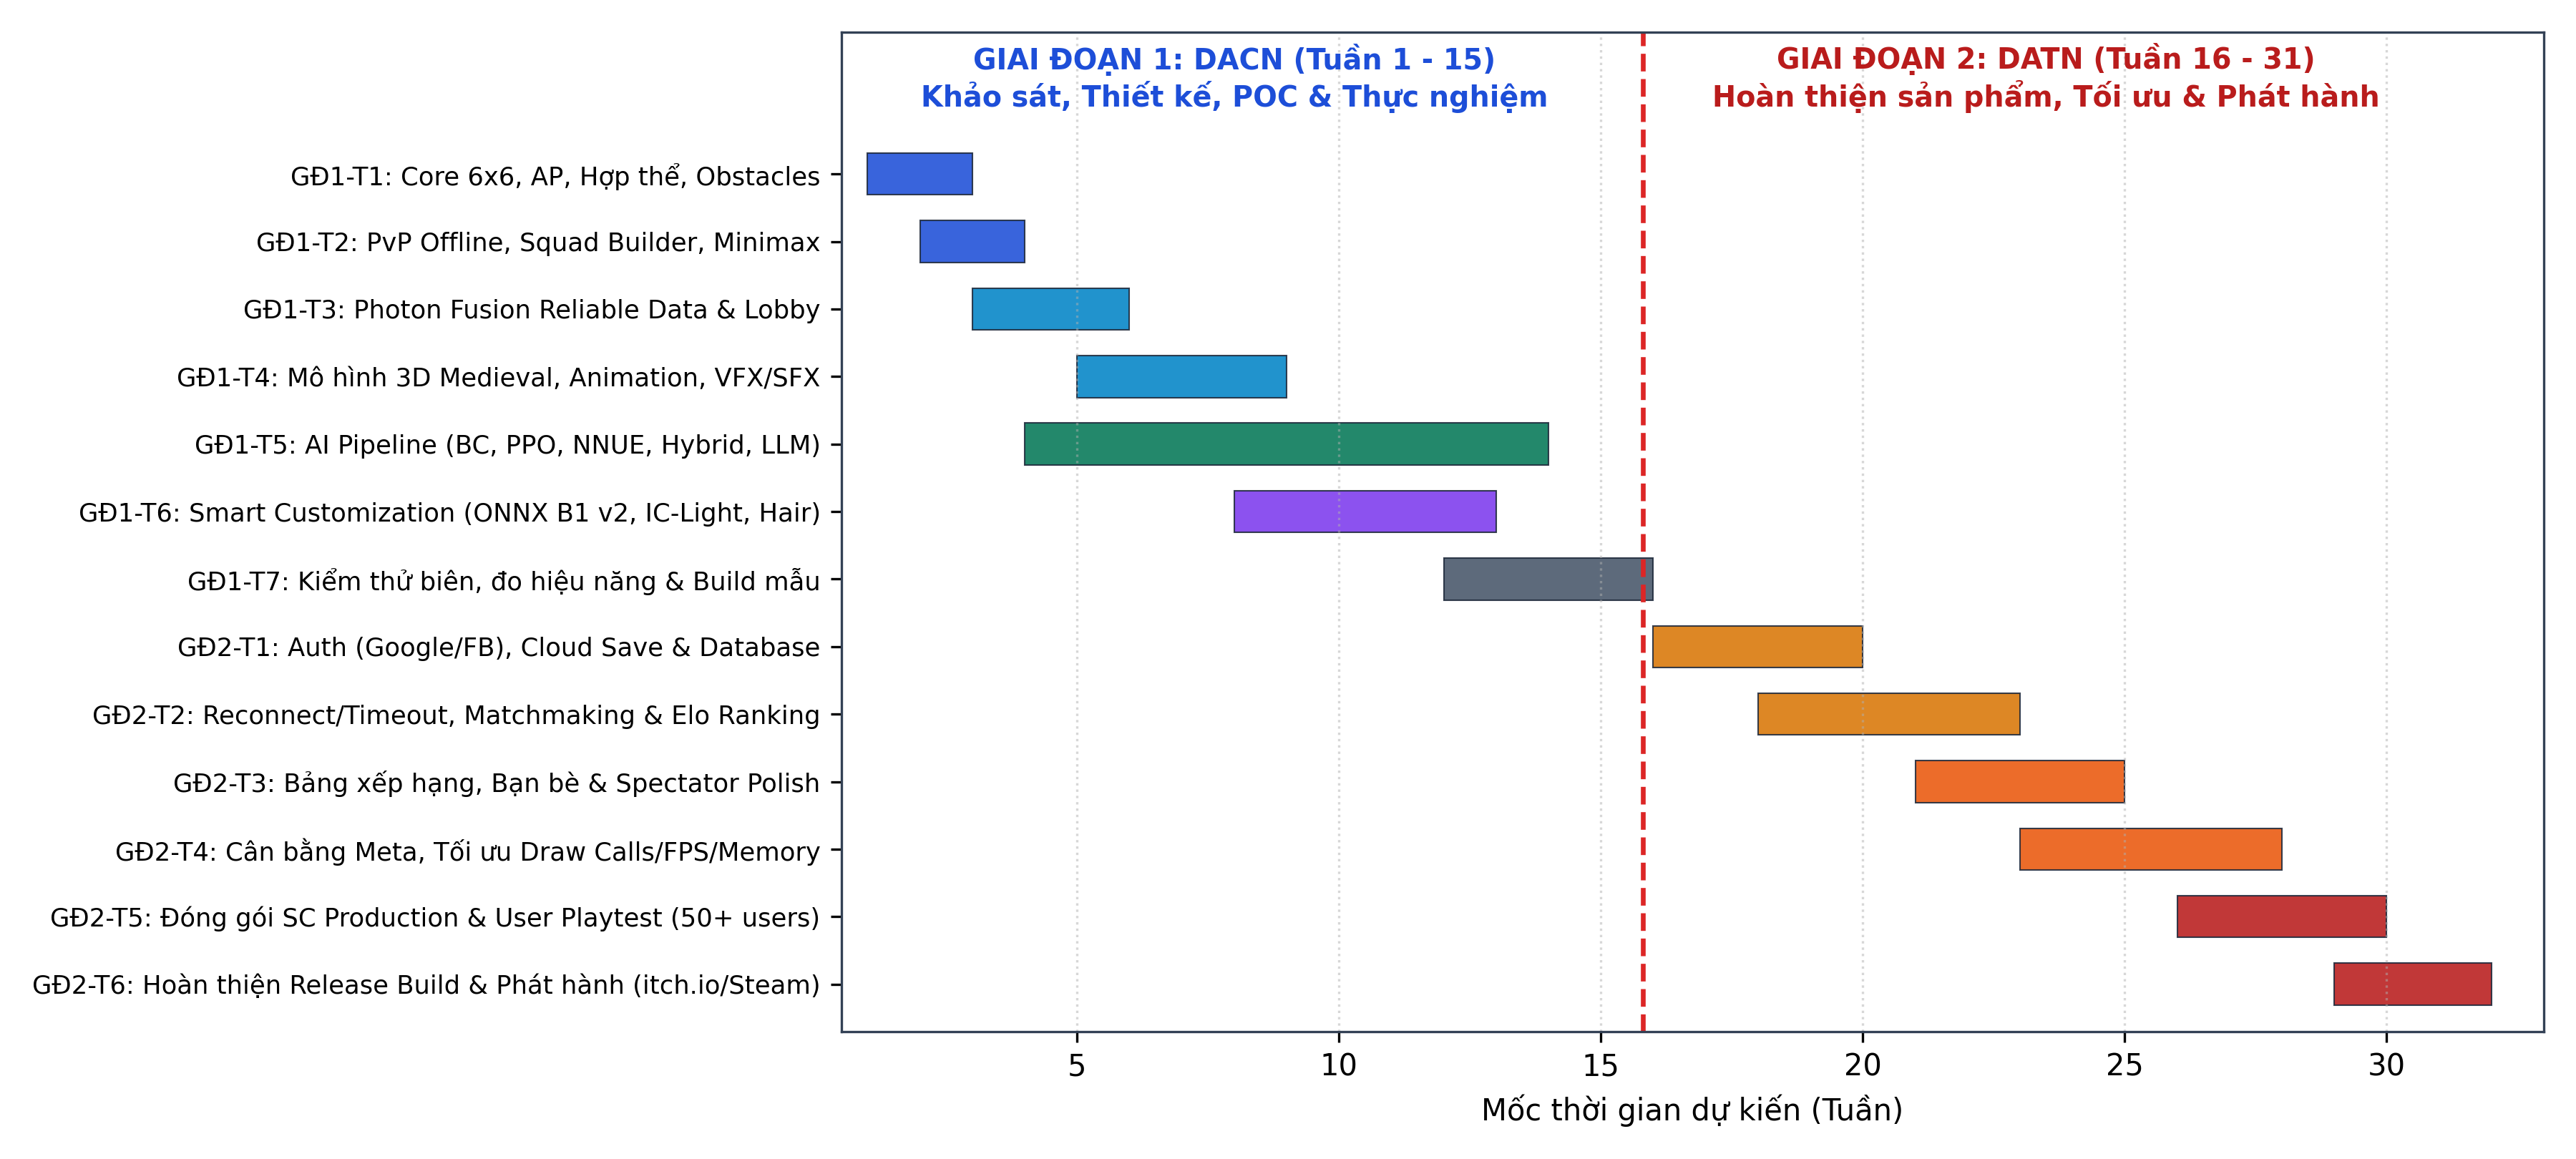
\includegraphics[width=\textwidth]{Diagrams/images/chart_roadmap_gantt.png}
    \caption{Lộ trình tổng thể hai giai đoạn từ Đồ án chuyên ngành (Tuần 1--15) sang Đồ án tốt nghiệp (Tuần 16--31)}
    \label{fig:roadmap_gantt}
\end{figure}

{\small
\begin{longtable}{L{2.5cm} L{2.0cm} L{5.7cm} L{4.7cm}}
    \caption{Kế hoạch chi tiết triển khai giai đoạn 2 (Đồ án tốt nghiệp -- DATN) hướng tới hoàn thiện và phát hành}
    \label{tab:stage2_plan} \\
    \toprule
    \textbf{Giai đoạn con} & \textbf{Mốc thời gian} & \textbf{Hạng mục công việc trọng tâm} & \textbf{Sản phẩm đầu ra (Deliverables)} \\
    \midrule
    \endfirsthead
    \toprule
    \textbf{Giai đoạn con} & \textbf{Mốc thời gian} & \textbf{Hạng mục công việc trọng tâm} & \textbf{Sản phẩm đầu ra (Deliverables)} \\
    \midrule
    \endhead
    \bottomrule
    \endfoot
        Pha 2.1: Hạ tầng tài khoản và dữ liệu đám mây & Tuần 16 -- 19 & Tích hợp đăng nhập Firebase Auth / Google / Facebook; thiết kế CSDL đám mây (Firestore / PlayFab) lưu hồ sơ người chơi, đội hình, lịch sử đấu và tham số avatar SC. & Hệ thống tài khoản đa thiết bị, Cloud Save thay thế lưu cục bộ đơn lẻ, lược đồ ERD hoàn chỉnh. \\
        \midrule
        Pha 2.2: Ổn định mạng, Matchmaking và Elo & Tuần 18 -- 22 & Hoàn thiện xử lý timeout, grace period và cơ chế Reconnect đồng bộ lại toàn bộ \texttt{GameState}; xây dựng hàng đợi ghép trận tự động (Matchmaking) và thuật toán tính điểm Elo; cân nhắc nâng cấp kiến trúc kiểm soát chống gian lận phía server (Authoritative Validation). & Chế độ Đấu hạng (Ranked PvP Online) ổn định trước sự cố ngắt mạng; vượt qua kiểm thử mô phỏng rớt gói $5\%$--$10\%$. \\
        \midrule
        Pha 2.3: Hệ thống xã hội và hoàn thiện luật chơi & Tuần 21 -- 24 & Xây dựng Bảng xếp hạng (Leaderboard), Danh sách bạn bè (mời đấu trực tiếp), xem lại đội hình người chơi; hoàn thiện luật hòa lặp thế cờ 3 lần (Zobrist History) và chế độ Khán giả nâng cao (Replay/Spectator HUD). & Màn hình Leaderboard, Friends System, Match History và bộ luật chuẩn giải đấu không còn tình huống biên mở. \\
        \midrule
        Pha 2.4: Cân bằng Meta AI, tối ưu hóa và hướng dẫn & Tuần 23 -- 27 & Phân tầng độ khó Bot PvE (Dễ: Heuristic D1/D2; Trung bình: PPO/NeuralMinimax; Khó: Residual NNUE / Hybrid / LLM); chạy mô phỏng $10{,}000+$ ván cân bằng tỷ lệ thắng đi trước/đi sau và chi phí AP/Slot; tối ưu Draw Calls (Static/GPU Batching, LOD, Object Pooling VFX), kiểm soát Memory/GC; xây dựng Interactive Tutorial. & Báo cáo profiling trước/sau tối ưu ($\ge 60$ FPS ổn định trên máy cấu hình thấp); bộ 4 cấp độ AI phục vụ người chơi; màn hướng dẫn tân thủ. \\
        \midrule
        Pha 2.5: Đóng gói SC, Playtest và phát hành & Tuần 26 -- 31 & Đóng gói dịch vụ Smart Customization (Docker GPU Cloud API hoặc chế độ Fallback nhẹ khi ngoại tuyến); tổ chức kiểm thử người dùng (Closed/Open Beta với $\ge 50$ người chơi) thu thập telemetry và bảng hỏi UX (SUS/GEQ); sửa lỗi cuối cùng và phát hành bản cài đặt Windows hoàn chỉnh. & Bản phát hành công khai trên itch.io / Steam Demo; tập dữ liệu khảo sát người dùng và báo cáo khóa luận tốt nghiệp hoàn chỉnh. \\
\end{longtable}
}

\newpage
\begin{thebibliography}{99}

\bibitem{unity6}
Unity Technologies, \textit{Unity 6 User Manual and Universal Render Pipeline (URP) Documentation}, 2025--2026. Truy cập tại: \url{https://docs.unity3d.com/}

\bibitem{photon_fusion}
Exit Games, \textit{Photon Fusion 2 Documentation -- Reliable Data Transfer, Shared/Host Topologies and NetworkRunner Callbacks}, 2025. Truy cập tại: \url{https://doc.photonengine.com/fusion/current/}

\bibitem{mlagents}
Juliani, A., Berges, V. P., Teng, E., Cohen, A., Harper, J., Elion, C., Goy, C., Gao, Y., Henry, H., Mattar, M., \& Lange, D., \textit{Unity: A General Platform for Intelligent Agents}, arXiv preprint arXiv:1809.02627, 2020. Truy cập tại: \url{https://github.com/Unity-Technologies/ml-agents}

\bibitem{ppo}
Schulman, J., Wolski, F., Dhariwal, P., Radford, A., \& Klimov, O., \textit{Proximal Policy Optimization Algorithms}, arXiv preprint arXiv:1707.06347, 2017.

\bibitem{potential_shaping}
Ng, A. Y., Harada, D., \& Russell, S., \textit{Policy invariance under reward transformations: Theory and application to reward shaping}, Proceedings of the Sixteenth International Conference on Machine Learning (ICML), pp. 278--287, 1999.

\bibitem{dagger}
Ross, S., Gordon, G., \& Bagnell, D., \textit{A Reduction of Imitation Learning and Structured Prediction to No-Regret Online Learning (DAgger)}, Proceedings of the Fourteenth International Conference on Artificial Intelligence and Statistics (AISTATS), pp. 627--635, 2011.

\bibitem{nnue}
Nasu, Y., \textit{Efficiently Updatable Neural-Network-based Evaluation Functions for Computer Shogi (NNUE)}, 28th World Computer Shogi Championship Appeal Document, 2018; và Stockfish Developers, \textit{Stockfish NNUE Architecture Documentation}, 2024.

\bibitem{funsearch}
Romera-Paredes, B., Barekatain, M., Novikov, A., Balog, M., Kumar, M. P., Dupont, E., Ruiz, F. J. R., Ellenberg, J. S., Wang, P., Fawzi, O., Kohli, P., \& Fawzi, A., \textit{Mathematical discoveries from program search with large language models (FunSearch)}, Nature, vol. 625, pp. 468--475, 2024.

\bibitem{cockburn}
Cockburn, A., \textit{Hexagonal Architecture (Ports and Adapters Pattern)}, 2005. Truy cập tại: \url{https://alistair.cockburn.us/hexagonal-architecture/}

\bibitem{mediapipe}
Lugaresi, C., Tang, J., Nash, H., McClanahan, C., Uboweja, E., Hays, M., Zhang, F., Chang, C. L., Yong, M. G., Lee, J., Chang, W. T., Hua, W., Georg, M., \& Grundmann, M., \textit{MediaPipe: A Framework for Building Perception Pipelines}, arXiv preprint arXiv:1906.08172, 2019.

\bibitem{mpfb2}
MakeHuman Community, \textit{MPFB2 -- MakeHuman Plugin For Blender Documentation and Python API}, 2025. Truy cập tại: \url{http://static.makehumancommunity.org/mpfb.html}

\bibitem{iclight}
Zhang, L., Rao, A., \& Agrawala, M., \textit{Scaling In-the-Wild Training for Diffusion-based Illumination Harmonization and Editing by Imposing Consistent Light Transport (IC-Light)}, ICLR, 2025.

\bibitem{hrn}
Lei, B., Ren, J., Feng, M., Cui, M., \& Xie, X., \textit{A Hierarchical Representation Network for Accurate and Detailed Face Reconstruction from In-The-Wild Images (HRN)}, Proceedings of the IEEE/CVF Conference on Computer Vision and Pattern Recognition (CVPR), pp. 394--403, 2023.

\bibitem{pytorch3d}
Ravi, N., Reizenstein, J., Novotny, D., Gordon, T., Lo, W. Y., Johnson, J., \& Gkioxari, G., \textit{Accelerating 3D Deep Learning with PyTorch3D}, arXiv preprint arXiv:2007.08501, 2020.

\end{thebibliography}


\end{document}
